% This is the root file of your thesis: thesis.tex
% A line starting with % is a comment. In some cases, I have included a command preceded by a %. You may activate the command by removing the %.

%%===================================
%%%%%%%%%%%%%%%%%%%%%%%%%%%%%%%%%%%%%%%%%%%%%%%%%%%%%%%%%%%%%%%%%%
%                           Document style
%%%%%%%%%%%%%%%%%%%%%%%%%%%%%%%%%%%%%%%%%%%%%%%%%%%%%%%%%%%%%%%%%%

\documentclass[12pt]{report}
\usepackage{ramsstyle}
%\documentclass{article}
\usepackage{graphicx}
\usepackage{caption}
%\DeclareCaptionJustification{justification=⟨RaggedRight⟩}

%%===================================
%Write the various parts of your thesis as separate files and include them into the main file by the command \include{name of included file}. When you compile the LaTeX file, you may choose which subfiles to include by the command

%\includeonly{chapter01,chapter02}

%%===================================
\begin{document}
%%%%%%%%%%%%%%%%%%%%%%%%%%%%%%%%%%%%%%%%%%%%%%%%%%%%%%%%%%%%%%%%%%%
%                   Command for the first page 
%%%%%%%%%%%%%%%%%%%%%%%%%%%%%%%%%%%%%%%%%%%%%%%%%%%%%%%%%%%%%%%%%%

\newcommand*\FirstPage{
\thispagestyle{empty}
% placing a pdf as background and adding text on top

\includepdf[pages=1,picturecommand*={ 
                % selecting placement, font size and text type
                \put(130,630){\fontsize{28}{28}\selectfont{\textsc{\textbf{Spicy Title}}}}
                \put(130,200){\fontsize{28}{28}\selectfont{\Large{\textbf{Teknisk rapportmal}}}}
                \put(130,180){\fontsize{28}{28}\selectfont{\Large{\textbf{NTNU studenter}}}}
                \put(130,160){\fontsize{28}{28}\selectfont{\Large{\textbf{Trondheim, vår 2020}}}}
                }]{images/ntnu_front_page.pdf}}

%This is the Titlepage
%%=========================================
\thispagestyle{empty}
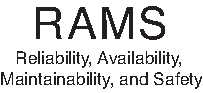
\includegraphics[scale=1.1]{fig/rams}
\mbox{}\\[6pc]
\begin{center}
\Huge{Resilience to Sea Level Extremes in Trondheim}\\[2pc]

\Large{Amy Anne McCormack}\\[1pc]
\large{Novermber 2022}\\[2pc]

PROJECT THESIS\\
Department of Geography\\
Norwegian University of Science and Technology
\end{center}
\vfill

\noindent Supervisor 1: Associate Professor Chantel Nixon

\noindent Supervisor 2: Associate Professor Martina Calovi

 % dont include will be generated during submission to inspera
\setcounter{page}{0}
\pagenumbering{roman}
%This is the last chapter 
%%=========================================

%Abstract (one page, c.350 words)
%Short summary of the thesis
%• what you investigated
% how you did it
%what you found out

\addcontentsline{toc}{section}{Abstract}
\section{Abstract}

Norway’s resilience to sea level extremes is and has been a dynamic process. To better protect coastal infrastructure and populations an understanding of how this resilience is changing is required. Improving the resilience of human settlements is required by both UN SDG's 11 and 13. Resilience is impacted by many factors which can be considered as falling within three key systems:  natural, technological and social systems. These systems interplay to alter the level of resilience and risk within places. Sea level extremes are extremely localised hazard in Norway and the understanding of this risk needs to be at a regional rather than national or global level. Changing climate, population distribution, geological setting change the resilience to sea level extremes that places in Norway have. 
The purpose of this project is to determine resilience to sea level extremes in 4 key places in Trondheim and assist the creation of a framework for quickly and cheaply determining a places resilience to changing sea level extremes. Investigating the link between local knowledge and academic models of sea level change in Trondheim is part of this process, including investigating which factors make individuals more aware of the risks of sea level extremes. This was done using a survey. *add sentance summarising results*




%This is the Acknowledgment
%%=========================================
\addcontentsline{toc}{section}{Acknowledgment}
\section*{Acknowledgment}
I would like to thank the following persons for their great help during this project. Chantel Nixon, Martina Cavoli. Callum Sinclair. NARM writing group. Everyone who brought me a cup of tea as I wrote this. \ldots



\begin{flushright}
A.A.M\\[1pc]

\end{flushright}
\tableofcontents
\listoffigures
\listoftables
\setcounter{page}{0}
\pagenumbering{arabic}
%This is chapter 1
%%=========================================
\chapter{Introduction}
The first chapter of a well-structured thesis is always an introduction, setting the scene with background, problem description, objectives, limitations, and then looking ahead to summarize what is in the rest of the report. This is the part that readers look at first---\emph{so make sure it hooks them!}


%-UN SDGS DEMAND MORE RESILIENCE
%-RESILEINCE IS DYNAMIC AND CHANGING
%REQUIRE FRAMEWORK TO QUICKLY & CHEAPLY DETERMINE RESILIENCE
%-SO WE CAN SEE HOW IT CHANGES
%- THIS IS AN ATTEMPT TO ASSIST THE CREATION OF SUCH A FRAMEWORK 
%- ASPECTS OF RESILIENCE - NATURAL, SOCIAL, TECHNOLOGICAL SYSTEMS

%%=========================================
\section{Background}
In this section, you should present the problem that you are going to investigate or analyze; why this problem is of interest; what has, so far, been done to solve the problem, and which parts of the problem that remain.
%%=========================================
\subsection*{Problem Formulation}
You should define your problem in a clear an unambiguous way and explain why this is a problem, why it is of interest---and to whom. It is also important to delimit the problem area.

\section{Project Purpose}
To determine the resilience to sea level extremes in 4 key places in Trondheim. To assist creation of framework for quickly and cheaply determining a places resilience to changing sea level extremes. to connect local knowledge to academic knowledge and assist in increasing awareness of the potential of sea level extremes in Trondheim. 

\section{Research Question}
\boldsymbol{R1} How resilient will Trondheim be to SLE’s during $2022-2050 and 2050 -2100$
\boldsymbol{R2}Are stakeholders aware about changes to SLE’s?
\boldsymbol{R3}What factors impact stakeholders’ awareness of SLEs ?

BREAKS DOWN INTO HYPOTHESIS
%%=========================================
\subsection*{Literature Survey}
You should here present the main books and articles that treat problems that are similar to what  you are studying. If you,  later in your thesis, describe the ``state of the art'' -- with a detailed literature survey, you may just give a very brief survey here (approx. a quarter of a page). If this is the only literature survey, you need to go into more details. An objective of the literature survey is to show the reader that you are familiar with the main literature within your field of research -- so that you do not ``reinvent the wheel.''


References to literature can be given in two different ways:
\begin{itemize}
\item As an \emph{explicit} reference: It is shown by \citet{lundteigen08} and partly also by \citet{rausand04}  that \ldots.
\item As an \emph{implicit} reference: It is shown \citep[e.g., see][Chap. 4]{rausand04} that \ldots.
\end{itemize}
In the example above, we have used ``author-year'' references, which is the preferred format. 
\begin{remark}
Following agreement with your supervisor, you may also refer by numbers, for example,  [1]. To do this, open the file \texttt{ramsstyle.sty} and  comment out (by \%) the command \texttt{$\backslash$usepackage\{natbib\}} and un-comment the corresponding command \texttt{$\backslash$usepackage[numbers]\{natbib\}}.\footnote{Notice the strange way we have to write the ``backslash'' in the text. This is because the ``backslash'' is a command in \LaTeX.}
\end{remark}
 You may include a link to the Internet in the text or in a footnote by using a command like: \url{http://www.ntnu.edu/ross}. 

When you refer to the scientific literature, you should always write in \emph{present} tense. Example: \citet{rausand04} show that \ldots.

\begin{remark}
Hyperlinks are included by the command \texttt{$\backslash$usepackage\{hyperref}\} in \texttt{ramsstyle.sty}. If you feel that the hyperlinks are disturbing when you enter the text, or want to avoid the hyperlinks in printed text, you may either comment out or edit this command in \texttt{ramsstyle.sty}.
\end{remark}
%%=========================================
\subsection*{What Remains to be Done?}
After you have defined and delimited your problem -- and presented the relevant results found in the literature within this field, you should sum up which parts of the problem that remain to be solved.
%%=========================================
\section{Objectives}
The main objectives of this Master's project are
\begin{enumerate}
\item This is the first objective
\item This is the second objective
\item This is the third objective
\item More objectives
\end{enumerate}

All objectives shall be stated such that we, after having read the thesis, can see whether or not you have met the objective. ``To become familiar with \ldots'' is therefore not a suitable objective.

%%=========================================
\section{Limitations}
In this section you describe the limitations of your study. These may be related to the study object (physical limitations, operational limitations), to the thoroughness of the analysis, and so on.
%%=========================================
\section{Approach}
Here you should describe the (scientific) approach that you will use to solve the problem and meet your objectives. You should specify the approach for each objective.

If there are any ethical problems related to your approach, these should be highlighted and discussed.
%%=========================================
\section{Structure of the Report}
The rest of the report is structured as follows. Chapter 2 gives an introduction to \ldots

\begin{remark}
Notice that chapter and section headings shall be written in lowercase, but that all main words should start with a capital letter.
\end{remark}


The report should be no longer than \underline{60 pages} in this format 
%%This is chapter 2
%%=========================================
\chapter[Equations, etc]{Equations, Figures, and Tables}
The content of this chapter will vary with the topic of your thesis. 
\begin{remark}
If you want a shorter chapter or section title to appear in the Table of Contents and in the headings of the chapter, you just include the short title in square brackets before the title of the chapter/section.
\end{remark}

%%=========================================
\section{Simple Equations}
This is how a simple equation is included:
\begin{equation}
F(t)=\int_0^t \exp(-\lambda x)\,dx
\label{eq1}
\end{equation}

The equations are automatically given equation numbers -- here (\ref{eq1}) since this is the first equation in Chapter 2. Note that you can refer to the equation by referring to the ``label'' you specified as part of the equation environment.

You can also include equations without numbers:
\begin{equation*}
F(t)=\sum_{i=1}^n \binom{n}{i}\sin(i\cdot t)
\end{equation*}

%%=========================================
\subsection*{More Advanced Formulas}
Please consult the \LaTeX\ documentation.

If you want to include a definition of a term/concept in the text, I have made the following macro (see in \texttt{ramsstyle.sty}):
\begin{defin}
\textbf{Reliability}: The ability of an item to perform a required function under stated environmental and operational conditions and for a stated period of time.
\end{defin}

%%=========================================
\section{Including Figures}
If you use pdf\LaTeX\ (as recommended), all the figures must be in pdf, png, or jpg format. We recommend you to use the pdf format.  Please place the figure files in the directory \textbf{fig}. Figures are included by the command shown for Figure~\ref{fig1}. Please notice the ``path'' to the figure file written by a \emph{forward} slash (/). You should not include the format of the figure file (pdg, png, or jpg) -- just write the ``name'' of the figure. 
\begin{figure}
\centering

\includegraphics[scale=0.6,angle=15]{fig/NTNU}
\caption{This is the logo of NTNU (rotated 15 degrees).}
\label{fig1}
\end{figure}

Each figure should include a unique \emph{label} as shown in the command for Figure~\ref{fig1}. You can then refer to the figure by the \emph{ref} command.
Notice that you can scale the size of the figure by the option \texttt{scale=k}. You may also define a specific width or height of the figure by replacing the \texttt{scale} options by \texttt{width=k} or \texttt{height=k}. The factor \texttt{k} can here be specified in mm, cm, pc, and many other length measures. You may also give \texttt{k} as a fraction of the width of the text or of the height of the text, for example, \texttt{width=0.45$\backslash$textwidth}. If you later change the margins of the text, the figure width will change accordingly. As illustrated in Figure~\ref{fig1}, you may also rotate the figure -- and also do many other things (please check the documentation of the package \texttt{graphicx} -- it is available on your computer, or you may find it on the Internet).

In \LaTeX\ all figures are floating objects and will normally be placed at the top of a page. This is the standard option in all scientific reports. If you insist on placing the figure exactly where you declare the figure, you may include the command \texttt{[h]} (here) immediately after $\backslash$\texttt{begin\{figure\}}. If you will force the figure to be located either at the top or bottom of the page, you may alternatively use  \texttt{[t]} or \texttt{[b]}. For more options, check the documentation.

Large figures may be included as a \emph{sidewaysfigure} as shown in Figure~\ref{fig2}:\footnote{You can use a similar command for large tables.}
\begin{sidewaysfigure}
\centering

\includegraphics[scale=1.8]{fig/NTNU}
\caption{This is the logo of NTNU.}
\label{fig2}
\end{sidewaysfigure}

%%=========================================
\section{Including Tables}
\LaTeX\ has a lot of different options to include tables. Only one of them is illustrated here.

\begin{table}
	\centering\small
	\caption{The degree of newness of technology.}
	\label{tab1}
		\begin{tabular*}{\textwidth}{@{\extracolsep{\fill}}lccc}
			\toprule
			  &\multicolumn{3}{c}{Level of technology maturity}\\
  \cmidrule{2-4}
			Experience with the		   &  & Limited field history or not & New or \\
              operating  condition  & Proven &  used by company/user & unproven \\
        
			\midrule
			  Previous experience & 1 & 2 & 3 \\
		          No experience by company/user & 2 & 3 & 4 \\
		          No industry experience & 3 & 4 & 4 \\
			\bottomrule
		\end{tabular*}
\end{table}

\begin{remark}
Notice that figure captions (Figure text) shall be located \emph{below} the figure -- and that the caption of tables shall be \emph{above} the table. This is done by placing the $\backslash$\texttt{caption} command beneath the command $\backslash$\texttt{includegraphics} for figures, and above the command $\backslash$\texttt{begin\{tabular*\}} for tables.
\end{remark}
%%=========================================
\section{Copying Figures and Tables}
In some cases, it may be relevant to include figures and tables from from other publications in your report. This can be a direct copy or that you retype the table or redraw the figure. In both cases, you should include a reference to the source in the figure or table caption. The caption might then be written as: \textsl{Figure/Table xx: The caption text is coming here \citep{rausand04}.}

In other cases, you get the idea from a figure or table in a publication, but modify the figure/table to fit your purpose. If the change is significant, your caption should have the following format: \textsl{Figure/Table xx: The caption text is coming here \citep[adapted from][]{rausand04}.}

%%=========================================
\section{References to Figures and Tables}
Remember that all figures and tables shall be referred to and explained/discussed in the text. If a figure/table is not referred to in the text, it shall be deleted from the report.
%%=========================================
\section{A Word About Font-encoding}
When you press a button (or a combination of buttons) on your keyboard, this is represented in your computer according to the \emph{font-encoding} that has been set up. A wide range of font-encodings are available and it may be difficult to choose the ``best'' one. In the template, I have set up a font-encoding called UTF-8 which is a modern and very comprehensive encoding and is expected to be the standard encoding in the future. Before you start using this template, you should open the Preferences ->Editor dialogue in TeXworks (or TeXShop if you use a Mac) and check that encoding UTF-8 has been specified. 

If you use only numbers and letters used in standard English text, it is not very important which encoding you are using, but if you write the Norwegian letters æ, ø, å and accented letters, such as é and ä, you may run into problems if you use different encodings. Please be careful if you cut and paste text from other word-processors or editors into your \LaTeX\ file!

\subsubsection*{Warning}
If you (accidentally) open your file in another editor and this editor is set up with another font-encoding, your non-standard letters will likely come out wrong. If you do this, and detect the error, be sure \emph{not} to save your file in this editor!!

This is not a specific \LaTeX\ problem. You will run into the same problem with all editors and word-processors -- and it is of special importance if you use computers with different platforms (Windows, OSX, Linux).

%%=========================================
\section{Plagiarism}
Plagiarism is defined as ``use, without giving reasonable and appropriate credit to or acknowledging the author or source, of another person's original work, whether such work is made up of code, formulas, ideas, language, research, strategies, writing or other form'', and is a very serious issue in all academic work. You should adhere to the following rules:
\begin{itemize}
\item Give proper references to all the sources you are using as a basis for your work. The references should be give to the original work and not to newer sources that mention the original sources.
\item You may copy paragraphs up to 50 words when you include a proper reference. In doing so, you should place the copied text in inverted commas (i.e., ``Copied text follows \ldots''). Another option is to write the copied text as a quotation, for example:
\begin{quote}
Birnbaum's measure of reliability importance of component $i$ at time $t$ is equal to the probability that the system is in such a state at time $t$ that component $i$ is critical for the system.\newline \mbox{} \hfill \citet{rausand04}
\end{quote}
\end{itemize}




%automated figure captioning
\chapter{Background}

\section{Norway and SLEs in the Present Day}
 It would be reasonable to consider Norway's culture and socioeconomic position as dominated by its relationship with the sea. All of its major cities are located on the coast.  By January 2022, 31.6\% of Norway's coastal zone has been influenced by buildings, railways, roads and agriculture (\cite{engebakken_construction_2022}). This is notable as only 68.4\% of the Norwegian coastline is currently deemed accessible due to its steep terrain (\cite{engebakken_construction_2022}). Norwegian weather is predicted to become more extreme (\cite{rod_integrated_2012}), in line with global trends, which project increasing coastal flooding due to extreme weather and sea-level rise (\cite{hoffken_effects_2020}). 
\paragraph{}

Due to settlement patterns in Norway and the changing climate, the threat of natural hazards related to the sea is increasing, which requires increased attention to be given to regional vulnerability and the resilience of places (\cite{opach_seeking_2020}; \cite{rod_three_2015}). Quantitative community resilience measurement approaches have been tried, but there are several limiting factors including that they rarely offer policy makers the strategies required for building resilience (\cite{opach_seeking_2020}; \cite{gerkensmeier_governing_2018}). Important information can be gained from vulnerability indices, including better understanding of social vulnerability, but questions remain about how social vulnerability can be decreased to build resilience. 


\section{Introduction to Research Area}

Trondheim is situated deep within Trondheimsfjord, which protects it from the North Sea (figure \ref{fig:research_area}). The maximum observed sea level extreme in Trondheim is 2.60m (referring to elevation reference model NN2000), recorded in 1971 (\cite{kartverket_high_2022}). Trondheim municipality plans indicate that the city should be prepared for SLEs of 4.87m by 2100 (\cite{miljoenheten_og_byplankontoret_trondheim_kommune_9-notat-om-havnivastigning-og-stormflo---hensyn-i-arealplanlegging-nyhavnapdf_2020}. 
\paragraph{}
Trondheim can be considered one of the most resilient places in Norway due to its protected location, geological setting, infrastructure and socioeconomic status (\cite{opach_seeking_2020}). Thus, it would be reasonable to assume that unlike other places in Norway the infrastructure in Trondheim is not at risk from SLEs (\cite{baisotti_farevarsel_2020}). Such an assumption can be backed up by the knowledge of the fact that the Earth's crust below Norway is still rebounding due to deglaciation following the last ice age; a process known as glacioisostatic adjustment (\cite{breili_high-accuracy_2020}). What is perhaps less widely understood, is that glacioisostatic adjustment is an incredibly varied process across the country and the basic model that the majority of the population has about sea level-rise and land uplift, may be creating a false confidence, especially as weather events due to their uncertainty are often excluded from sea level rise projections  (\cite{breili_high-accuracy_2020}, \cite{hanssen-bauer_climate_2017}).  Furthermore the tidal patterns in Trondheimsfjord (\ref{fig:research_area}) are complex, as is often the case in deep fjords, adding another layer of uncertainty to the projections of changing sea levels (\cite{hanssen-bauer_climate_2017}).

\begin{figure}[H]
    \centering
    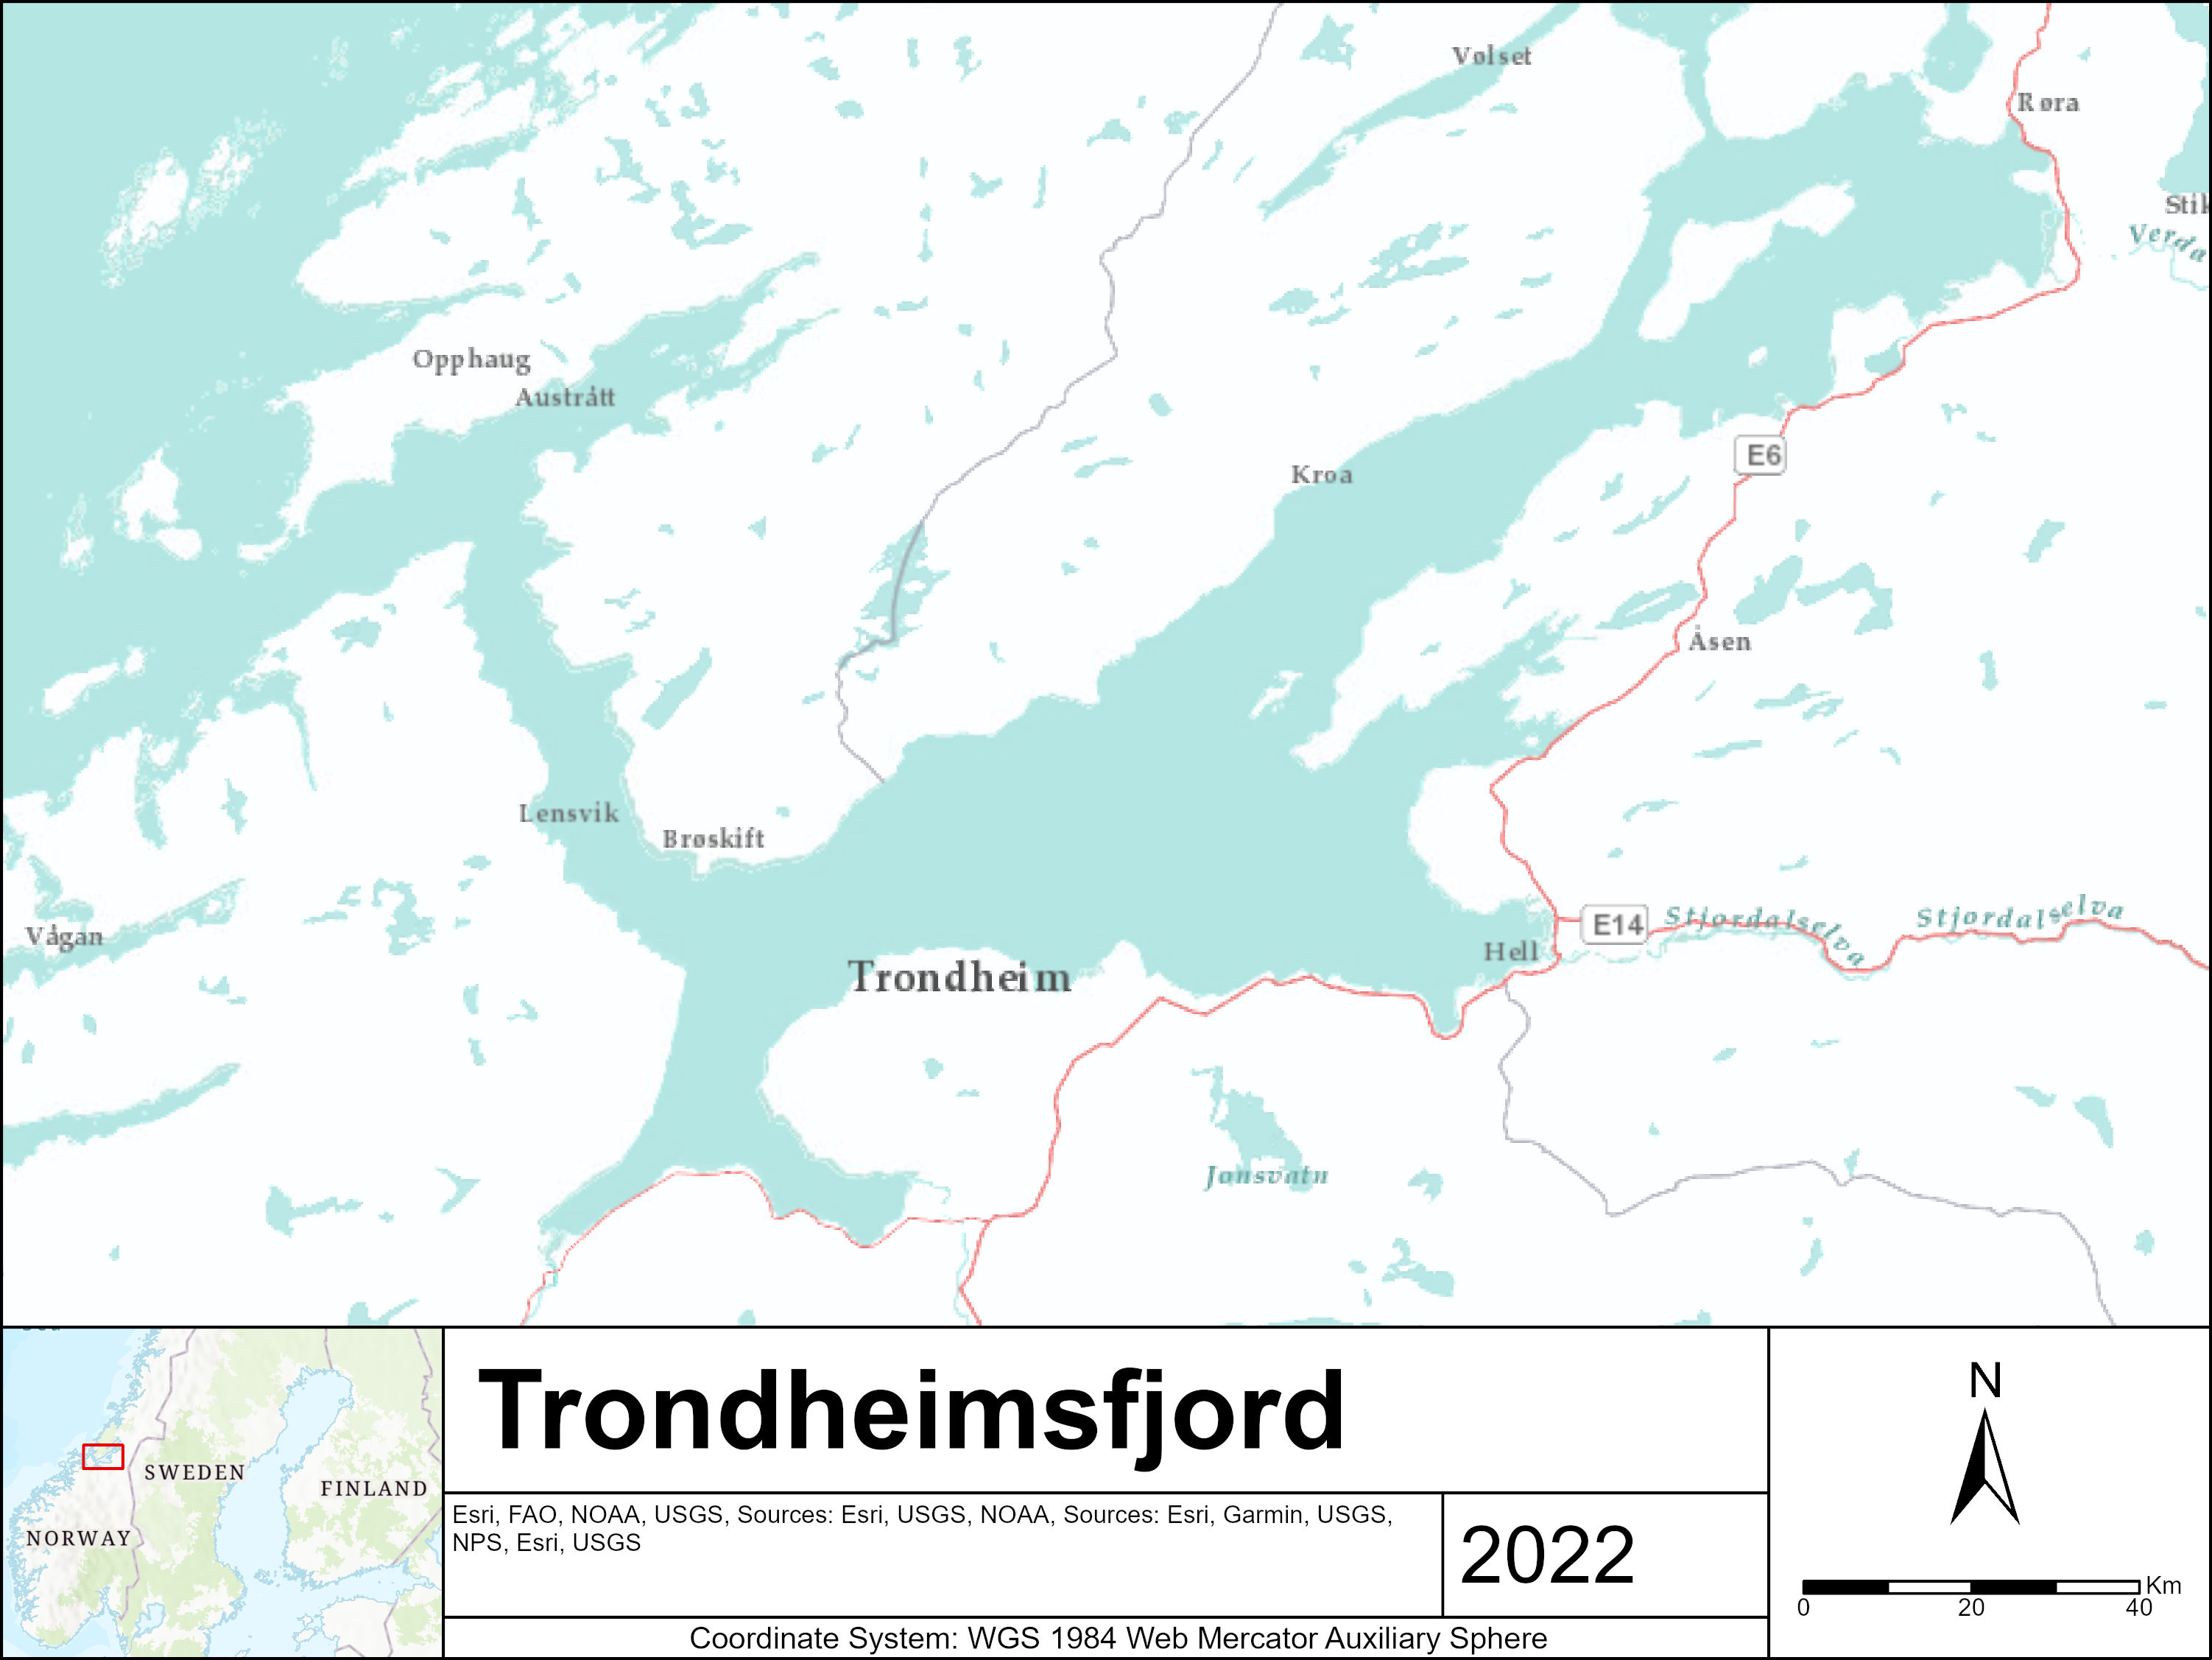
\includegraphics[width=1.0\textwidth]{fig/Trondheimsfjord.png}
    \caption[Research area - Trondheimsfjord]
    {The city of Trondheim is situated in Trondheimsfjord, which provides protection from the North Sea. The red line represents Norway's major road network. The E6, perhaps the most critical road infrastructure for Trondheim is shown as close to the coast. Figure created using ArcGIS Pro. }
    \label{fig:research_area}
    
\end{figure}



\section{Study Sites} \label{study-sites-background}
Four study sites situated on Trondheim's coast were chosen for their high daily population throughput, large amounts of infrastructure, and coastal characteristics. These are Brattøra, Grillstad, Skansen and Nidelva. Physical vulnerability to SLEs is diverse for these sites, as can be seen in figure ~\ref{fig:research_site} below and is further outlined in table ~\ref{table:research_site}. 
\paragraph{}

\begin{figure} [H]
    \centering
    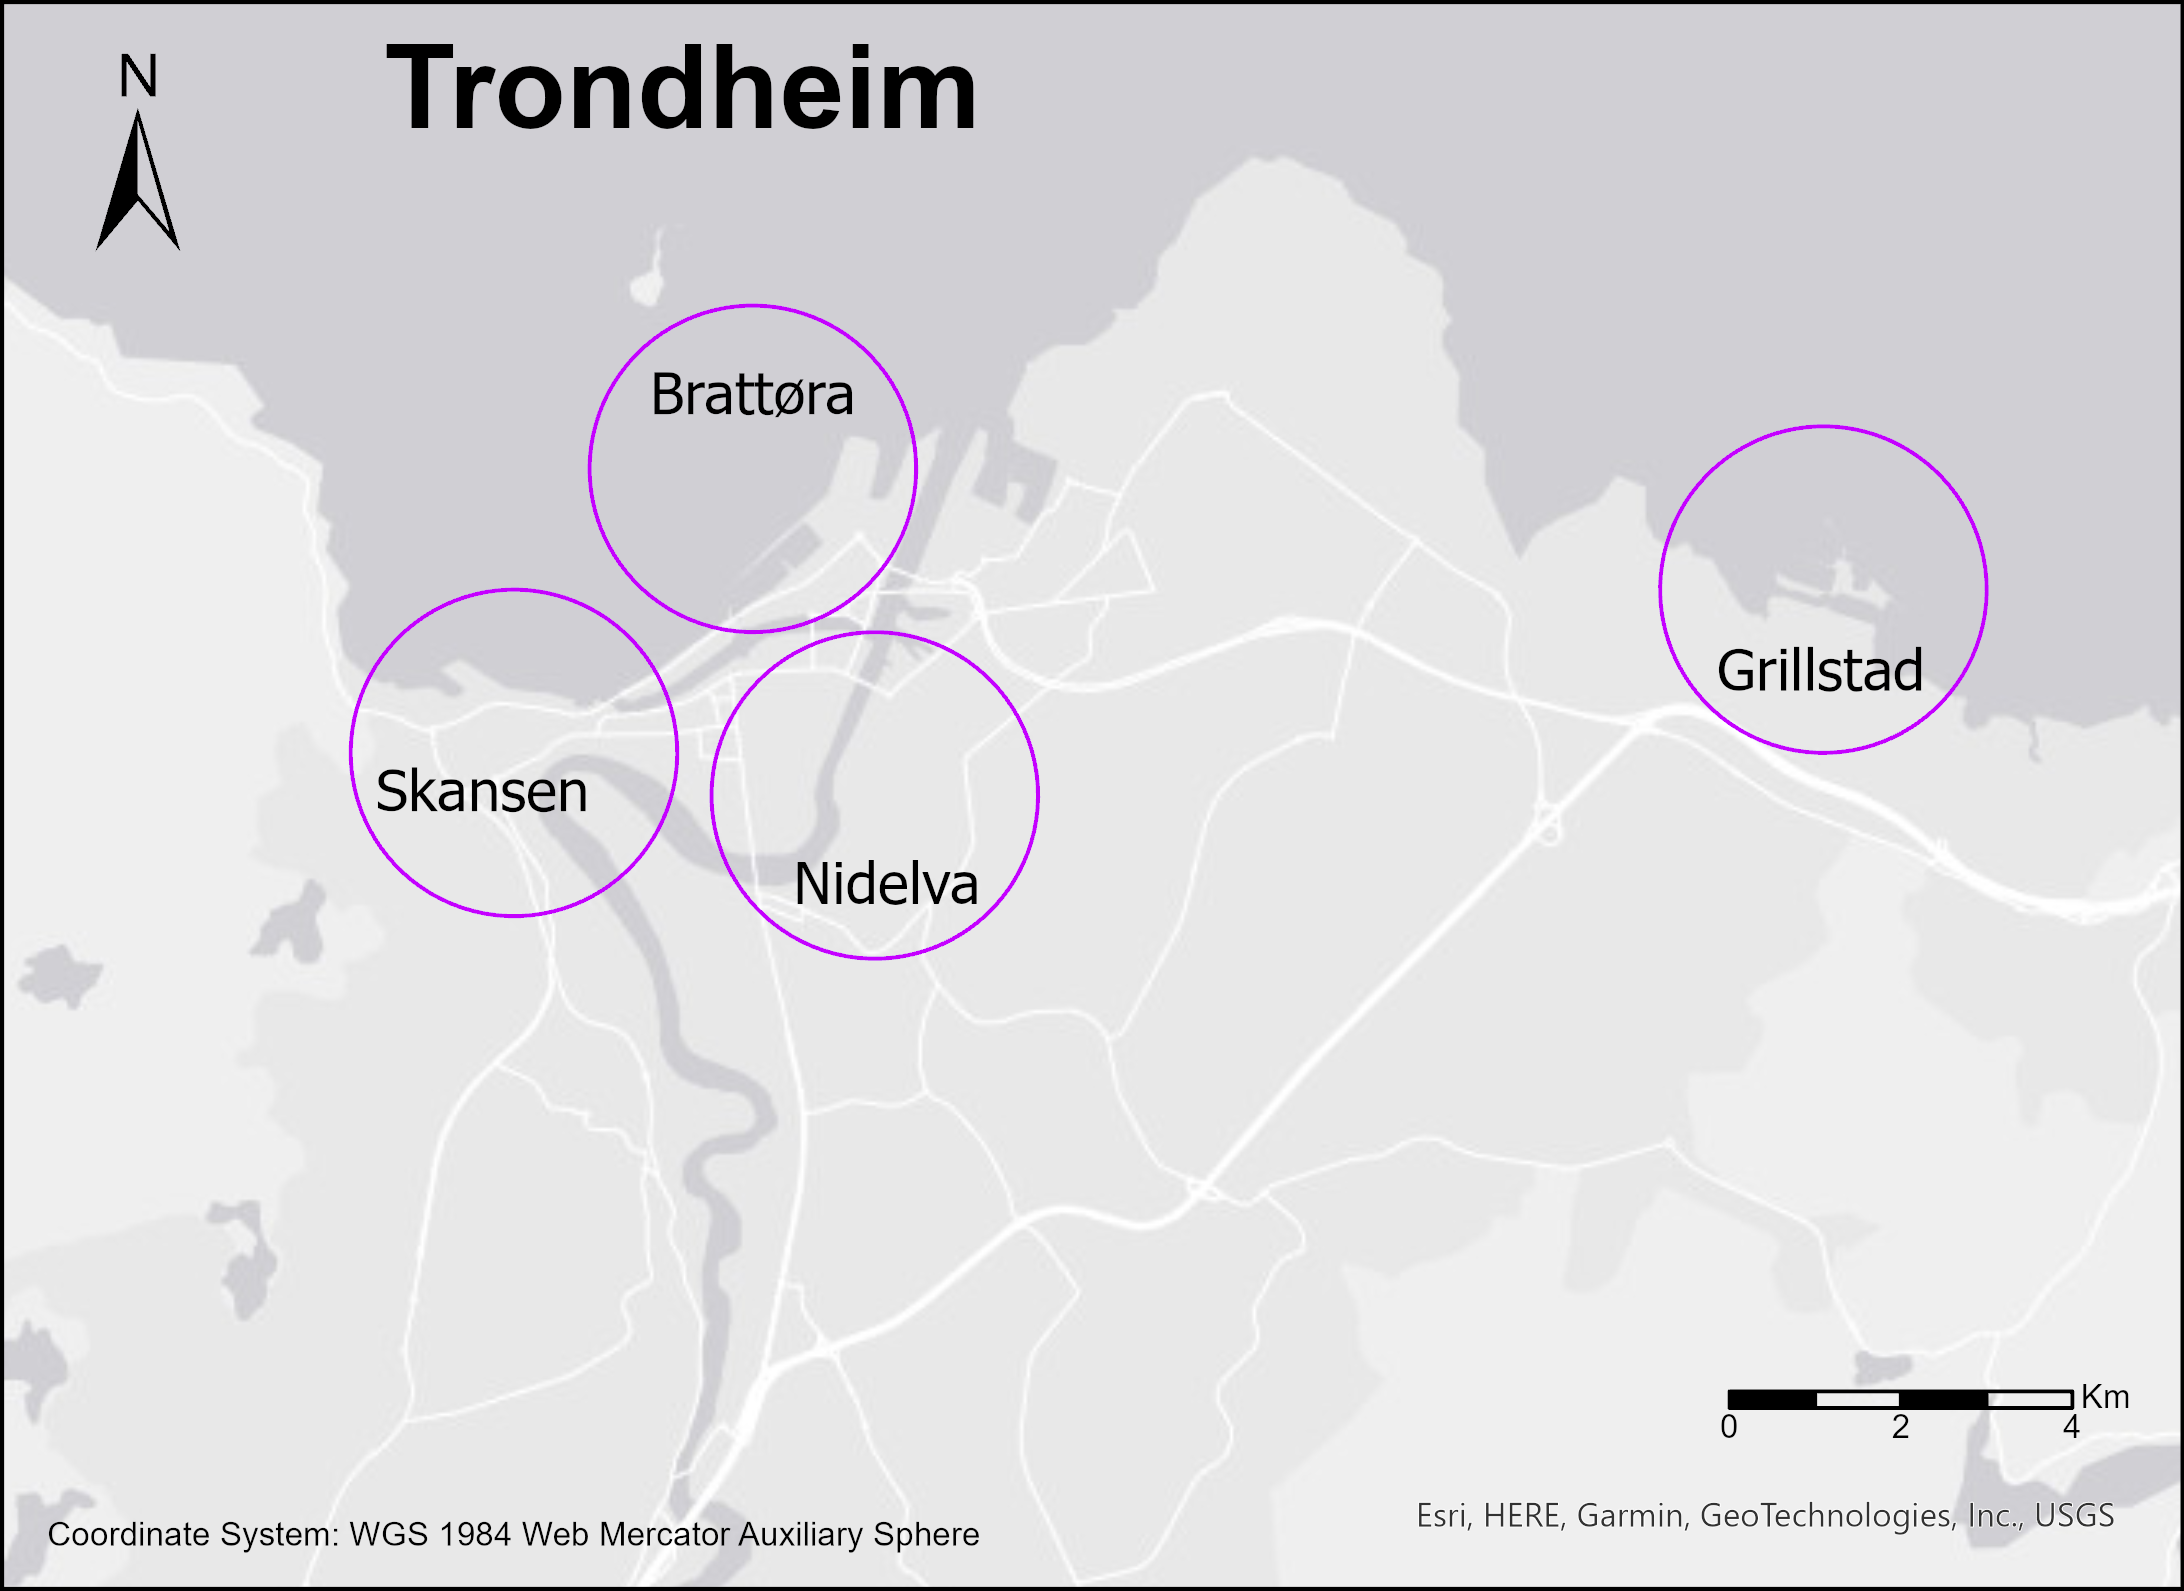
\includegraphics[width=1.0\textwidth]{fig/trondheim_research_sites_grey_circles.png}
    \caption[Research sites - Trondheim]{The sites chosen to investigate Trondheim are Brattøra, Grillstad, Skansen and Nidelva. These sites are highlighted with a purple circle. As shown here Brattøra has both the sea, canal and a section of artificially straightened tidal river within its site. Grillstad includes reclaimed land and an artificial island connected via a bridge. Nidelva takes its name from the river running through it. Nidelva research site is further from the open fjord , but includes marinas. Skansen has the sea and canal within its site, while its river is not straightened it is prevented from shifting. Figure was created using ArcGIS Pro.}
    \label{fig:research_site}
\end{figure}

\paragraph{}


Factors considered in defining physical vulnerability to sea-level rise (including SLEs) are: natural resistance to erosion, engineered resistance to erosion, engineered protection to SLEs, infrastructure built directly upon coastline, settlement patterns, usage patterns and projected changes in SLEs. The physical vulnerability was determined from direct observation,  models from \cite{kartverket_se_2021} and consulting planning documents for each site (\cite{miljoenheten_og_byplankontoret_trondheim_kommune_9-notat-om-havnivastigning-og-stormflo---hensyn-i-arealplanlegging-nyhavnapdf_2020}). 


\paragraph{}
\begin{table}[!ht]
    \centering
    \begin{tabular}{|l|l|l|l|l|}
    \hline
        \textbf{location} & \textbf{Brattøra} & \textbf{Grillstad} & \textbf{Skansen}  & \textbf{Nidelva} \\ \hline
       1950s' PV  & high & high & medium & low \\ \hline
       2022 PV  &  medium &  medium &  low &  low \\ \hline
       2090s' PV &  high &  high &  medium &  medium \\ \hline
        Dominant & office space  & residential & recreational  & residential and \\ \newline
        Use & and harbour &  only   &  and industry & and commercial  \\ \hline
        Land Type & reclaimed land & reclaimed land & managed coastline  & altered tidal river \\ \hline
        Protection & harbour wall & harbour wall & harbour wall, placed rocks & inland \\ \hline
    \end{tabular}
    \caption{ Research Sites Changing Physical Vulnerability to SLEs}{PV - Physical Vulnerability. Created from observation of the sites conducted in 2021 and \cite{kartverket_se_2021}}
    \label{table:research_site}
\end{table}

Brattøra is the research site with the least amount of residential population. Most buildings are occupied by offices and are protected by a harbour wall and a small harbour behind that (figure \ref{fig:research_site}). Brattøra is located on reclaimed land and for this reason it had a very high physical vulnerability to sea-level rise and SLEs 70 years ago. The modern harbour and area's design have lowered the physical vulnerability to medium now, but it is projected to have several areas that are flooded regularly by the 2090s (\cite{kartverket_se_2021}). Currently, the vulnerable areas in Brattøra are predominantly sustainable urban development schemes with footpaths and car parks located where the majority of current potential flooding would occur. However, there is still risk of more significant impacts from SLEs beyond nuisance flooding, such as erosion, disconnecting important transport routes (figure \ref{fig:research_site}) and preventing access to offices.
\paragraph{}
Grillstad is also located on reclaimed land, and like Brattøra, had a very high physical vulnerability in the 1950s. It is also located behind a harbour, including a harbour wall now, but in contrast to  Brattøra, the dominant land use is residential (Table \ref{table:research_site}). There are several small commercial ventures, but the vast majority serve the needs only of local residents. There are no major transport connections or industry at this site. 
\paragraph{}
Nidelva is a less obvious choice for research into SLEs as it is situated further from the coastline. The land type here is altered tidal river and its physical vulnerability 70 years ago was low. The dominant uses are residential and commercial and it has lower physical vulnerability predicted in 70 years than Brattøra and Grillstad (table \ref{table:research_site}). The Nidelva research site has the added complication of the river level potentially impacting the height of the water at certain times. The river here is controlled by the dam in Leirfoss, which is part of the hydroelectric power scheme which provides energy to the area (\cite{statkraft_leirfossene_2022}).
\paragraph{}
Skansen has two dominant uses of recreation and industry, however, there is also significant residency in the area, the majority being high-rise apartment buildings at least 10m from the coastline. While several aspects of this coastline may appear more natural, it is a managed coastline which is protected by placed rocks, a harbour wall and small bays. Unlike the other sites, there have been attempts to utilise natural techniques to prevent flooding in this area. This includes the restoration of Illabekken river and banks and the use of so-called living shorelines, in this case non-concreted areas which are covered in plants to improve infiltration (\cite{selliseth_ilabekken_2021}.
\paragraph{}

Brattøra, Skansen and Nidelva have previously been highlighted during case presentations by the municipality as areas that currently have a risk of temporary flooding (\cite{hanssen_saksframlegg_2013}). This risk level is projected to change over the next 100 years (\cite{hanssen-bauer_climate_2017}). This is why these areas have special building requirements such as water-tight basements and keeping electrical installations above the area of potential flooding (\cite{hanssen_saksframlegg_2013}). Grillstad was not specified in the report as it was built after publication, but it is located in the area requiring special building requirements so it can also be considered a vulnerable area. 







\section{ Natural System Resilience}

The datasets \cite{kartverket_se_2021} and \cite{ipcc_sea_2021} were used to create visual simulations and maps of SLEs for the research sites, further details in methodology section \ref{data-collection}. Section \ref{visual-simulations} and \ref{maps-sles} display these images to show Trondheim's vulnerable locations natural system resilience. 

\subsection{Visual Simulation of SLEs} \label{visual-simulations}
 Figures ~\ref{fig:SLE-nidelva} to ~\ref{fig:sle-skansen} display the simulated SLEs created for this project. 

\begin{figure}[H]
    \centering
    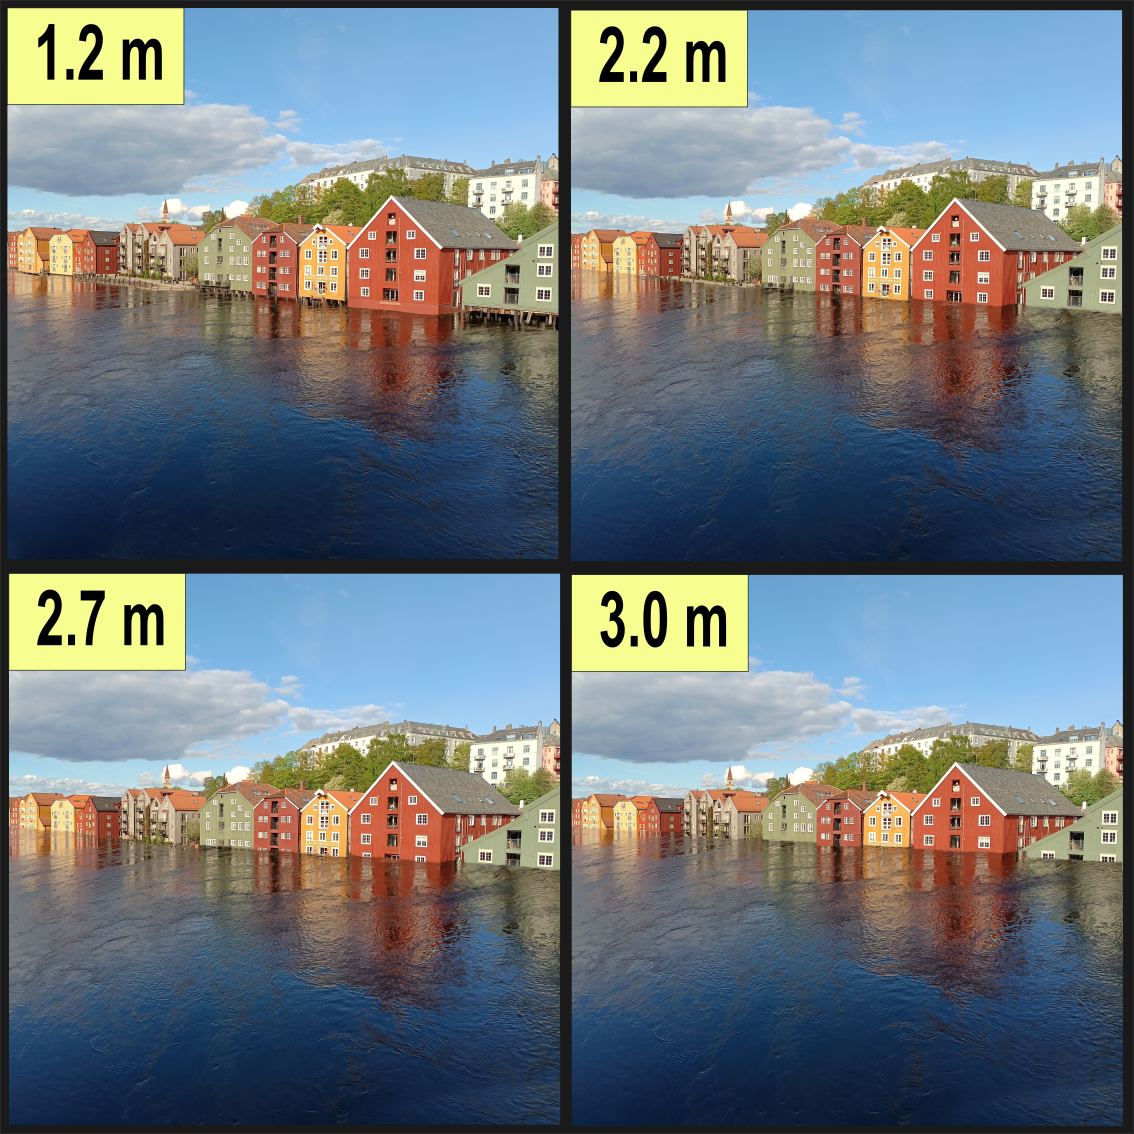
\includegraphics[width=16cm]{fig_sle/nidelva 2090 q.png}
    \caption{Simulated SLEs for Nidelva}
    {These were created using \cite{kartverket_se_2021}, Inkscape and GIMP.}
    \label{fig:SLE-nidelva}
\end{figure}

\begin{figure}[H]
    \centering
    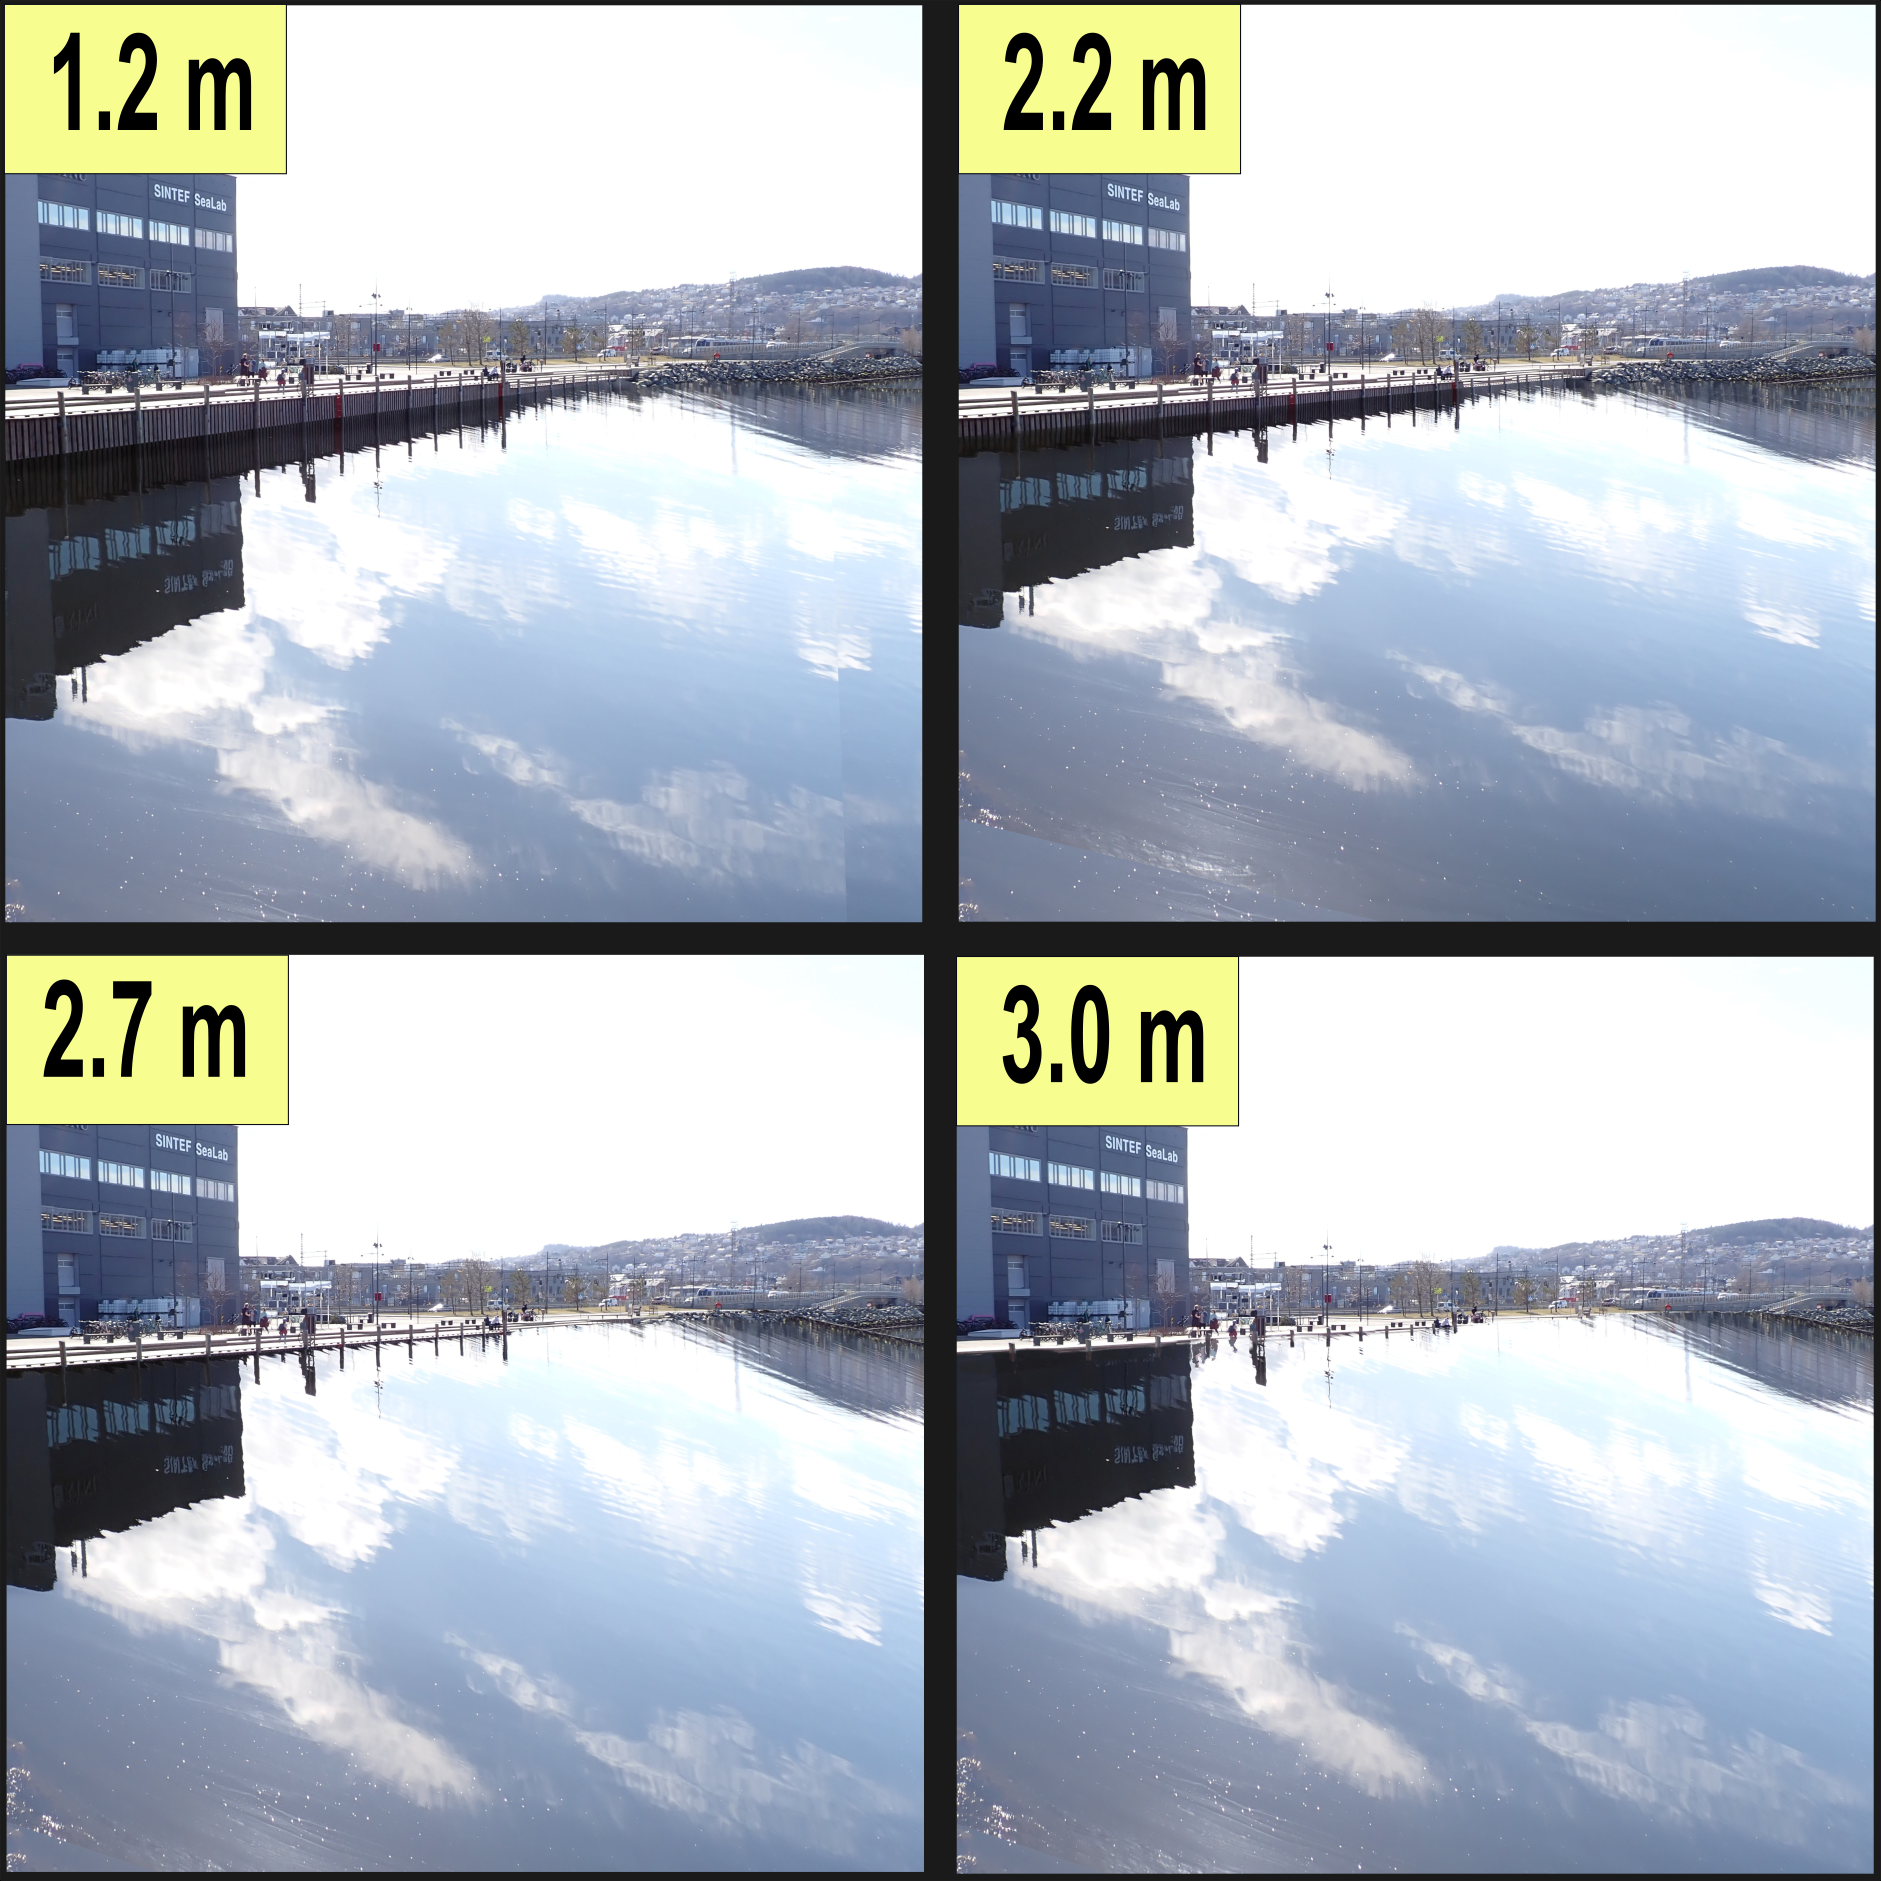
\includegraphics[width=16cm]{fig_sle/boxes top left - brattora sle.png}
    \caption{Simulated SLEs for Brattøra}
    {These were created using \cite{kartverket_se_2021}, Inkscape and GIMP. }
    \label{fig:SLE-brattora}
\end{figure}

\begin{figure}[H]
    \centering
    \includegraphics[width=16cm]{fig_sle/grillstad 2090 q.png}
    \caption{Simulated SLEs for Grillstad}{These were created using \cite{kartverket_se_2021}, Inkscape and GIMP. }
    \label{fig:SLE-grillstad}
\end{figure}

\begin{figure}[H]
    \centering
    \includegraphics[width=16cm]{fig_sle/illsvika 2090 q.png}
    \caption{Simulated SLEs for Skansen}{These were created using \cite{kartverket_se_2021}, Inkscape and GIMP. }
    \label{fig:sle-skansen}
\end{figure}


The differing heights represent different potential events. The top left square, 1.2m is a very likely event as this is the height associated with the spring high tide for each of the research sites. The top right square, 2.2m is a significantly less likely as it represents the water level height associated with the current 20 year storm surge, while a water level of 2.7m is projected for the 20 year storm surge in 2090. Finally, the 1000 year storm surge in 2090 is represented by 3.0m as seen in the bottom right square of each of the figures. The figures also display how natural systems interplay with technological systems.

\subsection{Maps of SLEs} \label{maps-sles}
Figures ~\ref{fig:sle_skansen_num} to ~\ref{fig:sle_nidelva_num}  display the mapped SLEs created for this thesis based off \cite{kartverket_se_2021} for the research sites - Skansen, Brattøra, Grillstad and Nidelva.

\begin{figure}[H]
    \centering
    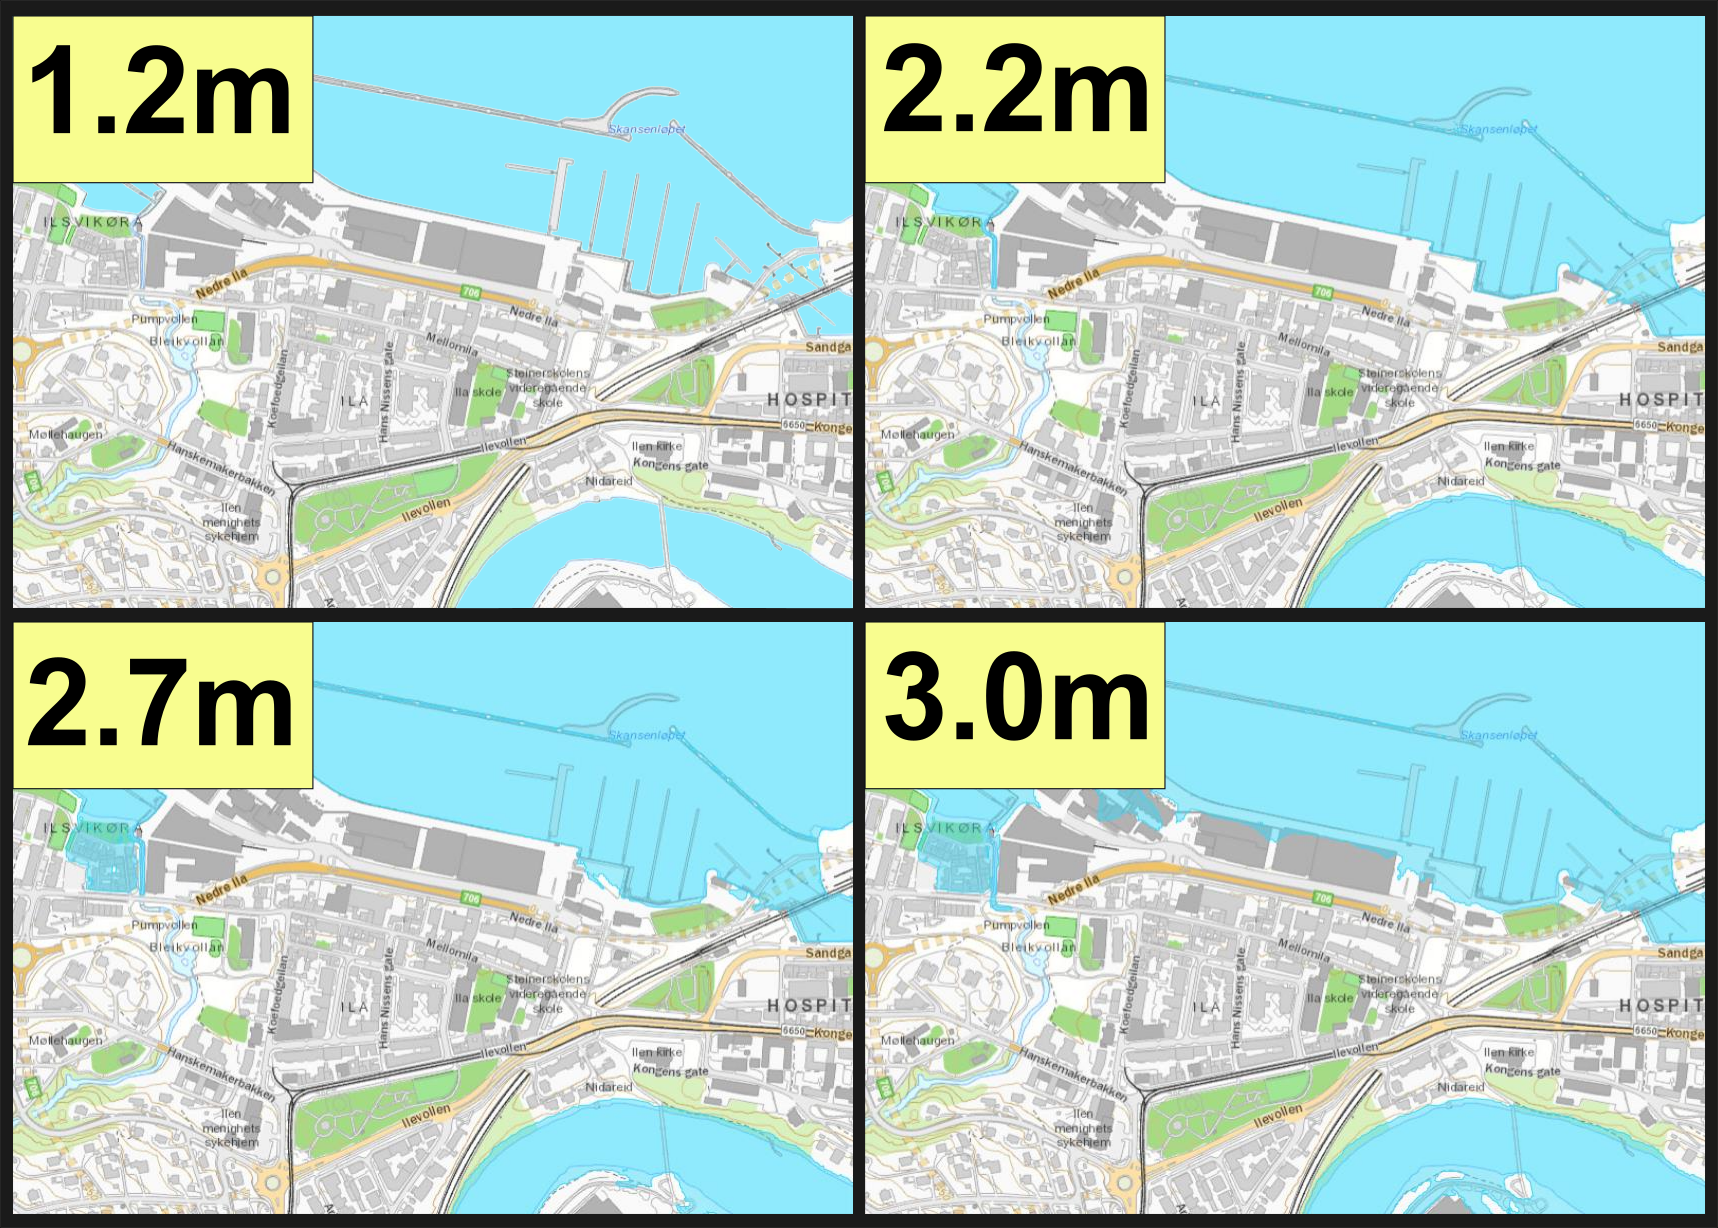
\includegraphics[width=16cm]{fig_sle/skansen-sle-num.png}
    \caption{Projected SLEs for Skansen}{These were created using \cite{kartverket_se_2021}, ArcGIS Pro and Inkscape. }
    \label{fig:sle_skansen_num}
\end{figure}

\begin{figure}[H]
    \centering
    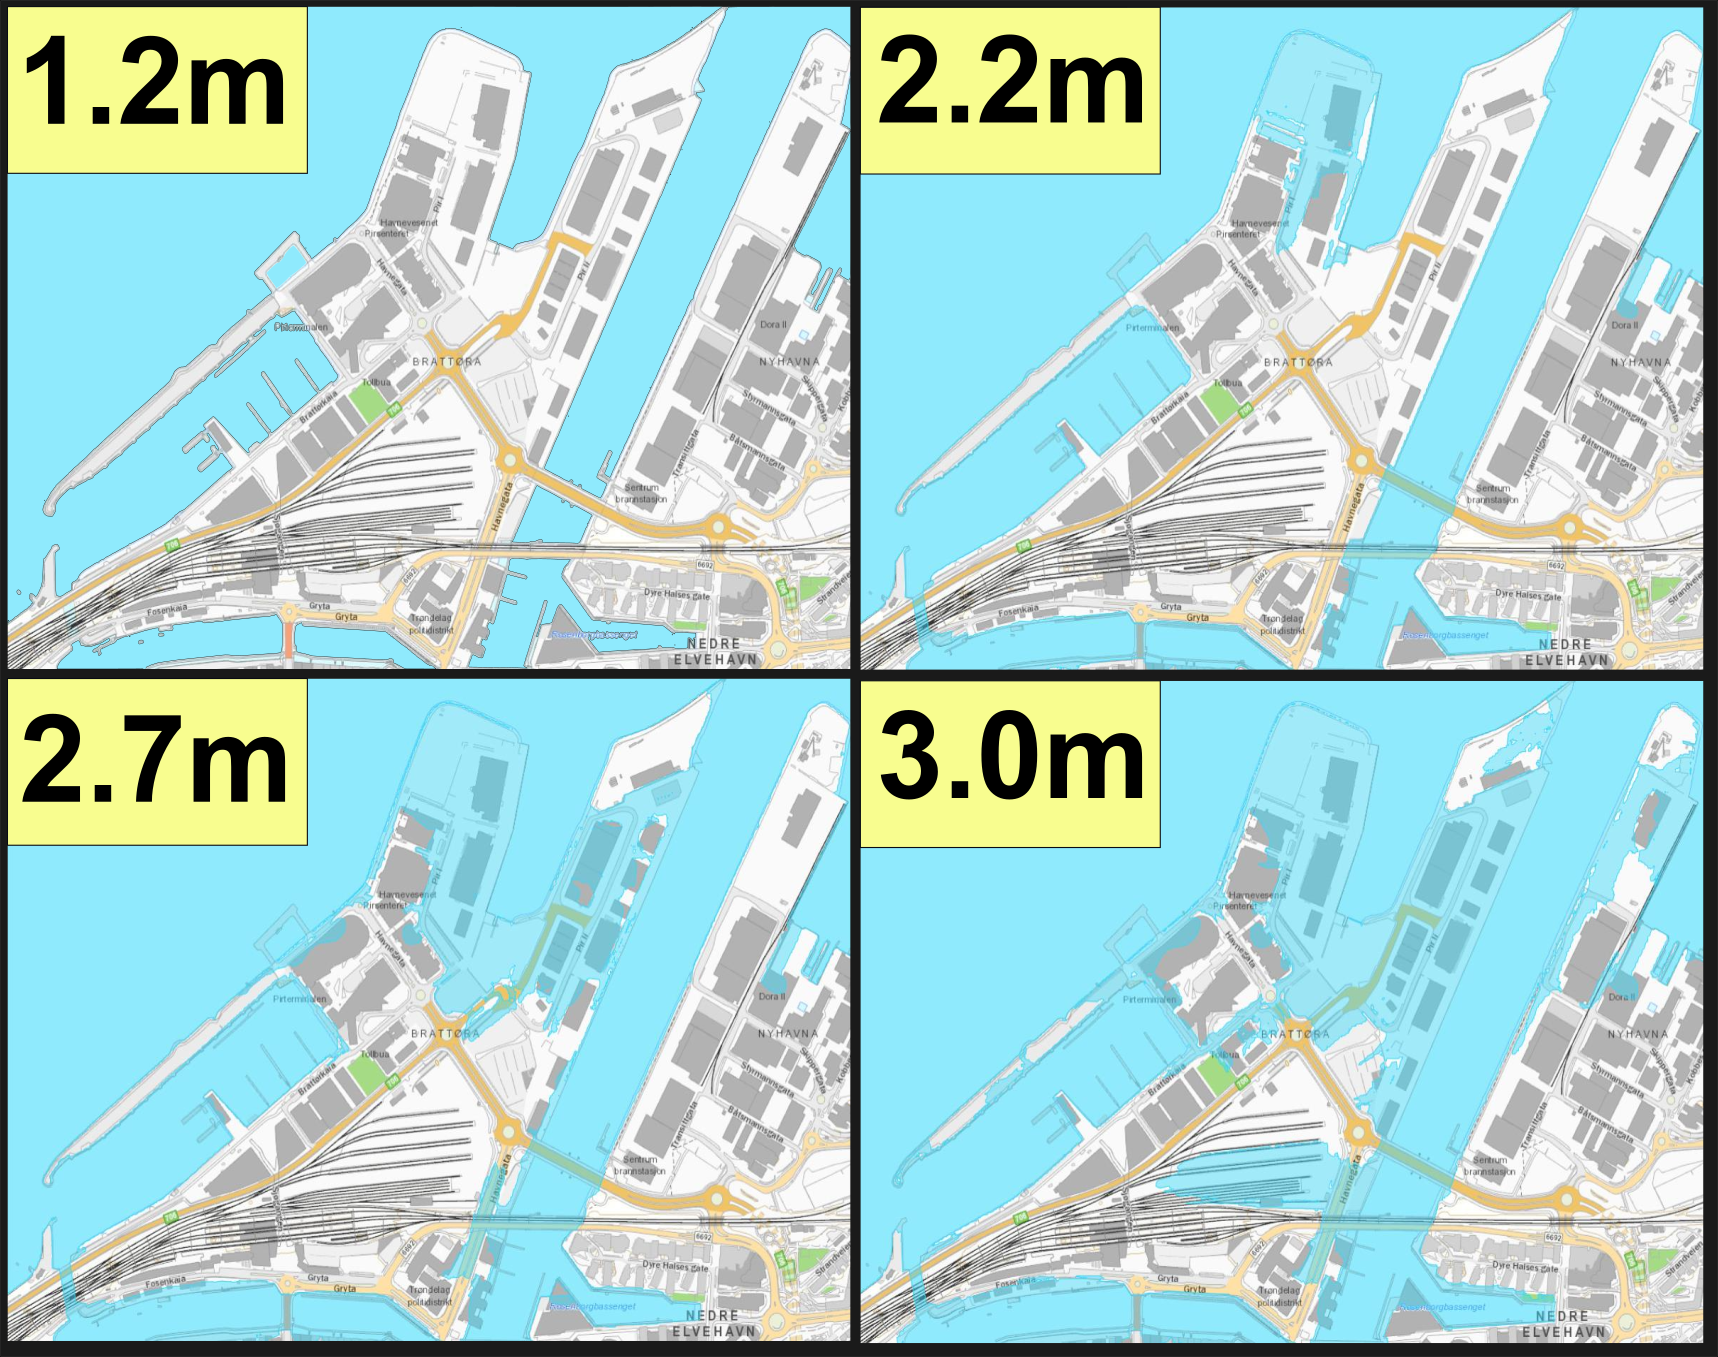
\includegraphics[width=16cm]{fig_sle/brattora-sle-num-bigger-boxes.png}
    \caption{Projected SLEs for Brattøra}{ These were created using \cite{kartverket_se_2021}, ArcGIS Pro and Inkscape.  }
    \label{fig:sle_brattora_num}
\end{figure}

\begin{figure}[H]
    \centering
    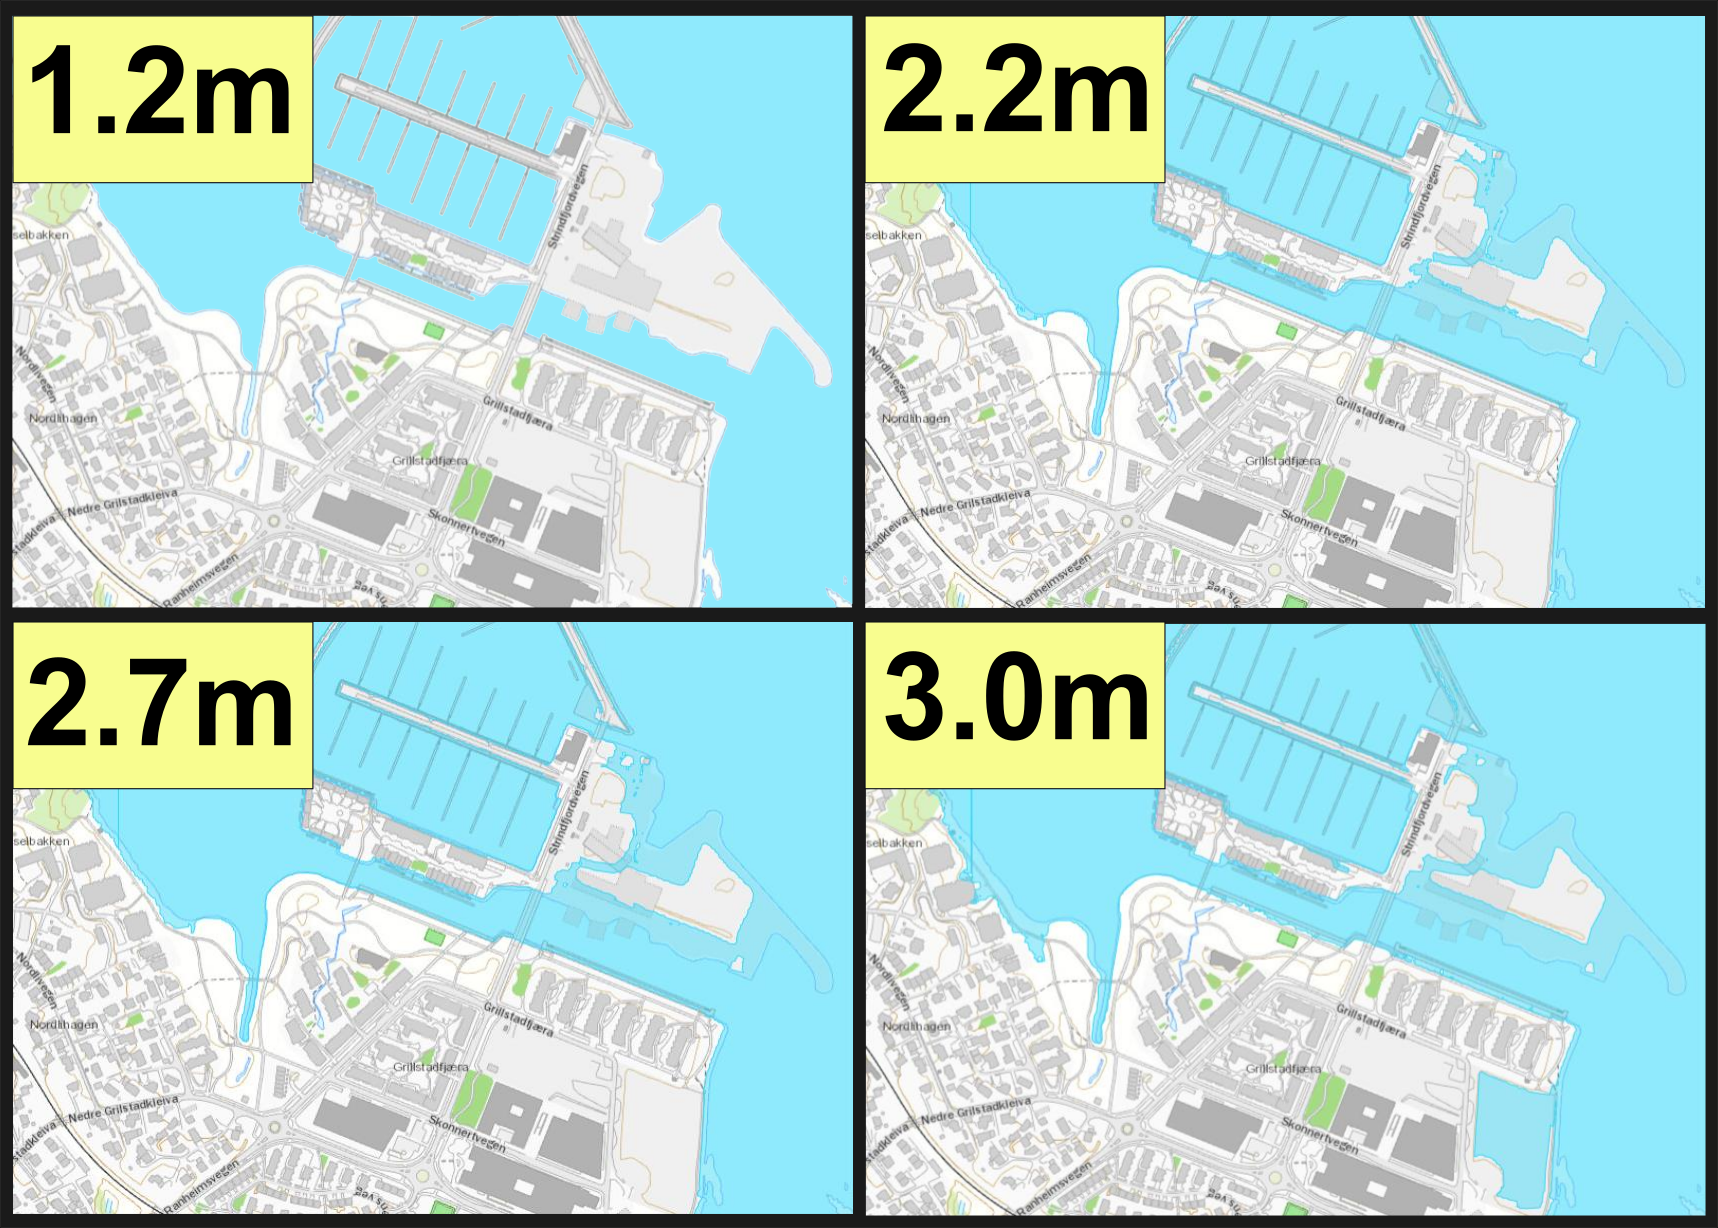
\includegraphics[width=16cm]{fig_sle/grillstad-sle-num.png}
    \caption{Projected SLEs for Skansen}{ These were created using \cite{kartverket_se_2021}, ArcGIS Pro and Inkscape.  }
    \label{fig:sle_grillstad_num}
\end{figure}

\begin{figure}[H]
    \centering
    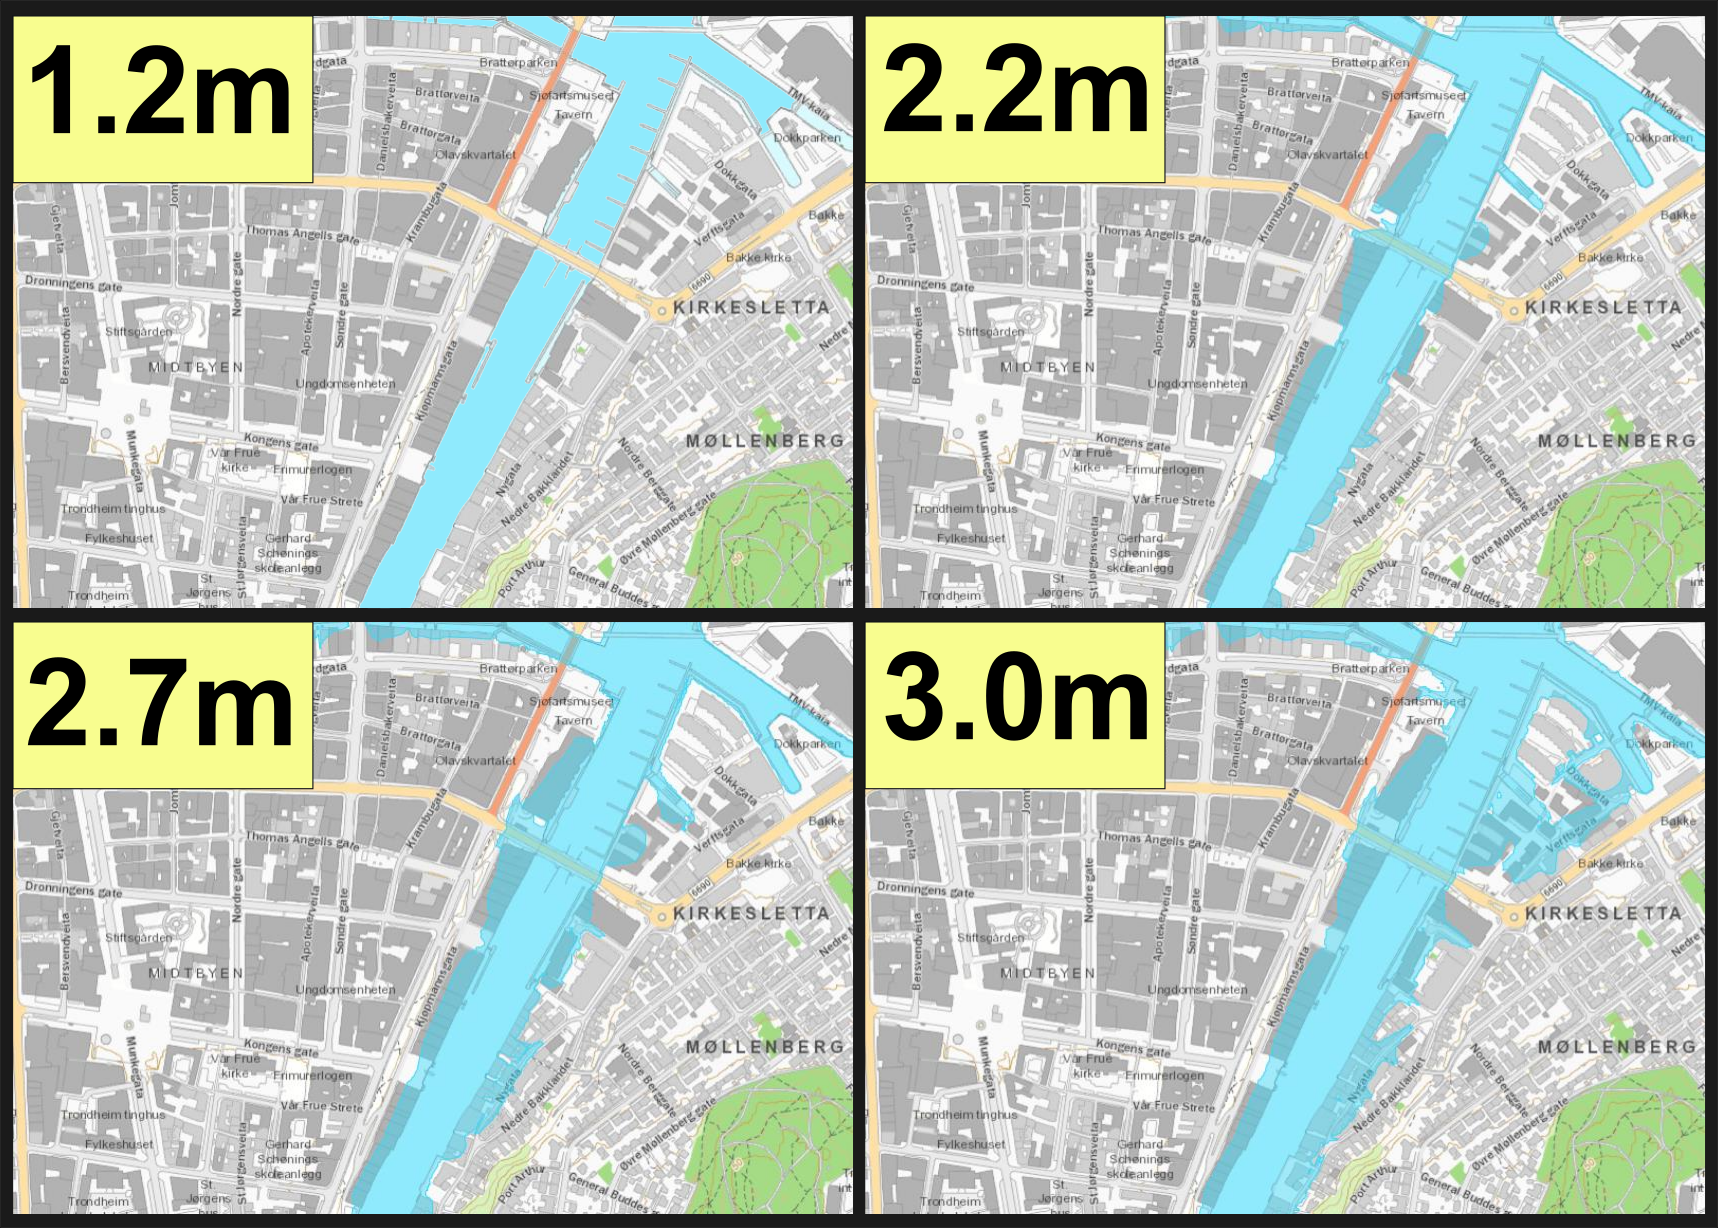
\includegraphics[width=16cm]{fig_sle/nidelva-sle-num.png}
    \caption{Projected SLEs for Skansen}{These were created using \cite{kartverket_se_2021}, ArcGIS Pro and Inkscape. }
    \label{fig:sle_nidelva_num}
\end{figure}

 Bridges were not well included in the original models; as all bridges were marked as being flooded at every water level, which was not in line with the numerical values. The bridges in these maps have been adjusted to more accurately match the SLEs represented. The differing heights represent different potential events,  as described with the edited photographs shown in section \ref{visual-simulations}. 

\section{Technological Systems Resilience}
Distinguishing technological and natural systems can be difficult in a landscape which has been actively shaped by its population for as long as Trondheim. Trondheim has been populated since the stone age and a major population site for over 1000 years (\cite{sjavik_z_2010}). For this thesis the understanding of technological system resilience focuses upon infrastructure in the four study sites, especially the location of buildings and roads. Of course how this infrastructure is built is of great importance to whether a speedy return to normality is possible after a sea level extreme event. Norway has strict building regulations, with additional rules about infrastructure in vulnerable locations (\cite{direktoratet_for_byggkvalitet_direktoratet_2016}). Yet, even very well-designed infrastructure will still be impacted if flooded. Impacts range from the obvious prevention of use during flooding, to post-event clean up and the wear and damage which can occur due to  erosion around building foundations, wave abrasion and salt-water damage.
\paragraph{}
Table ~\ref{table:building-impact-sle} displays the number of buildings which are likely to be impacted during different SLEs in Trondheim. This was modelled by \cite{kartverket_se_2021} and was the base of later water level simulations as used in this project. Importantly, the models from \cite{kartverket_se_2021} are more localised than previous models of SLEs in Norway.

\begin{table}[H]
    \centering
    \begin{tabular}{|l|l|l|l|l|}
    \hline
        \textbf{projected SLEs }& \textbf{No. Buildings}  & ~ & ~ & ~ \\ \hline
        ~ & Private & Private & Public  & Critical  \\ \newline
        ~ & Buildings & Businesses & Buildings & Buildings \\ \hline        
        20 years return height 2022 & 160 & 77 & 10 & 0 \\ \hline
        200 years return height 2022 & 214 & 87 & 10 & 0 \\ \hline
        1000 years return height 2022 & 242 & 104 & 14 & 0 \\ \hline
        Flooded 2090 & 66 & 51 & 8 & 0 \\ \hline
        20-years return height 2090 & 264 & 119 & 17 & 1 \\ \hline
        200-years return height  2090 & 308 & 136 & 24 & 1 \\ \hline
        1000-years return height  2090 & 332 & 148 & 26 & 1 \\ \hline
        1m sea level rise & 127 & 64 & 9 & 0 \\ \hline
        2m sea level rise & 343 & 155 & 29 & 1 \\ \hline
        3m sea level rise & 584 & 285 & 55 & 3 \\ \hline
        4m sea level rise & 752 & 335 & 70 & 5 \\ \hline
        5m sea level rise & 1023 & 402 & 77 & 8 \\ \hline
    \end{tabular}
    \caption{Impact of SLEs to Buildings in Trondheim }{translated from \cite{kartverket_se_2021}. Critical building are those which are critical to the function of the community such as hospitals. Explanation of "years return height" is available in section \ref{theory-nature-tech-resilience} }
    \label{table:building-impact-sle}
\end{table}


Table ~\ref{table:building-impact-sle} shows that there is currently some risk from SLEs to buildings in Trondheim, now and in the future. For example, the projected 20 years return height 2022 is expected to cause the flooding of 247 buildings in total. Additionally, the table shows the number of buildings projected to flood at different projected SLEs. The major contrast between the 20 years return height 2022 and the 20 years return height 2090 is that the water level is high enough to flood a critical building, such as hospitals. Flooding of a critical building would also occur at 2m sea level rise. It is projected by 2090 that 125 buildings will be continuously flooded.

%Theory --- important this is clear as possible
% first trial includes a lot of figures as it makes it clearer to me
\documentclass{article}
\usepackage{graphicx}

\begin{document}


\title{Theory}

\section{Key Terms}

\subsection{Citizen Science}
Words to define: 
•	Citizen Science \cite{tweddle_guide_2012}
Why citizen science for this project 

\subsection{Stakeholders}

The stakeholders primarily considered during this project are the people who live commute or work in coastal Trondheim. This was decided using \cite{reed_stakeholder_nodate} as a back up for a very basic stakeholder analysis. Other stakeholders consdiered are people with attachment to the research sites as well as well as planners and policy makers. Creating a full understanding prior to research of who was a stakeholder was not a priority as the primary research method relies upon stakeholders to self identify as those who decided to take part in this research. However targeting of subjects utilising the decided upon stakeholders was done. 

The stakeholders identity is a key part of the research. The nature of stakeholder participation during this project was limited to communication and consultation according to Rowe and Frower 2000 in \cite{reed_stakeholder_nodate}. How these stakeholders are categorised is top down as community membership of certain groups were targeted with the ability to identify as these groups during the survey. However there was also bottom up stakeholder identification as subjects could write in which groups they felt part of, beyond those decided on during the project design. Stakeholder theory is not one of the lenses in which these results are analysed, however an understanding of what and who the stakeholders are in the changing impacts of sea level extremes in Trondheim was essential to allow the assessment of local knowledge and awareness. 

\subsection{Local Knowledge}

what is local knowledge
why is it important for resilience
awareness of risk as a facet of local knowledge 
 Awareness (vs knowledge vs perception)

 %insert graphic to be the same width as the text
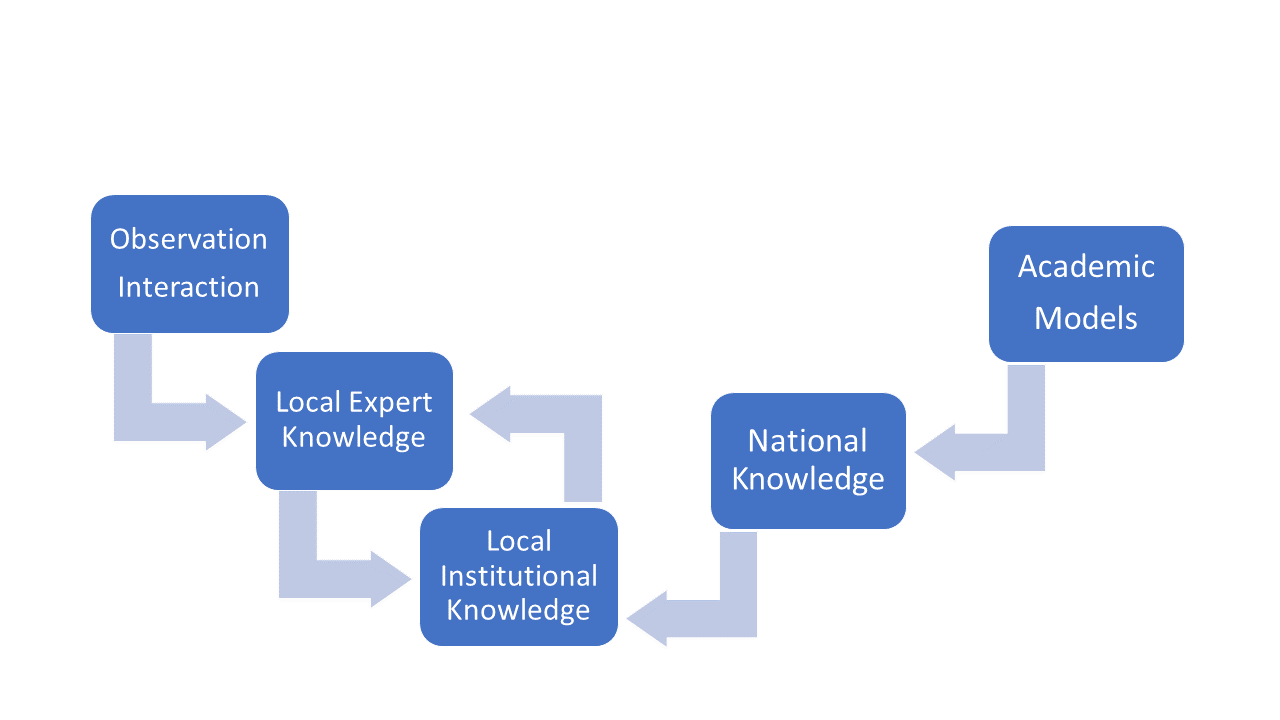
\includegraphics[width=1\textwidth]{fig_theory/local knowledge accumulation.png}

%create figure descriptor in a simple box 
\begin{frame}{Figure Local Knowledge accumulation.}
\end{frame}
 
\subsection{Vulnerability}
Vulnerability of a place is impacted by many broad influences including Local Knowledge 
Vulnerability – Lujala / Lein / Setten 



\subsection{Space,Time, Place} 
To understand resilience we must ask resilience: for whom; of what; to what; of where; how and when \cite{cutter_community_2020}, \cite{moser_turbulent_2019}. Resilience is temporally and spatially dynamic \cite{cutter_community_2020}. Hence a basic description of what is meant here by space, time and place is necessary. The conceptualisation used here is inline with \cite{massey_for_2005}, where space is the dimension of simultaneity and is part of space-time. In this view space is considered as the dimension of things being and importantly occurring at the same time. In contrast time is considered as things occurring one after the other. This conceptualisation of space-time is relevant for private, public and even virtual spaces and gives room for the social networks that operate within these spaces \cite{massey_for_2005} \cite{allen_rethinking_1998}.

The four chosen research places are created upon a combination of public and private space. The edge of the water itself is usually considered public space *REF* but there is also space allocated to specific groups which can create feelings of in-place vs out-of-place. Place is considered as an assemblage of traces. These traces range from the historical and global to the local and present and it is these combinations of traces which combine to make these places \cite{anderson_understanding_2015} \cite{massey_for_2005}. As well as explicit group membership the traces of place influence who can feel in-place and what is culturally and legally allowable uses of the places \cite{anderson_understanding_2015}. The four research sites include a wide demographic users of who can be considered in-place, but the power relationships and the in-place members affect the resilience of the location. 

\subsection{Awareness}
To understand the current resilience of a place requires an understanding of the awareness of the people who interact with and define the place. An individual’s ability to rank their level of awareness about a subject is a long investigated and debated topic *ref*. It is generally preferable to allow them to display their level of awareness rather than ask them on a sliding scale how aware they are. This is especially important when trying to explore knowledge which may have previously been seen as lesser.

To determine awareness level three questions were set in the survey used. These questions were designed to be simple and quick to answer in a format which would allow the author to analyse awareness about sea level extremes in the present and future along with general knowledge of the sea. Awareness about tide level, current risk of storm surges, past resilience to storm surges and future resilience to storm surges was investigated. Further information of how different question techniques and formats were trialled, and the influence of the decided questions format can be found in the Discussion section.

The choice which format method to use while asking about sea level changes is likely to have an influence on how participants perceive this change. For example considering change as metres in height vs area of land influenced may results in different perceptions of the changing risks and potential impacts.  By sticking firmly in the realm of historical fact and scientific models with these questions there has been an attempt to investigate awareness of SLEs rather than perception. 
%insert graphic to be the same width as the text
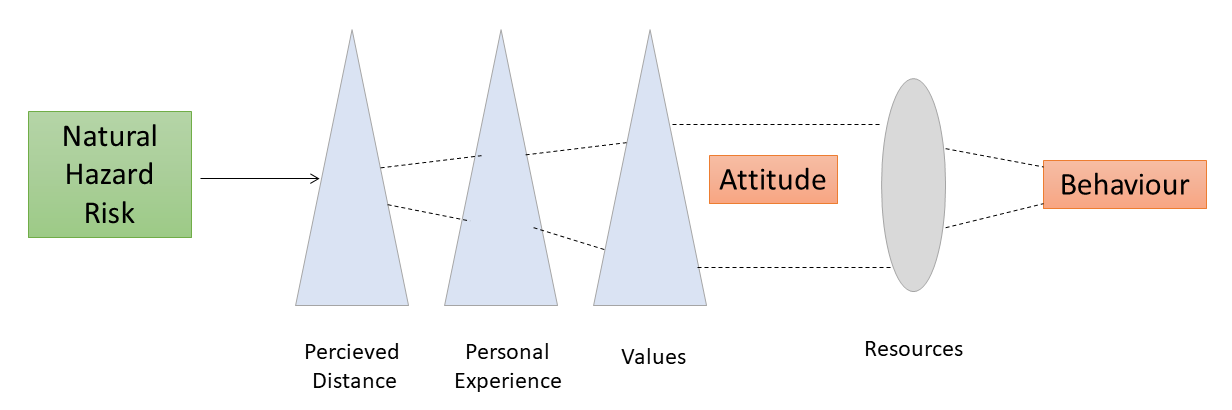
\includegraphics[width=1\textwidth]{fig_theory/awareness lujala and whitmarsh.png}

%create figure descriptor in a simple box 
\begin{frame}{Awareness of Natural Hazard Risk to behaviour pipeline based of \cite{lujala_climate_2015}\cite{whitmarsh_are_2008}.}
\end{frame}

Resilience is impacted by the behaviour of those who are potentiall impacted by the potential hazard. Awareness is influenced by many factors. Fig ** above is based on \cite{whitmarsh_are_2008} and \cite{lujala_climate_2015} . Where the green box labelled "Natural Hazard Risk" is the awareness of the individual. The three triangles are the prsims of "percieved distance", "personal experience" and "values" which have a signigicant impact on how this awareness is manifested as attitude to the natural hazard risk. This "attitude" is then put through the lens of "resources" before influencing the behaviour of the individual. 

Of course people's information in, to thought, to behaviour process are much more complicated than the visualisation above, but it is helpful to considered these prisms and lens when attempting to understand why individuals behave as they do. There is assumptions that those with higher levels of awareness about risks are more likely to have certain attitudes and in turn certain behaviours, but this is not always the case. 
*MORE ABOUT*\cite{lujala_climate_2015}  Awareness of the changing tides and risk of storm surges is considered here as an aspect of local knowledge. 

\subsection{Local Knowledge}
Awareness of the hazard investigated from sea level extremes is just one aspect of local knowledge which can have significant impacts on resilience. 

Formation of local knowledge "what we know anyway" \cite{setten_we_2019}




\section{Resilience}
Resilience - cutter

\section{Projecting Resilience of Place}
Key theories:
•	DROP cutter
•	Social systems as what defines resilience
•	Projected resilience as dynamic process which influences outcomes (i.e. resilience as measured post disaster). 
•	Cutter et al 2008
•	Cutter 2020 
•	Moser et al 2019 

\section{Defining Resilience} 
Resilience is here considered as the ability to return to normality as quickly as possible after disaster this is in line with (Cutter, 2019:Löw, 2019).

"present does not define future resilience, but it does influence it. Resilience as dynamic and dependent on 3 changing systems -natural, social and technological
" \cite{cutter_community_2020} views of resilience.

Sea Level Extremes can cause disaster, but this is not necessarily the case. A sea level extreme thus can be viewed as a possible disaster which is referred to here as an event. 

""Resilience is the ability of a social system to respond and recover from disasters and includes those inherent conditions that allow the system to absorb impacts and cope with an event, as well as post-event, adaptive processes that facilitate the ability of the social system to re-organize, change, and learn in response to a threat" "Vulnerability is the pre-event, inherent characteristics or qualities of social systems that create the potential for harm. Vulnerability is a function of the exposure (who or what is at risk) and sensitivity of system (the degree to which people and places can beharmed" " \cite{cutter_place-based_2008}

%insert graphic and rezise 
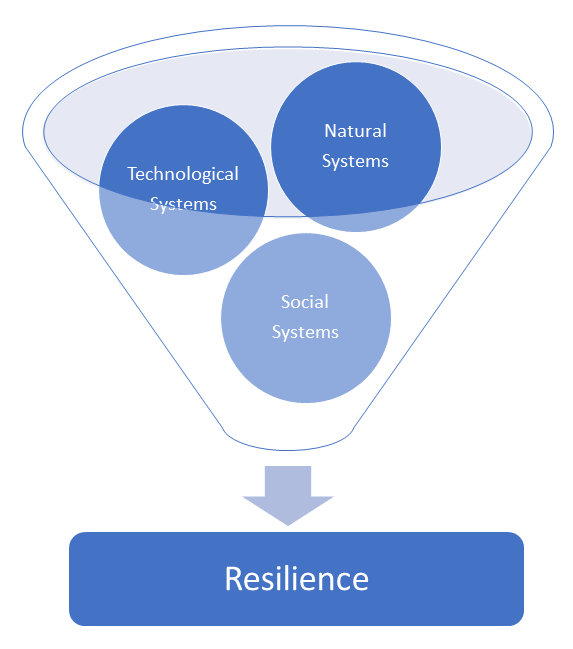
\includegraphics[scale=0.5]{fig_theory/resilience model .png}

%insert graphic to be the same width as the text
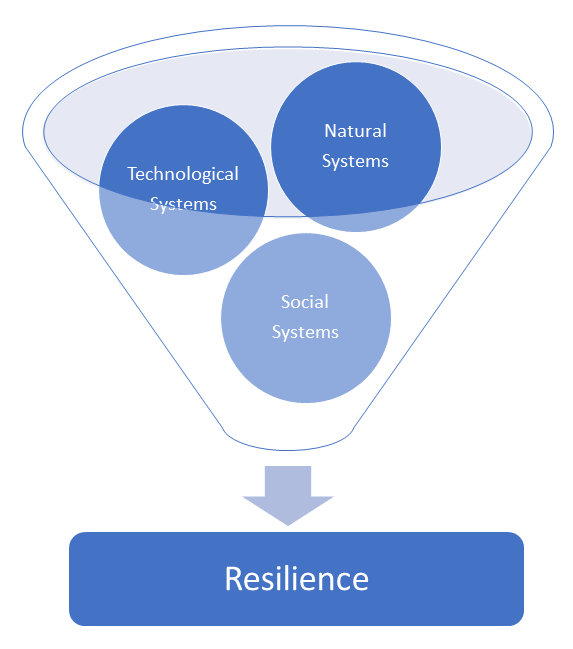
\includegraphics[width=1\textwidth]{fig_theory/resilience model .png}

%create figure descriptor in a simple box 
\begin{frame}{Figure Model of Projected Resilience and the systems involved in its creation }
\end{frame}

Resilience is an ongoing dynamic process. When discussing resilience in this thesis we are discussing projected resilience. Hence what is the projected ability to return to normality as quickly as possible after an sea level extreme event. 
 
Focusing on place based resilience and including community and institutions under the social system aspect
Rather than using community resilience in its place-based approach as commonly conceptualised in Norway both in National and local policy documents and by “layperson” (Räsänen et al 2020). Especially as highlighted by (Räsänen et al 2020) that how useful current place -based metirics are for measuring community resilience and that there is need for other techniques. Hence don’t ignore community but place it under social systems. 
•	Place based resilience vs community resilience
•	What they are why they differ and why I am using place based resilience


\subsection{Social Systems impacting Resilience}
community resilience as key aspect of social systems
local knowledge is part of that

\subsection{Technological Systems}

\subsection{Natural Systems }
SLE = WAVE + SEA LEVEL + TIDE + STORM SURGES + land movement

Storm Surge
“Storm surges are high water levels in the sea that occur during spring tides in combination with special weather conditions such as low air pressure and strong onshore winds.” According to the kommune (Einar Aassved Hanssen, Marianne Langedal, 2013) – stormflo = storm surge
“Safety against floods and storm surges is regulated by safety classes based on the
largest nominal annual probability. Flood sizes are usually stated with a number of
years of repetition intervals. The recurrence interval indicates how often a flood or
storm surge of the same magnitude occurs on average over many long years. A flood
with a recurrence interval of 200 years, also called a 200-year flood, occurs on average
every 200 years. Each year, the probability of a 200-year flood is equal to 1/200, ie 0.5 percent.
This does not exclude that one can get two 200-year floods at short intervals.
Calculation of recurrence intervals for floods and storm surges is based on historical
observations, and measurement of water flow or water level.”
Building technical regulations (TEK17) with guidance Chapter 7 Safety against natural stresses

\title{Sea Level Extremes}
%insert graphic to be the same width as the text
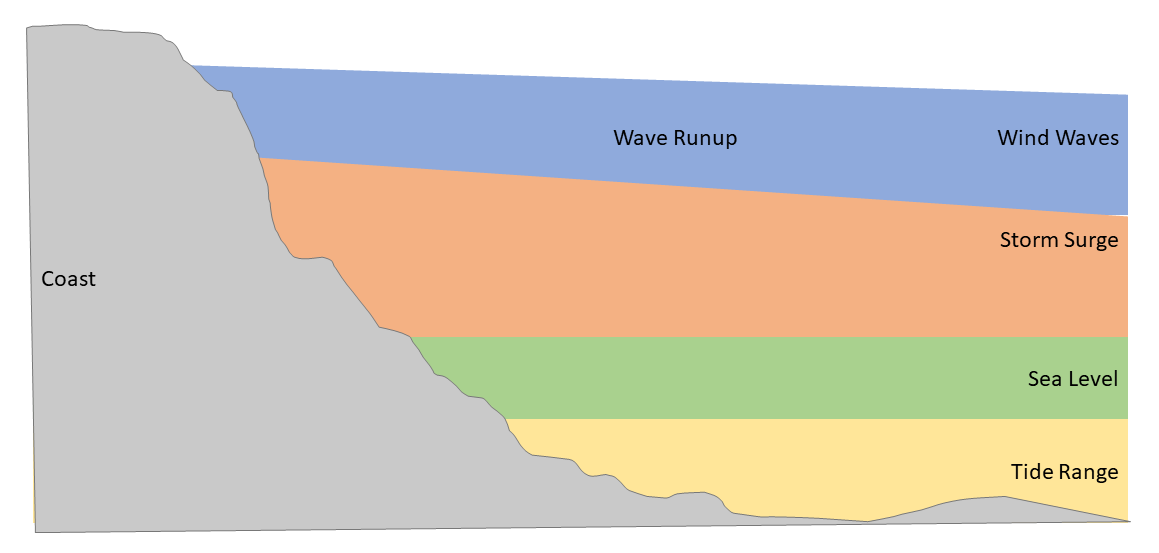
\includegraphics[width=1\textwidth]{fig_theory/sea level extremes.png}

%create figure descriptor in a simple box 
\begin{frame}{Figure The various aspects which combine to create extreme sea levels. Tide Range, Sea Level, Storm Surge, Waves due to the wind, Waves due to the run-up onto the coast.}

Sea Level extremes are due to the combination of various variables which for Trondheim's fjord can be impacted by the changing climate. 

\end{frame}


\end{document}
%automated figures
%Methodology section including data collection and data analysis technique
%no results or discussion here
%where the decisions made goes
%then discuss the decisions made in the discussion of framework

\chapter{Methodology}
To determine Trondheim's resilience to future SLEs requires an understanding of its technological, natural and social systems. Literature reviews of  municipality policies and planning permissions were carried out to determine the technological systems resilience. Natural systems resilience determination relied on research site observations and analysis of several  data-sets including: \cite{geonorge_stormflo_nodate} , \cite{kartverket_se_2021}, \cite{stormflo_database_stormflo_2021} and \cite{ipcc_sea_2021}. 
\paragraph{}
To determine Trondheim's social system resilience, data collection utilising an online survey was carried out. The purpose of this survey included gathering data about local knowledge of past, present and future SLEs. To improve the design of this survey, a pilot survey and focus group were first carried out.  

\section{Data Sources} \label{data-sources}
 Natural systems resilience determination relied on research site observations and analysis of several  data-sets including: \cite{geonorge_stormflo_nodate} , \cite{kartverket_se_2021}, \cite{stormflo_database_stormflo_2021} and \cite{ipcc_sea_2021}. 

 
\section{Data Collection} \label{data-collection}

Data collection for this study comprised two parts.  The first part involved conducting literature reviews and collecting models of sea level rise and SLEs. The aim was to create a realistic visualisation of SLEs in Trondheim between 1950 and 2100 to utilise in discussion of awareness of SLEs. 
\paragraph{}

The second was an online survey conducted in the summer of 2022 drawing from a pilot survey and focus group conducted earlier in the year. The aim was to explore subjects' experience, awareness and information access with respect to SLEs and climate change. Subjects were recruited via social media, email and posters placed in the four study areas in locations where people wait, for example, at a train station. The survey was designed to take under five minutes to maximise responses. Stakeholders targeted were those with direct experience of Trondheim’s coast in the four research sites – Brattøra, Skansen, Nidelva and Grillstad. These locations were chosen after non-intrusive, naturalistic, participant observation of coastal public places (\cite{del_casino_social_2009}) along all populated areas of Trondheim’s coast. In other words the researcher systematically sat and observed the busiest, public, coastal locations and noted who passed by to make sure that all demographics in Trondheim regularly attended these locations without influencing the variables in this place (\cite{del_casino_social_2009}). The observable characteristic used to determine physical vulnerability is the ability to be flooded due to SLEs. Within this research, this was determined from direct observation of the research sites combined with models from \cite{kartverket_se_2020} and planning documents focusing on impact of storm surges (\cite{miljoenheten_og_byplankontoret_trondheim_kommune_9-notat-om-havnivastigning-og-stormflo---hensyn-i-arealplanlegging-nyhavnapdf_2020}). The city of Trondheim was selected due to the potential to utilise researcher's personal network and due to restriction surrounding COVID-19 pandemic. The individual research sites were chosen due to their high throughput of all demographics and perceived physical vulnerability.

\paragraph{}
To determine awareness level, five questions were set in the research survey. These questions were designed to be simple and quick to answer in a format that would allow the researcher to analyse awareness around SLEs in the present and future along with general knowledge, of the sea. Awareness about tide level, current risk of storm surges, past resilience to storm surges and future resilience to storm surges was investigated. Further information about how different question techniques and formats were trialled, and the influence of the decided questions format can be found in the Discussion.



\section{Communication Design} \label{com-design}

When utilising citizen science, communication style is very important. This section details the various methods used to reach subjects and encourage them to participate. Accessibility, trust and legitimacy are important attributes with all citizen science, but even more so when investigating subjects with a potential emotional impact (\cite{tweddle_guide_2012}). A simulated image which shows a place a participant cares about as being impacted by a SLEs could result in a strong emotional impact. If this is not handled carefully, this could turn the participant away from the survey and similar research.
\paragraph{}

To reach participants, the researcher's personal network was used, along with A4 posters, social media and emails to relevant organisations and employers. Fifty posters were displayed across the 4 research sites concentrating on areas where people gather, such as park benches and bus stops. Relevant permission was granted for each poster. The posters directed participants to a website containing details about the thesis and links to surveys on each research site.
\paragraph{}

The Web Accessibility Guidelines (\cite{henry_web_2022}) and Story Map Accessible Design Principles (\cite{todd_liz_getting_nodate}) were actively used  as guides for the creation of the website and online surveys, particularly their descriptions of high standards of visual communication and accessibility using different kinds of technology. For the text on the website and online survey,  Principles for effective communication and public engagement on	climate change: A Handbook for IPCC authors (\cite{corner_a_principles_2018}) was consulted. While not written for citizen science, its advice for discussing climate change and how to connect with people on these subjects is useful. 
\paragraph{}

The design principles followed in this study can be summarised as:
\begin{itemize}
    \item Make it as easy as possible to participate
    \item Utilize personal brand to enhance connection and trust
    \item Be succinct
\end{itemize}
\paragraph{}
These were developed from the guidelines mentioned above plus the researcher's previous experience working in communications, including training in visual communication. To enhance legitimacy, the results of this thesis will be shared with interested subjects via a website (https://aamccormack12.wixsite.com/sealevelextremes).
\paragraph{}
Example emails, social media posts and the poster used to access subjects are in Appendix B. The full survey in Norwegian and English is also included to demonstrate how the communication guidelines were implemented. Attempts were made to keep both the English and Norwegian survey as close as possible to allow for easy comparison. However, direct translation is not always possible and the nuance and implication of word choices can have significant impact on the results. This was minimised by the researched writing both surveys rather than relying on a translator. The researcher has English as a first language and Norwegian to a working standard. The surveys were checked by several individuals who have Norwegian as their first language along with a good understanding of the topic.


\section{Pilot Survey and Focus Group}

The pilot survey was conducted on the 21st and the 25th of March, 2022 with 14 subjects. The subjects were classed as highly aware as they all had familiarity with changing SLEs in Brattøra: they were either Natural Resources Masters students or members of Trondheim Kayak Club and they had the thesis presented by the researcher in advance of responding to the survey. The pilot subjects were asked seven questions, of which three were used in an attempt to determine the subjects' awareness of SLEs in Brattøra. Figure \ref{fig:brattora_2022_hightide}, \ref{fig:brattora_2090_stormsurge} and \ref{fig:brattora_2022_stormsurge} display the maps used when asking about the projected heights of SLEs.

\begin{figure} [H]
    \centering
    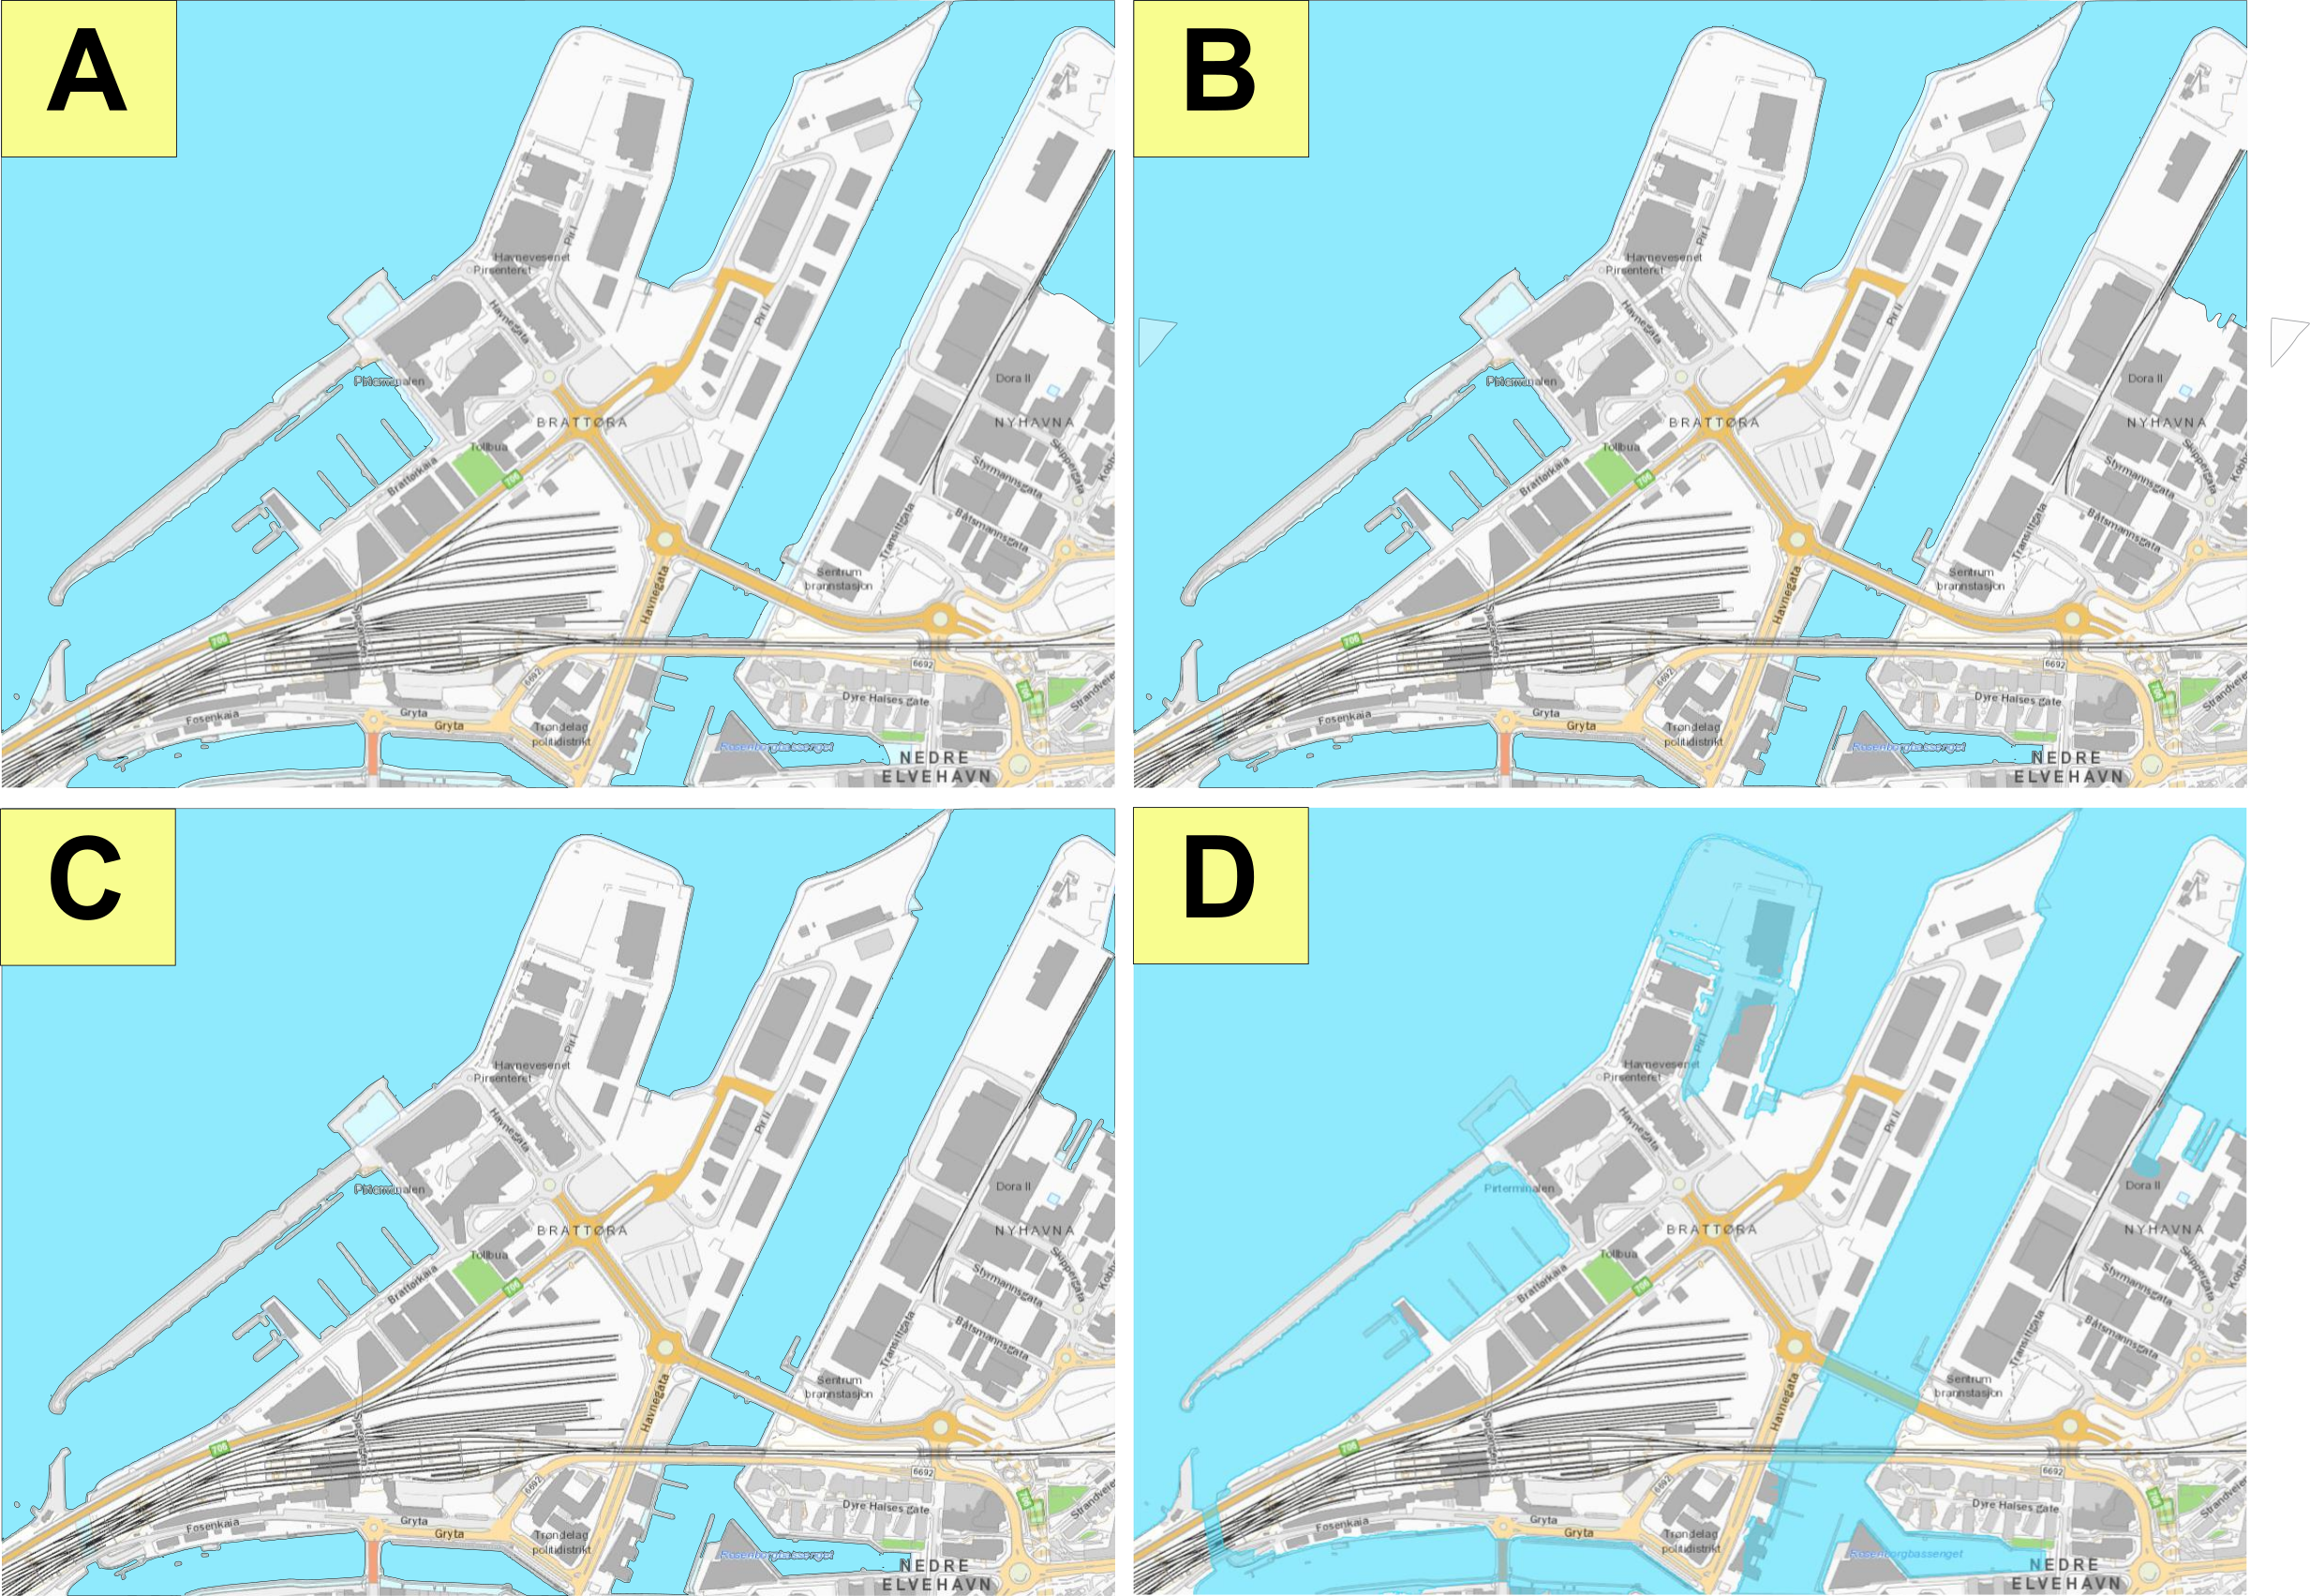
\includegraphics[width=16cm]{fig/brattora question on 2022 high tide quadrant.png}
    \caption{Pilot Survey Maps - Brattøra High tide}{For the question "Which image displays Brattøra's High tide?" -  This image contains four maps representing potential high tides in Brattøra. The map which matched models from \cite{kartverket_se_2021} is C. If subjects selected this response they were deemed aware of high tide in this place in the period 2022 to 2050. }
    \label{fig:brattora_2022_hightide}
\end{figure}

\begin{figure}[H]
    \centering
    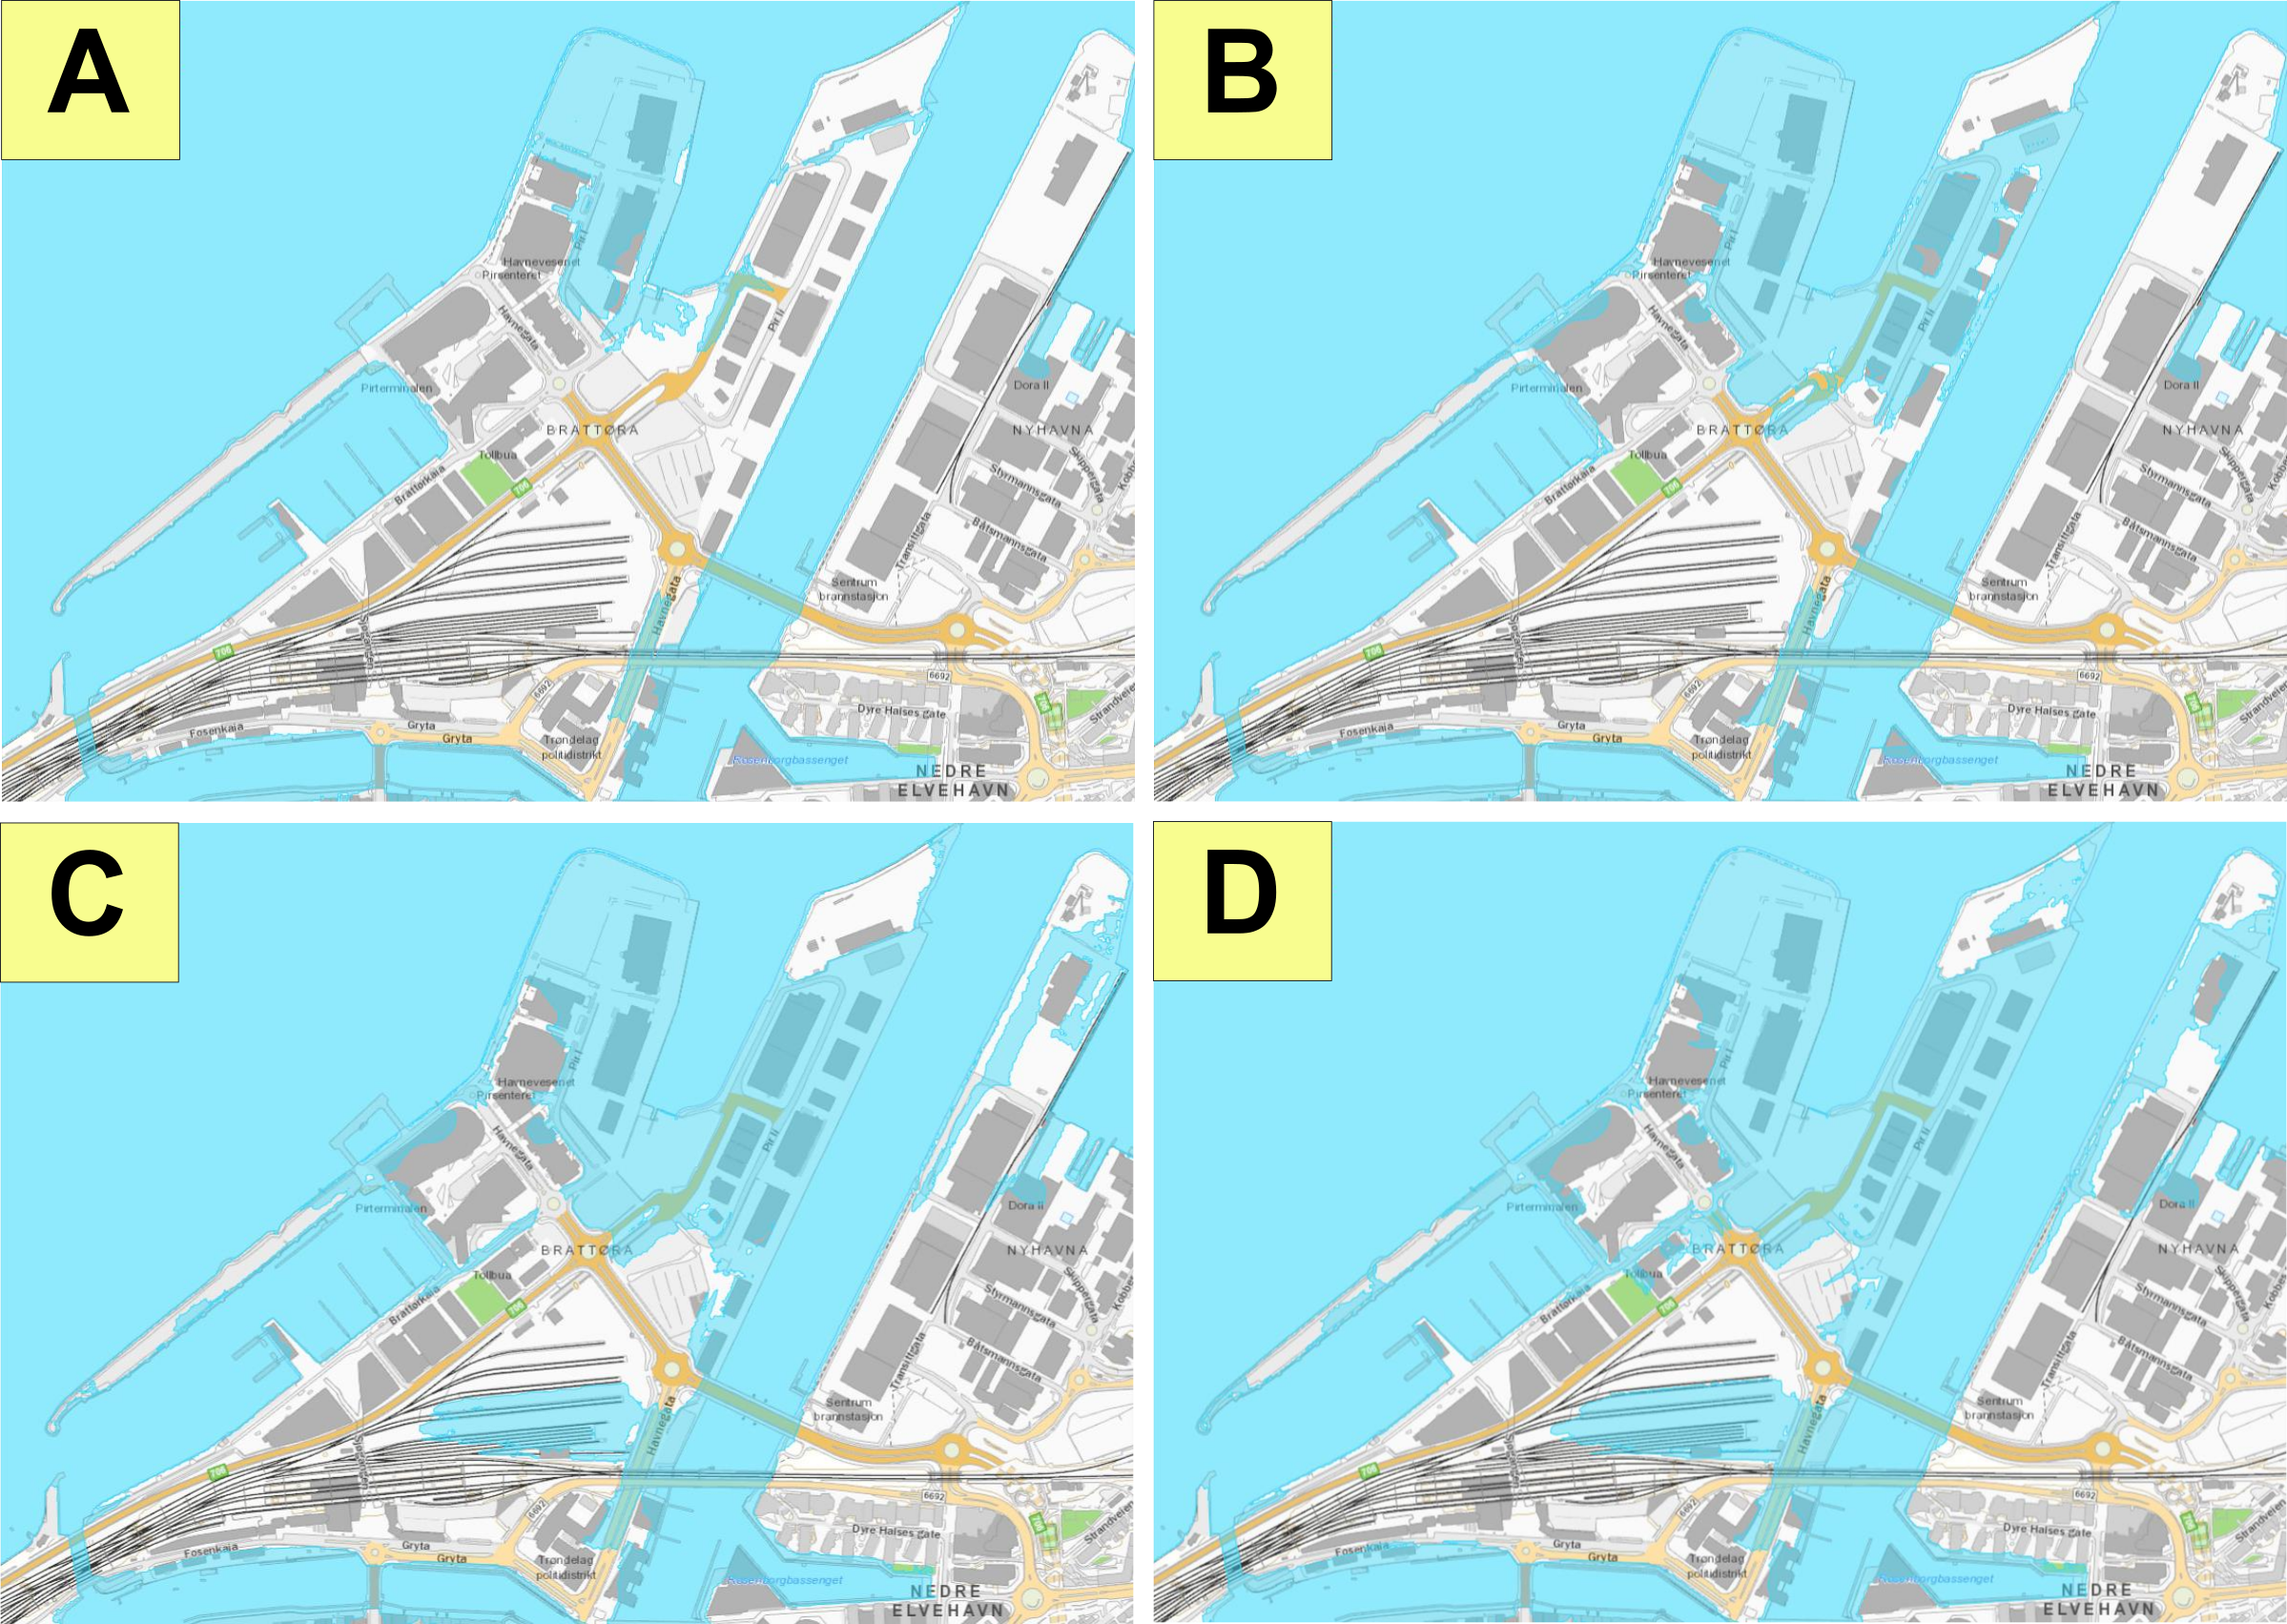
\includegraphics[width=16cm]{fig/brattora question on 2090 20 yr storm surge quadrant.png} 
    \caption{Pilot Survey Maps - Brattøra 20 year Storm Surge, 2090}{For the question "Which image displays Brattøra's 20 year storm surge in 2090?" - This image contains four maps representing potential heights which could be caused by the 20 year storm surge. The map which matched the models from \cite{kartverket_se_2021} is B.If subjects chose this response they were deemed aware of the 20 year storm surge in the period 2050 to 2100. }
    \label{fig:brattora_2090_stormsurge}
\end{figure}

\begin{figure}[H]
    \centering
    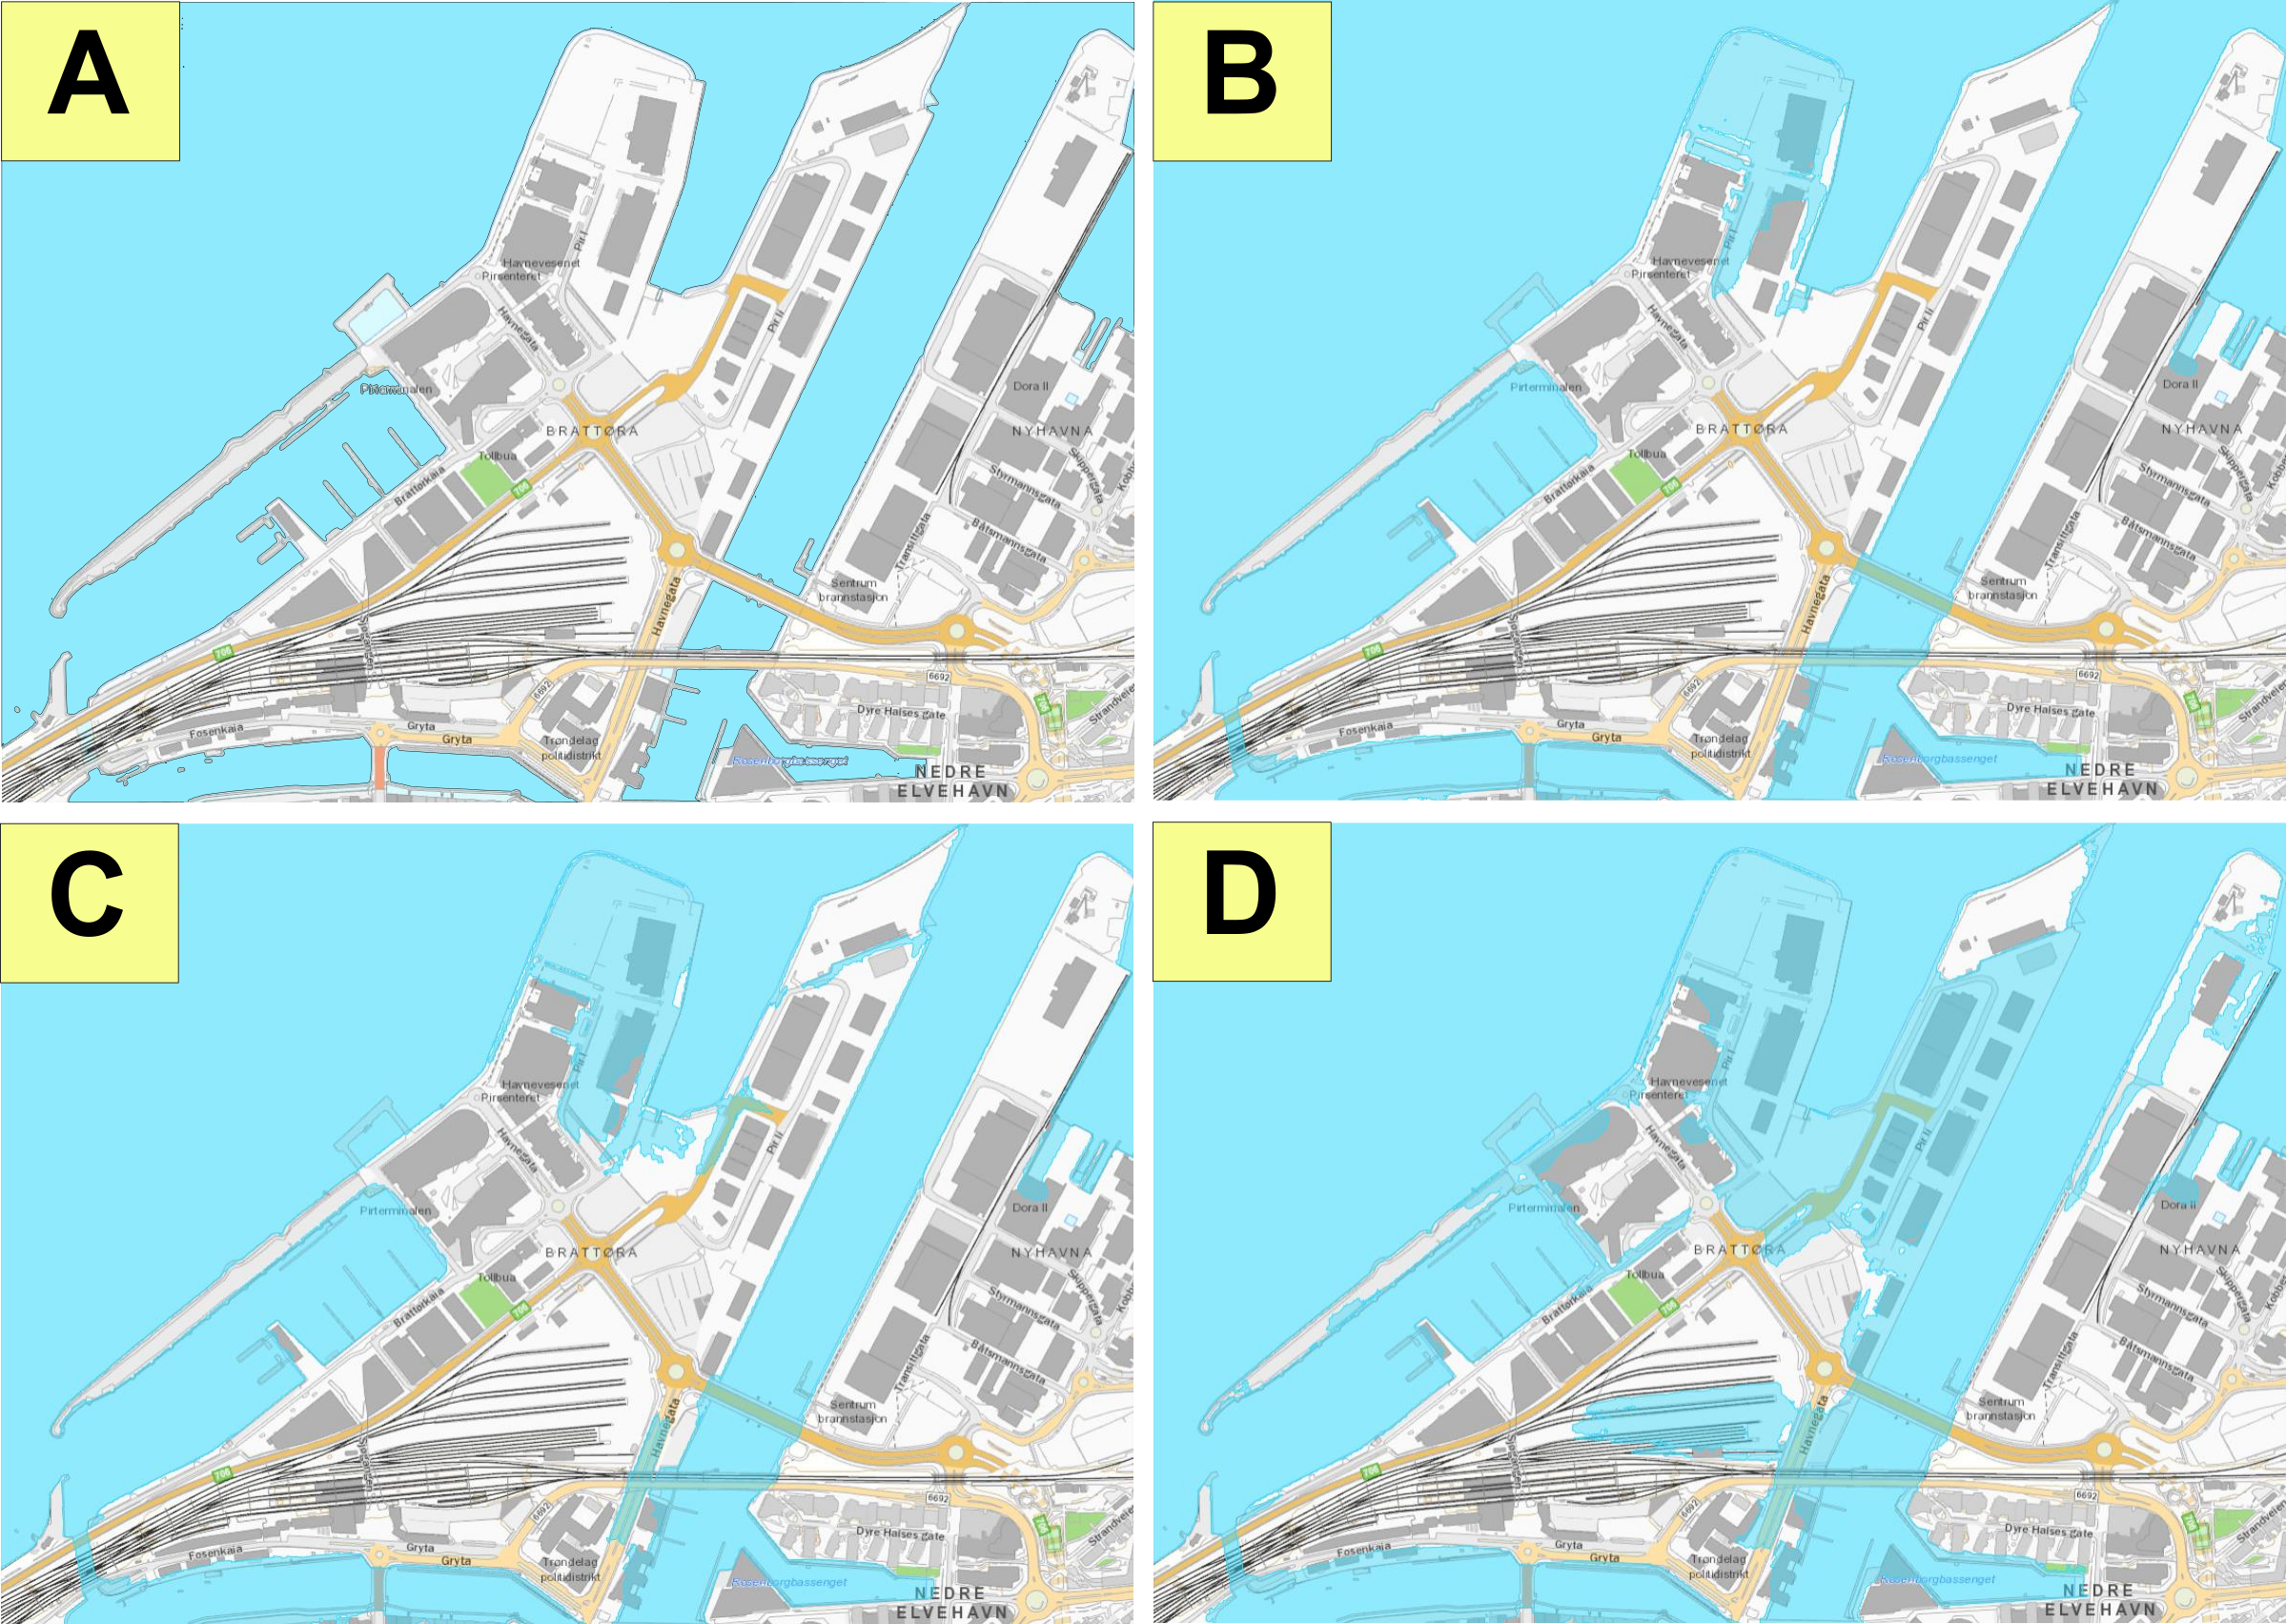
\includegraphics[width=16cm]{fig/brattora question on 2022 20 yr storm surge quadrant.png}
    \caption{Pilot Survey Maps - Brattøra 20 year Storm Surge, 2022}{For the question "Which image displays Brattøra's 20 year storm surge in 2022?" - This image contains four maps representing potential heights which could be caused by the 20 year storm surge. The map which matched the models from \cite{kartverket_se_2021} is B.If subjects chose this response they were deemed aware of the 20 year storm surge in the period 2022 to 2050.}
    \label{fig:brattora_2022_stormsurge}
\end{figure}

The difficulty the participants had answering these questions is discussed in the results. After this, a focus group was conducted with seven of the subjects from the pilot survey.  They were shown Figure \ref{fig:slide}, which was used to direct conversation. The purpose of the focus group was to determine whether the subjects truly had high levels of awareness about SLEs and if so, what prevented them from choosing the answer which corresponded with the models. The findings from the pilot survey and focus group were used to improve data collection methods. 

\begin{figure}[H]
    \centering
    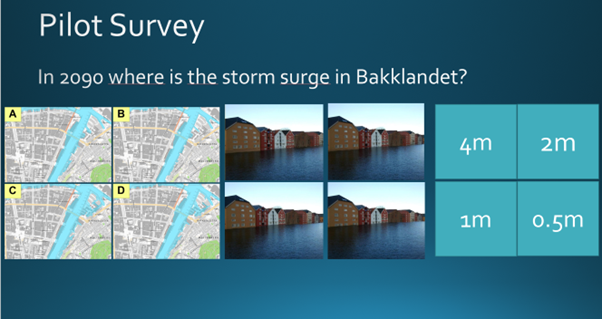
\includegraphics[width=1\textwidth]{fig_results/slide-pilot-survey.png}
    \caption{Focus Group Discussion Prompt Slide} {Displays the three options for communicating SLEs - maps, simulated photographs, numeric values}
    \label{fig:slide}
\end{figure}

\section{Digital Visualisation of SLEs}
To determine Trondheim's social resilience, a survey was carried out in the summer of 2022. A key aim of this survey was to determine subjects' awareness of changing SLEs.  Five questions were asked to gauge awareness. Three questions utilised visual simulations of SLEs for each of the research sites. These were created based on models from \cite{dsb_integrating-sea-level-rise-and-storm-surges--local-planningpdf_2017} and \cite{kartverket_se_2020}. Images were created for various potential SLEs at the chosen research sites. Photographs of the sites were taken to make understanding and editing as easy as possible. They were taken on a sunny day, minimising people and boats, while attempting to capture recognisable landmarks. The geo-location and timing of the photos were noted to allow for determination of the water height. Table \ref{tab:water_level_photo} below displays the water height of each of the original photographs. 
\paragraph{}

\begin{table}[H]
    \centering
    \begin{tabular}{|l|l|}
        \hline
     	\textbf{Research Site} & \textbf{Photograph water level (cm)} \\ \hline
            Grillstad & 50 \\ \hline
            Skansen & -23 \\ \hline
            Nidelva & -159 \\ \hline
            Brattøra	& -42 \\ \hline
    \end{tabular}
    \caption{Water levels as basis for simulated SLEs photographs}{Tables displays the water levels on the day and precise time of the photographs taken by the researcher to use as a base to apply simulated SLEs on top of. These values were determined from \cite{tides_high_2022} and included consideration of tide plus weather effects plus river levels}
    \label{tab:water_level_photo}
\end{table}
\paragraph{}

Using \cite{tides_high_2022} the base water level for each of the original photographs was determined. For Skansen, Grillstad and Brattøra, this meant combining the tides, plus weather effects. On most days, a calculation of Nidelva research site's water level would need to include the river level. However, time and day chosen was one with an observably low river level which allowed for this value to be excluded as water level was dominated by the tide at the time of the photo being taken.   
\paragraph{}

To these base water level photographs the simulated water levels could be digitally added. See figures \ref{fig:SLE-nidelva}, \ref{fig:SLE-brattora}, \ref{fig:SLE-grillstad}, \ref{fig:SLE-nidelva} within the section on Visual Simulations of SLEs in background chapter for the results of this process. Table \ref{tab:2022_sle_projections} and \ref{tab:2090_sle_projections} below show the SLEs and the associated water level with NN2000 as a reference point.  To be able to accurately add the simulated water levels to the images, the first step is to make sure that each of the photos included a reference height. These key features (bins, fences, permanent benches, windows) were measured using a tape measure to allow for simulated realignment of the water levels to particular heights. Perspective was an important consideration in the original photos. Having the coastline at an angle allowed for a more realistic image, but did complicate the photo editing. 

\begin{table}[h!]
    \centering
    \begin{tabular}{|l|l|l|l|l|l|}
    \hline
     Sea Level &   mean high  & mean high  & 20 year  & 200 year   & 1000 year  \\ \newline
     Extreme &  water neaps & water springs &  storm surge  & storm surge  &  storm surge  \\ \hline
       Height (cm) &  55 & 119 & 216 & 234 & 244 \\ \hline
    \end{tabular}
    \caption{2022 SLEs Projections }{\cite{kartverket_se_2020}}
    \label{tab:2022_sle_projections}
\end{table}

\begin{table}[h!]
    \centering
    \begin{tabular}{|l|l|l|l|l|}
    \hline
       Sea Level &  mean high & 20 year   & 200 year &  1000 year   \\ \newline
       Extreme & water springs &  storm surge  &  storm surge  &  storm surge  \\ \hline
       Height (cm) & 172 & 269 & 286 & 297 \\ \hline
    \end{tabular}
    \caption{2090 SLEs Projections}{ \cite{kartverket_se_2020}}
    \label{tab:2090_sle_projections}
\end{table}

Once the heights were calculated from the tables above, they were drawn onto the original photos using Inkscape. This new image was then used as the base layer when simulating SLEs. The original image was replicated twice using GIMP, GNU Image Manipulation Program, with a reduced opacity. The extra layer allowed for easier fixes during the next step. 
\paragraph{}
The top layer was then cut to leave only the water present in the image using the free select tool. If too much was cut the layer underneath could be used as a back up. After this, the handle transformation tool was used to define points. This layer was then aligned for each of the draw-upon water levels. Soft eraser tool was used to minimise oddities in the water created due to this movement. Dodge tool was used to darken below the water line to make the water line more distinct, as calm bright days were chosen, meaning the edge of the water was difficult to pin point on small screens. Finally, the clone tool was used to remove potential distractions, including seagulls and boats floating on the sea. The image was then exported as a JPEG. 

\paragraph{}
The final values and water levels used were rounded to 10cm for ease. The exported JPEGs were combined into grids and labelled for use in the survey. 

\section{Stakeholder Selection}
A subject's identity is a key part of the research. The nature of stakeholder participation during this thesis was limited to communication and consultation according to Rowe and Frower  (Rowe and Frower 2000 in \cite{reed_stakeholder_2008}). These stakeholders were selected in a predominately top down manner:  certain communities were targeted and individuals within these communities were asked to self identify (\cite{reed_stakeholder_2008}). However, there was also bottom up stakeholder identification as subjects could write in which communities they felt part of, beyond those decided on during the thesis design (\cite{reed_stakeholder_2008}). An understanding of what and who the stakeholders are in the changing impacts of SLEs in Trondheim was essential to allow the assessment of local knowledge and awareness. However stakeholder theory is not used as an analytical method.
\paragraph{}
The results will be published in an accessible form for those stakeholders who are interested. This is in line with the guidelines for citizen science set out by \cite{tweddle_guide_2012}. The data management plan and ethics guidance were created in line with \cite{nesh_guidelines_2022} and \cite{nsd_norsk_nodate}. 

\section{Data Analysis}
An exploratory data analysis was completed then non parametric hypothesis testing was conducted utilising RStudio. Histograms and Shapiro Tests were used to determine the distribution and scatter-plots were created to search for linear relationships. The results of the analysis were exported from R Studio to Microsoft Excel for ease of plotting.
\paragraph{}
The main survey comprised of 26 questions addressing awareness, memory of SLEs, interest levels in SLEs, community membership, information access, length of residence, attitudes as well as space to highlight other place-based risks. Linear regression and linear mixed effect models were originally planned as the main statistical analyses, but due to the lack of linearity, highlighted by the scatterplots in the exploratory analysis, non-parametric hypothesis testing was selected.


However, due to lack of linearity in original scatter-plots another method was also chosen. 153 responses were collected. 30 percent of respondents had no memory of SLEs in Trondheim with 70 percent having memory of one or more event. A third (50/153) remembered the most recent sea level extreme in February 2020. 
\paragraph{}
A non parametric hypothesis testing method was chosen due to the lack of linearity, and as the data was not normally distributed. Specifically the Kruskal Wallis Rank Sum Test based off \cite{hollander_nonparametric_2014} due to the need to investigate multiple groups, upon one variable and having only measured each subject once. Both \cite{tasman_how_2014} and \cite{hollander_nonparametric_2014}, were consulted to make this decision. Logistic regression was considered, but was rejected as splitting awareness into a dummy variable would have been the most significant impact on the results. The survey data was collected via the online survey tool, Nettskjema, codified and then exported to RStudio, which was used to analyse all quantitative data.
\paragraph{}
Participant diversity is inherently biased when relying on goodwill, but a wide range of levels of interest in SLEs and community membership were surveyed including those who were not interested and who had limited knowledge of Trondheim’s coasts, as can be seen in the results. The original intention was to determine awareness as the ability to answer five questions. This would hopefully create a homoscedasticitic (i.e. the residuals have constant variance at every level of x) variable with independent and normally distributed residuals. However, quick analysis of the data showed that this would not be the case.
\paragraph{}
For example, only three subjects answered correctly to the question "How much do you think the sea level has changed in the past 30 years?", creating a skewed distribution. For this reason this variable has been excluded from the main determination of awareness. This does not mean it is not considered in the answer to research question 2, but research question 3 requires a significant percentage being deemed aware. 
\paragraph{}
A higher percentage answered correctly to the question "How much do you think the sea level will change in the next 30 years?". However, this percentage was deemed insignificant and more due to luck as 2/7 answers were appropriate. For this reason, this variable was also excluded for the determination of awareness as used to answer research question 3. However, it is used when answering research question 2. The other questions used to determine awareness utilised images with simulations of SLE's, unlike those questions which solely used numeric values. This is another reason why only three questions were included in the determination of awareness in contrast with the original plan. The exclusion of these variables is discussed later in this paper including differences around understanding gained from images or a number.
\paragraph{}
Awareness was calculated using the responses to the three questions "Which image shows the current 20-year storm surge?", "Which image shows the 20-year storm surge projected for 2090?" and "Which image displays the current high tide?". The full survey in both Norwegian and English is in the appendix. This shows how subjects received both numeric and visual representation of the SLEs when answering these questions. 




%dont over state the results 
%tone to use is results indicate that blaaa seems to impact
%indication of probable dependency of bla on bla
\chapter{Results}

\section{Pilot Survey and Focus Group}

\subsection{Pilot Survey Results}
As mentioned previously, the pilot survey was conducted using 14 subjects who were classed as highly aware of SLEs. The results from the pilot survey and focus group were used to improve the data collection design of the main survey. Figure 5.1 displays the results from the determination of awareness conducted on the pilot subjects.
\paragraph{}


\begin{figure}[H]
    \centering
    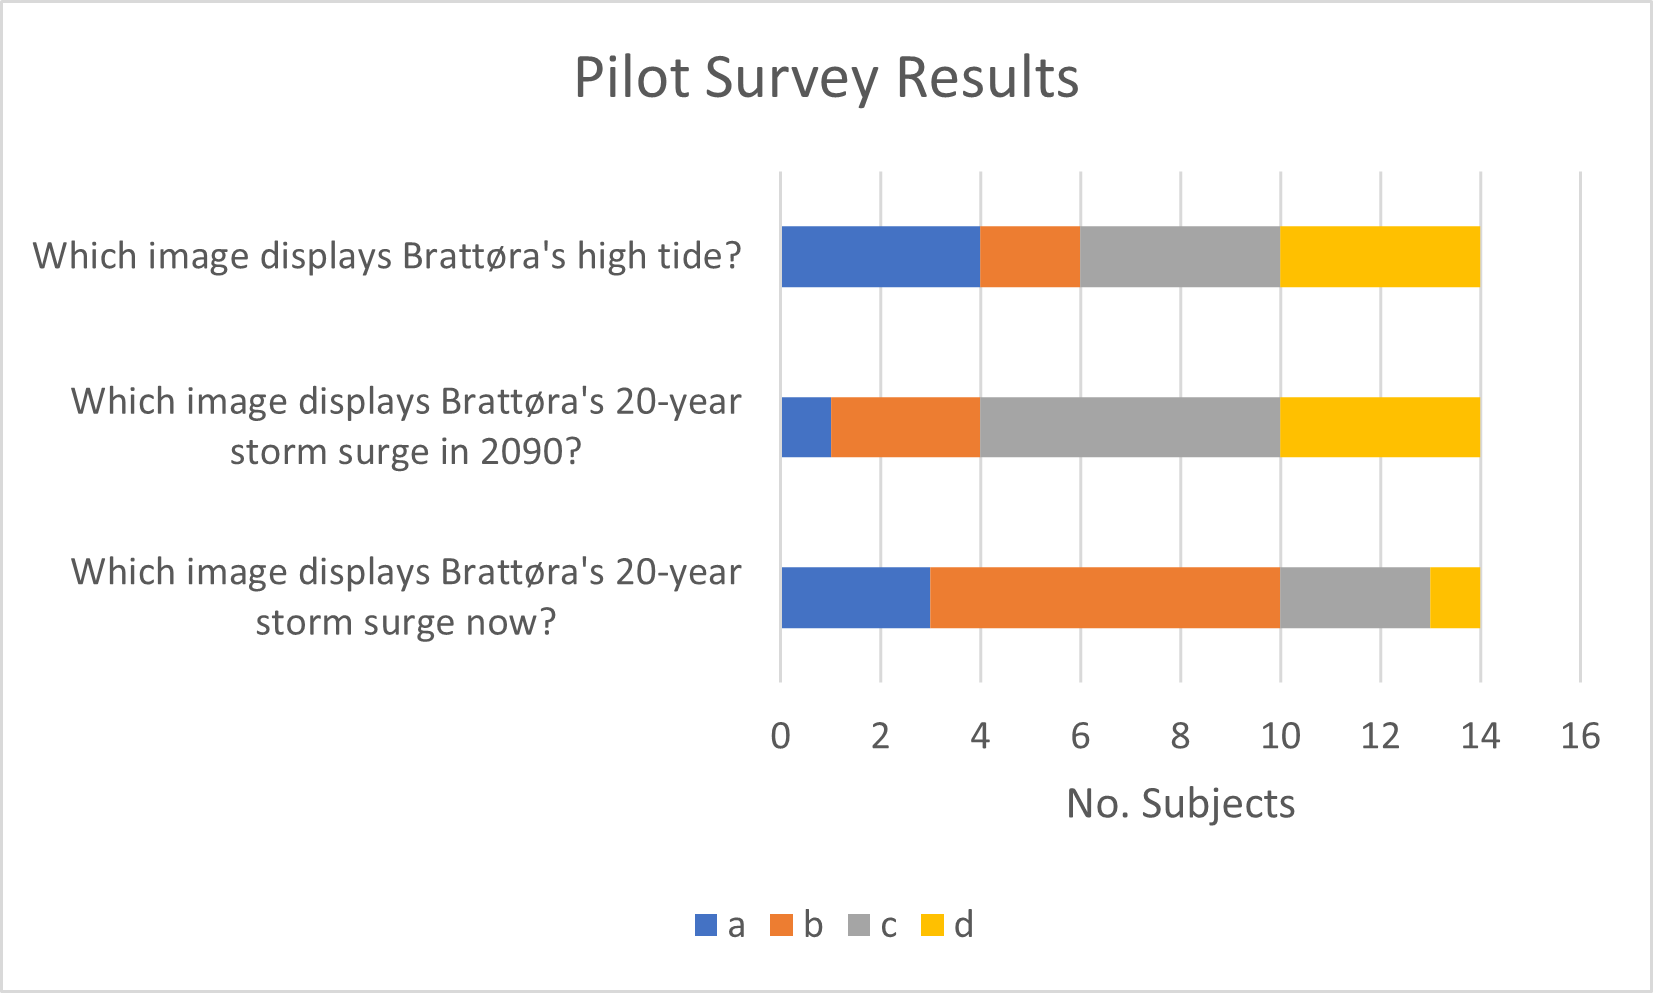
\includegraphics{fig_results/pilot_survey_results.png}
    \caption{Staked Bar Chart of Pilot Survey Results - 14 subjects asked three questions about SLEs as displayed in the Methodology section. Answers \textbf{a,b,c,d} correspond to one of the four options for maps of different SLEs in Brattøra. Answers are colour coded: \textbf{a} is blue, \textbf{b} is orange, \textit{c} is grey and \textbf{d} is yellow. Response to the first question show no observable preference for any of the answers, the correct answer was \textbf{c}. The second questions had a preference for answer \textbf{c}, the correct answer was \textbf{b}. The third question has a preference for answer \textbf{b}, the correct answer was \textbf{b}.}
    \label{fig:pilot_survey_results}
\end{figure}

 Answers corresponding with models from (\cite{kartverket_se_2020}) are considered to be correct in this context.  For the question "Which image displays Brattøra's high tide?" the answer is C (color-coded in grey), the responses for this question were widely spread over the four options. For the question "Which image display's Brattøra's 20-year storm surge in 2090? the answer is B (color-coded in orange) and only 4/14 subjects selected that answer. For the question "Which image display's Brattøra's 20-year storm surge now?" the correct answer is B (color-coded in orange) and half of the subjects chose this answer. 
\paragraph{}


\subsection{Focus Group Feedback}
The main result from the focus group  was that the maps looked too similar, especially when using smart phones for survey completion. It was difficult to tell the maps apart due to the difficulty to identify the relatively small changes in the waterline. This was particularly the case for the question about the high tide. Furthermore, several participants highlighted that they did not think of SLEs in terms of the square metres of land which is flooded, but solely in terms of changing height. This one dimensional view (height in metres) was highlighted by the group as a limiting factor in the understanding of potential impacts. 
\paragraph{}

When the focus group were asked which type of visualisation method would be most effective and assist them in answering the questions set in the pilot survey - maps, edited photographs or numerical values (see Figure 3.4 in methodology) - the majority favoured the edited photographs, but several participants favoured the numerical visualisations.
Of those that chose numeric value visualisation, there was a recognition that was likely due to their professional background, which included utilising numeric representation of SLEs. Those with a longer knowledge of Trondheim favoured the edited photographs. This was also highlighted as the option with the highest emotional impact and the visualisation which caught the whole focus groups attention.
\paragraph{}






\section{Results from Main Survey to determine Social Systems Resilience}

This section focuses on the results obtained from the survey conducted to determine social systems resilience to SLEs in Trondheim.  It also includes the results from Kruskal Wallis Rank Sum Tests and Shapiro Tests. The outputs from the survey questions are graphically visualized and presented. These results will be discussed later to determine Trondheim's social systems resilience to SLEs. The tables and graphs in the following section make reference to the main research survey questions. The full surveys, either Norwegian or English, are available in the appendix. Reference in the text is only made to the English questions. 



\subsection{Place and language}
Table 5.1 shows the by place and language splits of the 153 subjects who completed the main survey. 
\begin{table}[H]
    \centering
    \begin{tabular}{|l|l|l|l|}
    \hline
    \textbf{Place}  & \textbf{ English} & \textbf{Norwegian} & \textbf{Total Subjects}  \\ \hline
      Skansen & 11 & 18  & 29    \\ \hline
      Nidelva & 28 & 29 & 57      \\ \hline
      Grillstad & 13 & 24 & 37       \\ \hline
      Brattøra & 14 & 16 & 30     \\ \hline
      Total & 66 & 87 & 153   \\ \hline
     \end{tabular}
    \caption{Place and language subjects chose to Answer on. The most popular sub-survey was Nidelva with 57 responses, representing 37 \% of responses. Next popular was Grillstad with 37 responses and then Brattøra with 30 and Skansen with 29 respectively. The reasonable spread of response does allow for comparison. More subjects responded in Norwegian (87) than English (66), but it was comparably split for each location whether the survey was completed in Norwegian or English. }
    \label{tab:place_language}
\end{table}
\paragraph{}

The most popular place for responses was Nidelva, followed by Grillstad, Brattøra and finally Skansen. Almost evenly split for each location was whether the survey was completed in Norwegian or English. Overall responses in English totalled 66, while the Norwegian survey had 87 responses.  

\subsection{Interest Level in SLEs}
The following two figures (Figure 5.3 and Figure 5.3) show the results from the survey questions on self-ranking interest level. 80 \% of subjects responded with a medium or higher level of interest. 


\begin{figure}[H]
    \centering
    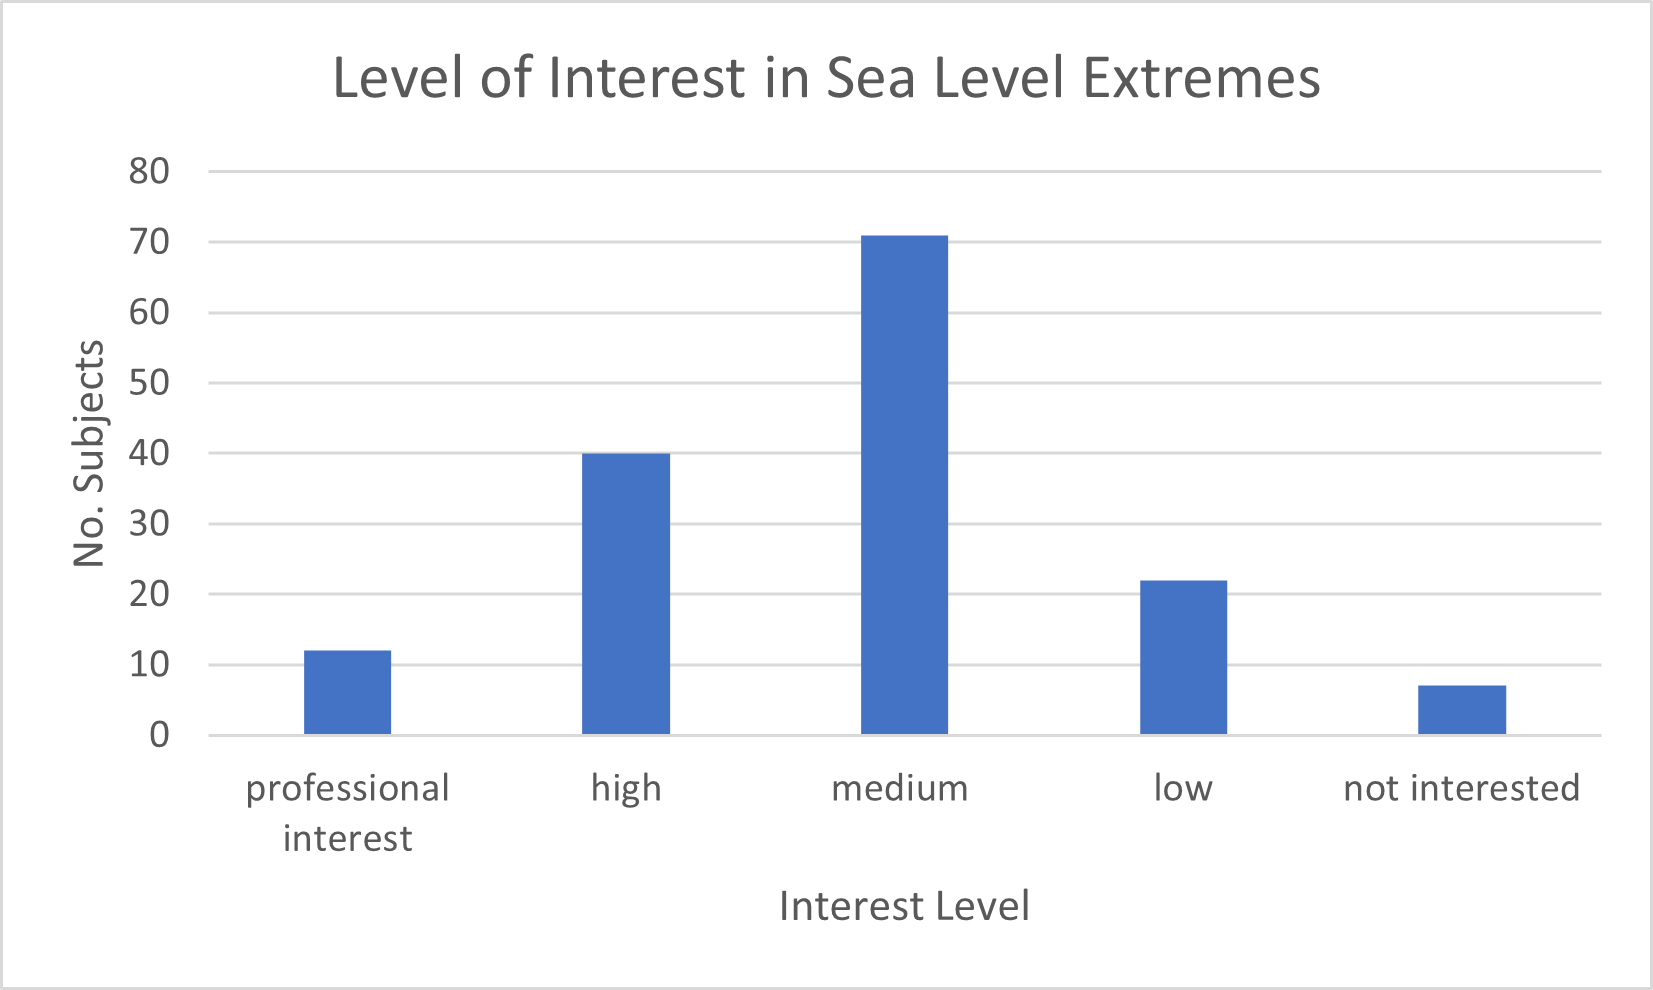
\includegraphics{fig_results/interest-level.png}
    \caption{Interest Level in SLEs - There is a good spread in the results to this question. 22 subjects have low interest in SLEs, 7 are not interested.  Almost half of the subjects (71/153) answered that they have a medium interest in SLEs. More subjects answered that they had a high level of interest (40) than have a low level of interest in SLEs. 12 subjects answered that they have professional interest in SLEs. }
    \label{fig:interest_level_SLE}
\end{figure}
\paragraph{}

The majority of respondents answered that their interest in SLEs is medium. Interestingly, 7 subjects responded that they have no interest, while 12 subjects responded that they have a professional interest in SLEs. 
\paragraph{}
Figure 5.11 displays awareness against self-ranking interest level.

\begin{figure}[H]
    \centering
    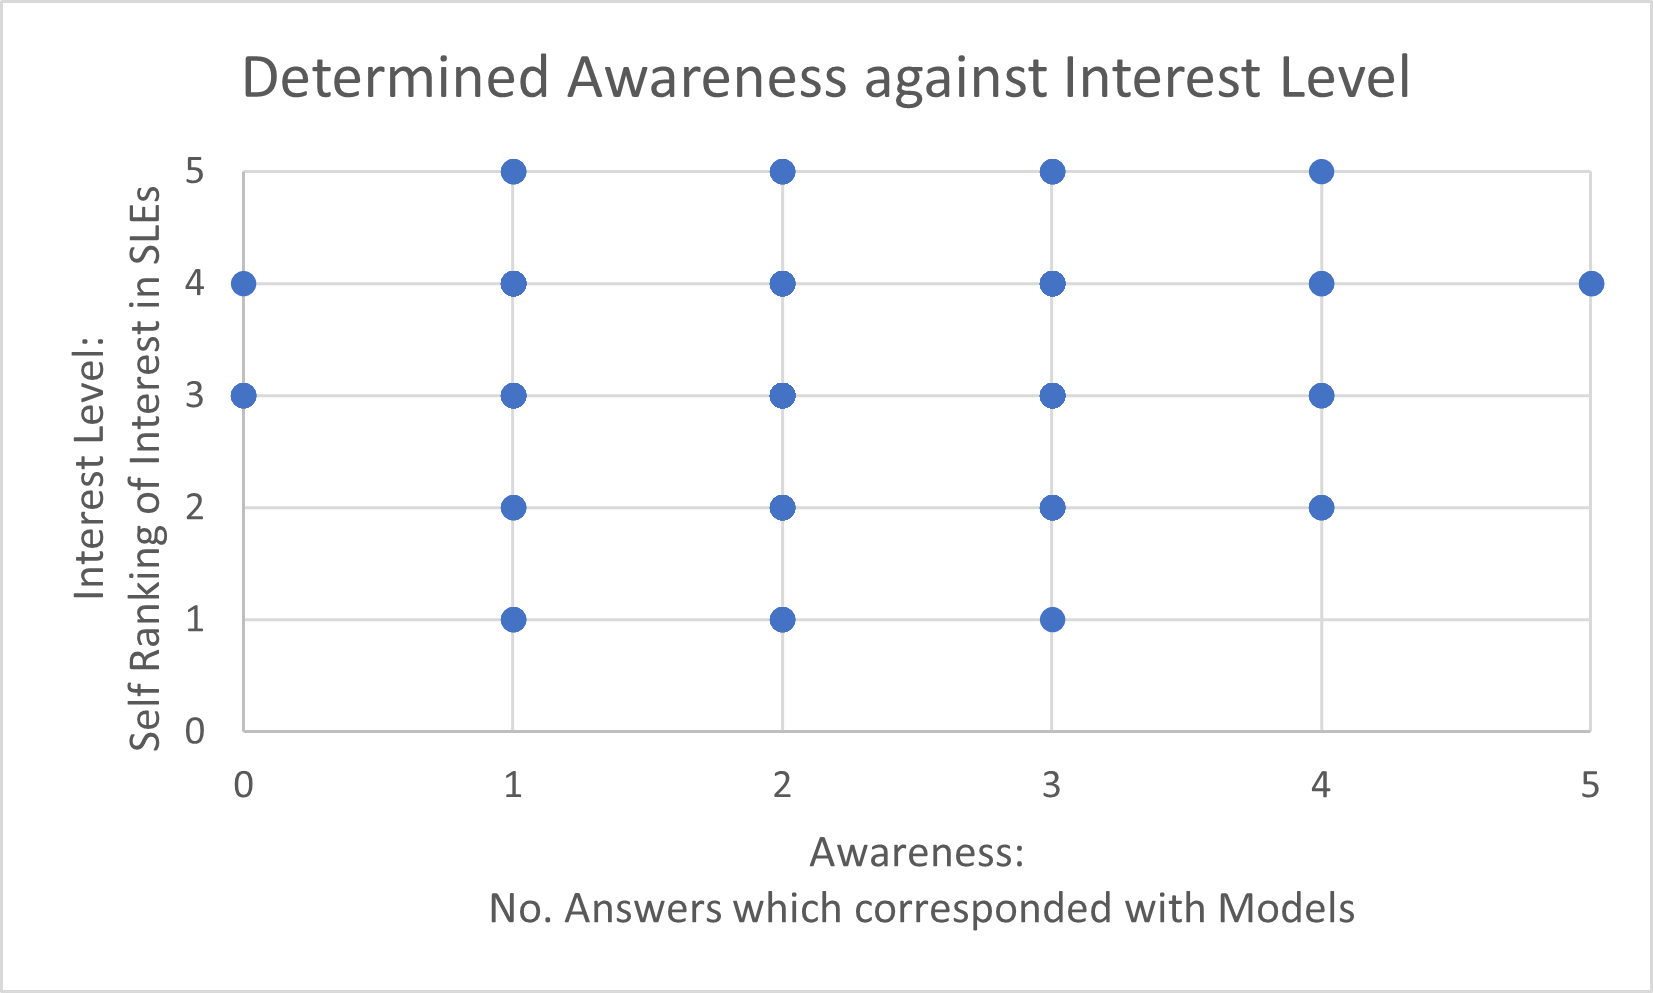
\includegraphics{fig_results/aware_vs_interest.png}
    \caption{Determined Awareness Against Interest Level -  Professional interest is level 5 on the y-axis, High  is level 4, medium is level 3, 2 is low interest and 1 is not interested. Subjects who responded high levels of interest are determined as representing all levels of awareness.}
    \label{fig:aware_vs_interest}
\end{figure}
\paragraph{}

There is no linearity or other pattern observed in Figure 5.11. Medium level self ranking of interest has almost as broad a variation as high level, but does not include any subjects who were determined to have the highest level of awareness.  It is worth noting  that Figure 5.11 does not display how often subjects interest level matched their awareness. A single subject is enough for a blue dot to be displayed as there is no weighting with this Figure, though this can be inferred from figure 5.10. 


\subsection{Memory of SLEs and Length of Place-based Knowledge}
The spread of the memory of sea level extreme events in Trondheim by the subjects is shown in figure 5.12.

\begin{figure}[H]
    \centering
    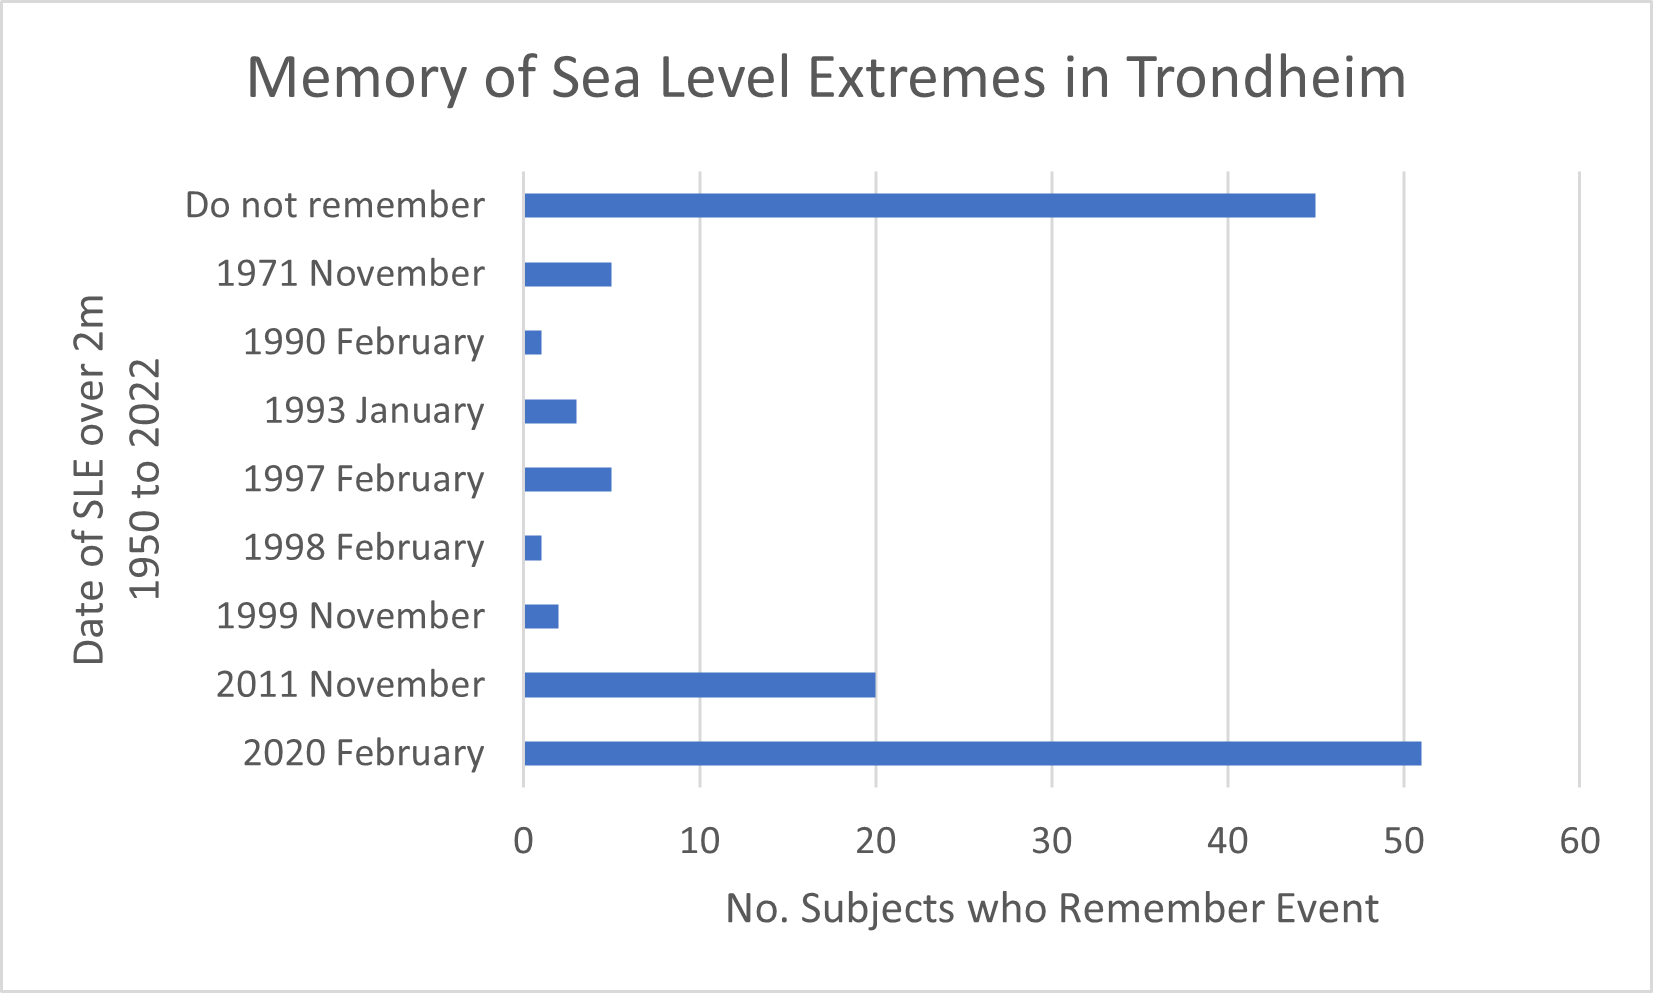
\includegraphics{fig_results/memory-sle.png}
    \caption{Memory of SLEs - The subjects were asked which about each sea level extreme event (water level higher than 2m) they remembered occurring between 1950 and summer 2022. For the full list of potential events please consults the relevant question in the appendix. 45 out of 153 subjects do not remember any sea level extreme event in Trondheim. Only one subject remembered every sea level extreme event dating back to 1950 in Trondheim. 51 subjects remembered the sea level extreme event in February 2020. }
    \label{fig:memory_sle}
\end{figure}
\paragraph{}

Memory has a very skewed factor. 30\% of subjects have no memory of SLEs in Trondheim. Once that answer is excluded, there is almost an exponential increase in the number of subjects who remember the event the closer to the present. 
\paragraph{}
Figure 5.13 shows the responses to the place-based length of knowledge question.

\begin{figure}[H]
    \centering
    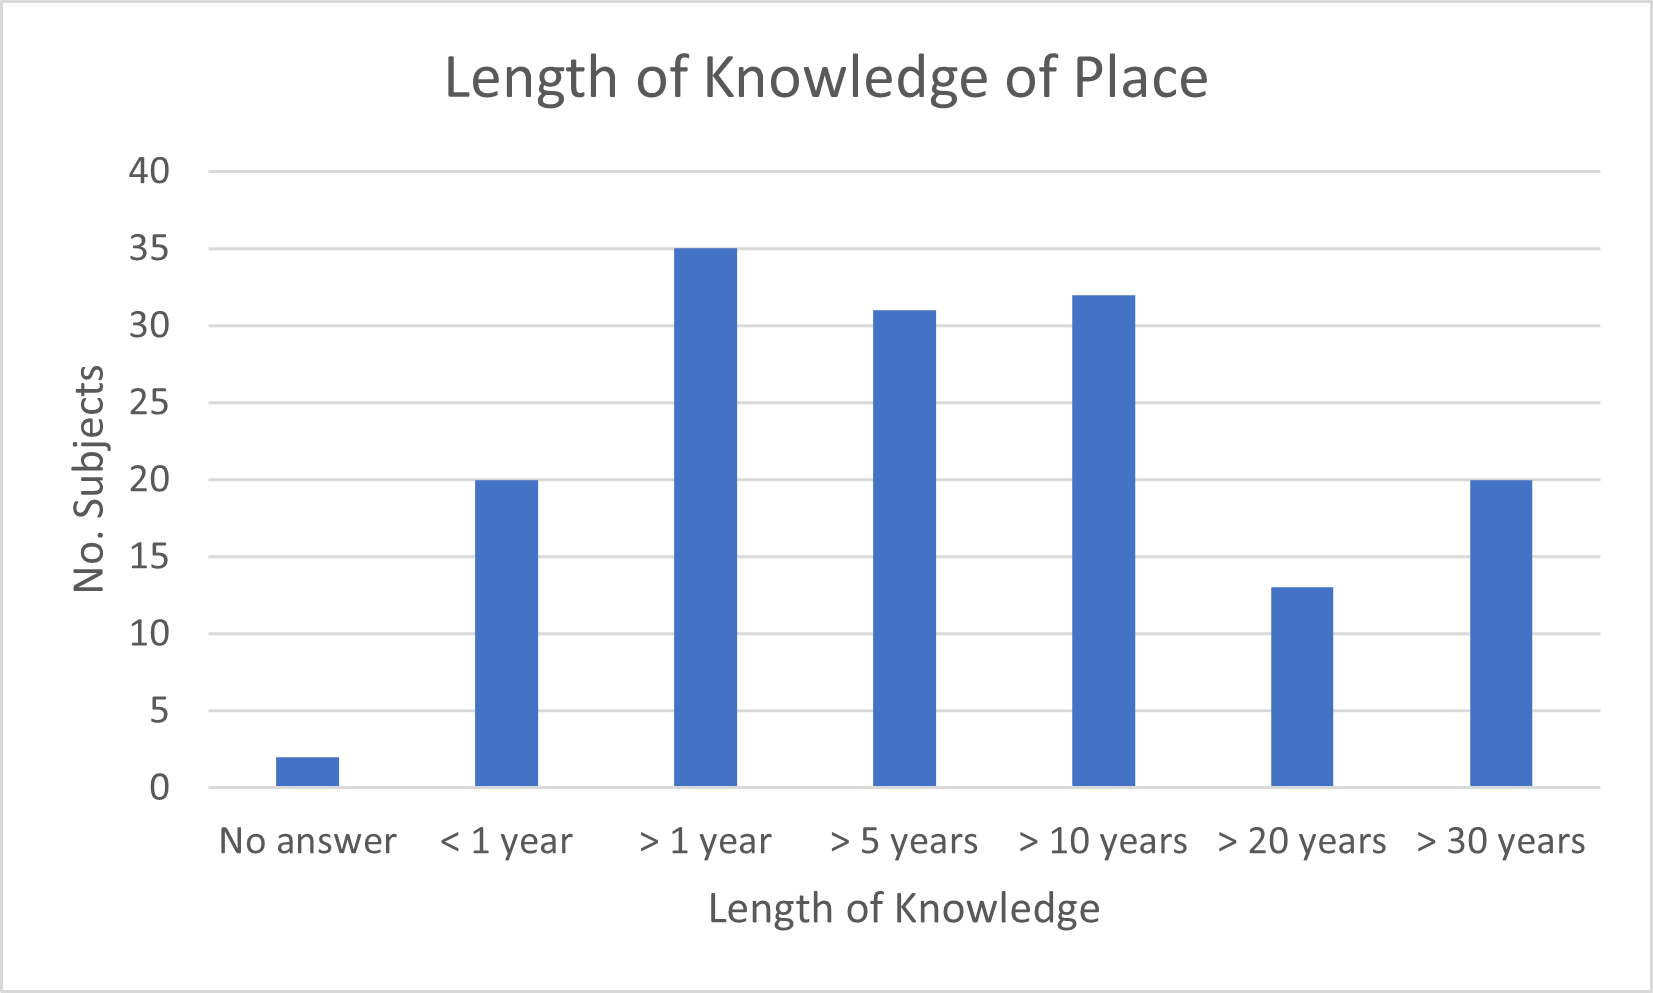
\includegraphics{fig_results/long_know.png}
    \caption{Length of Knowledge of Subjects. 96 subjects had a length of knowledge about the place greater than 5 years 35 subjects had length of knowledge less than 5 years, but more than 1. Only 20 respondents had a length of knowledge under 1 year}
    \label{fig:long_know}
\end{figure}

20 subjects responded that they had a length of knowledge of Trondheim under one year. 96 subjects responded that they had a length of knowledge greater than five years, which includes the sea level extreme event occurring in February 2020, which only 51 subjects remembered. The difference between a sea level extreme event and a disaster and how this impacts memory and resilience is expanded upon in the discussion.


\subsection{Information Access about Climate and Place}
There is significant skew in how subjects access information about climate and place as can be seen in Table 5.3 and Table 5.4 below. That individuals with a broader range of information sources have higher levels of awareness is one of the hypotheses outlined in the introduction. 

\begin{center}
\begin{table}[H]
    \centering
    \begin{tabular}{|l|l|l|l|l|l|l|}
    \hline
        \textbf{Factor} & \textbf{mean} & \textbf{Std Dev}. & \textbf{ min} & \textbf{max} & \textbf{ range} & \textbf{skew}  \\ \hline
        
      Sum of Information Access & 3.50 & 1.72 & 0 & 8 & 8 & 0.24 \\ \hline
        Personal Observation  & 0.45 & 0.50 & 0 & 1 & 1 & 0.20 \\ \hline
        Family & 0.18 & 0.38 & 0 & 1 & 1 & 1.68  \\ \hline
        Friends & 0.23 & 0.42 & 0 & 1 & 1 & 1.28  \\ \hline
        Newspapers & 0.72 & 0.45 & 0 & 1 & 1 & -0.96 \\ \hline
        TV & 0.46 & 0.50 & 0 & 1 & 1 & 0.14 \\ \hline
        Social Media & 0.63 & 0.48 & 0 & 1 & 1 & -0.55 \\ \hline
        Membership of Organisations & 0.14 & 0.35 & 0 & 1 & 1 & 2.09 \\ \hline
       Peer Reviewed Publications & 0.39 & 0.49 & 0 & 1 & 1 & 0.44 \\ \hline
        Formal Education & 0.29 & 0.46 & 0 & 1 & 1 & 0.89 \\ \hline
        
         \end{tabular}
    \caption{Information about Climate Summary Statistics information access}
\label{table:summary_stats_info_access}
\end{table}
\end{center}

\begin{center}
\begin{table}[H]
    \centering
    \begin{tabular}{|l|l|l|l|l|l|l|}
    \hline
         \textbf{Factor} & \textbf{mean} & \textbf{Std Dev.} & \textbf{min} & \textbf{max} & \textbf{range} & \textbf{skew}  \\ \hline
        Sum of Information Access & 1.94 & 1.34 & 0 & 8 & 8 & 1.61 \\ \hline
        Personal Observation & 0.73 & 0.45 & 0 & 1 & 1 & -1.00  \\ \hline
        Family & 0.10 & 0.31 & 0 & 1 & 1 & 2.56 \\ \hline
        Friend & 0.19 & 0.39 & 0 & 1 & 1 & 1.57  \\ \hline
        Newspaper & 0.35 & 0.48 & 0 & 1 & 1 & 0.64  \\ \hline
        TV & 0.14 & 0.35 & 0 & 1 & 1 & 2.09 \\ \hline
       Social Media & 0.33 & 0.47 & 0 & 1 & 1 & 0.73  \\ \hline
        Membership of Organisations & 0.04 & 0.19 & 0 & 1 & 1 & 4.70 \\ \hline
        Trondheim Municipality & 0.07 & 0.26 & 0 & 1 & 1 & 3.28\\ \hline
                
         \end{tabular}
    \caption{Information about Place Summary Statistics information access}
\label{table:summary_stats_info_access}
\end{table}
\end{center}

Social media is a more common response for information about climate than information about place. Membership of organisations is the least popular response for both information about climate and place. Personal observation is the most popular response for information about place and the fourth most popular response for information about climate. On average, subjects selected more sources for information about climate than information about place. 
\paragraph{}
These highly skewed responses with a large variation in mean and standard deviation impacted the type of hypothesis testing which could be carried out.  

\subsection{Community Membership}
Subjects were self-selecting stakeholders.  As stated in the methods, they were asked to identify themselves as members of communities that were highlighted by a stakeholder analysis. They were also given the choice to write in other community membership if they selected other. Figure 5.14 displays the community memberships selected by the subjects. 

\begin{figure}[H]
    \centering
    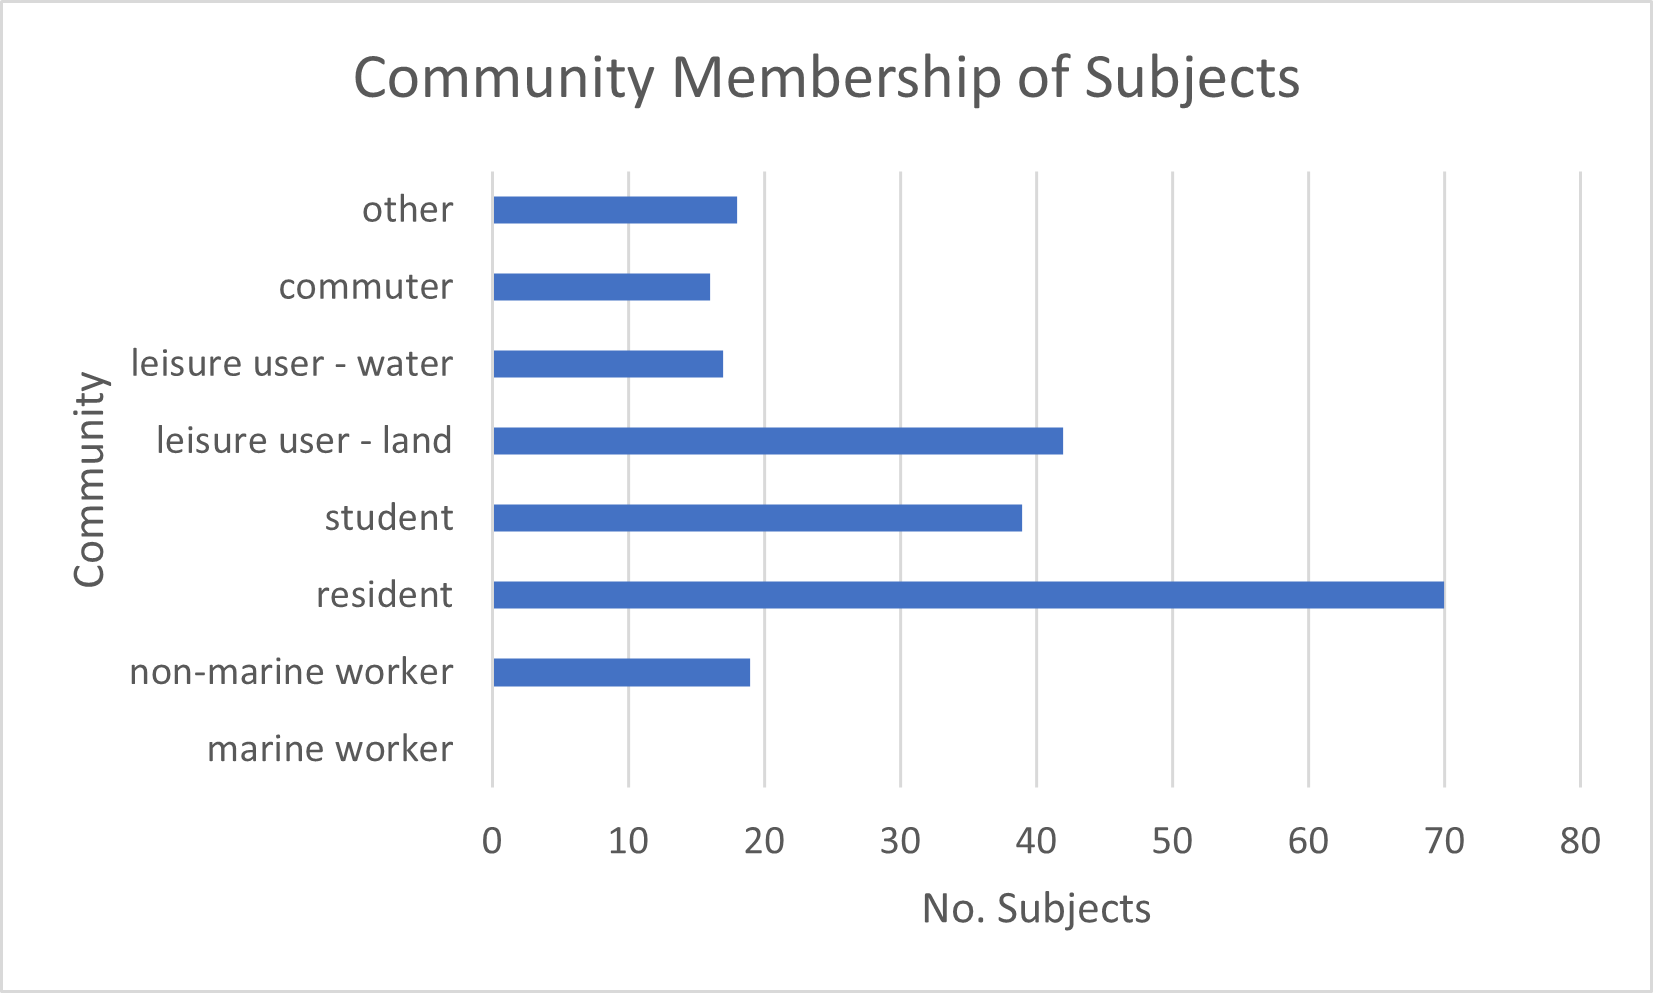
\includegraphics{fig_results/com-mem-horizontal.png}
    \caption{Membership of Communities. There were 221 selections done by the 153 subjects. However many subjects only selected one community. The most selected community was resident, however only 70 out of 153 subjects - under half. }
    \label{fig:community_membership}
\end{figure}
\paragraph{}

There are 70 subjects who answered that they are residents. This is the most common choice. Very few subjects who answered they were students also selected a second community membership. Subjects who answered as other were either visitors, tourists or sailors. That subjects only ticked one box in the survey means it is unlikely that they responded with every community that they are part of, just the identity they feel is most important. No subjects responded as marine workers. The impact of subjects only selecting a single response in this format of question is discussed in the discussion of framework. 


\subsection{Access to Survey. }
Figure 5.15 shows how subjects accessed the survey.  

\begin{figure}[H]
    \centering
    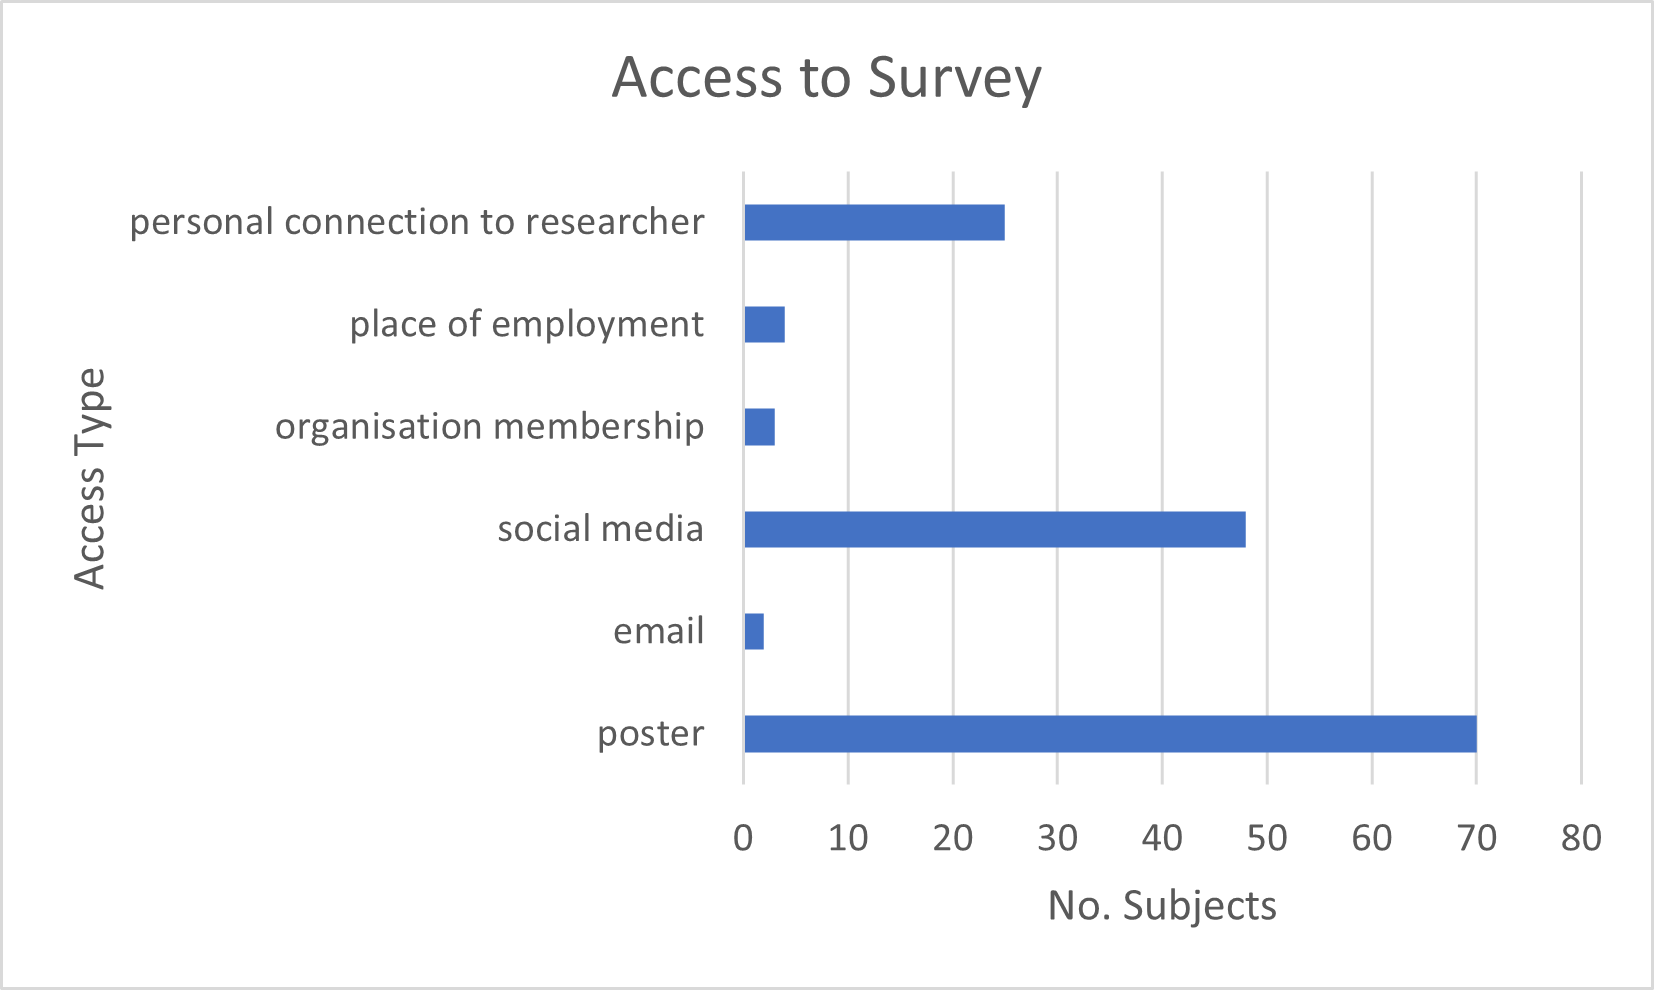
\includegraphics{fig_results/access_survey.png}
    \caption{Access to Survey - Six access types were included and the number of subjects who chose each is shown. }
    \label{fig:survey_access}
\end{figure}
\paragraph{}


The most common access method of the survey was poster, with 70 subjects selecting this choice. This is followed by social media which has 47 subjects choosing this. 25 subjects accessed the survey due to personal connection to researcher. Accesses via email, place of employment and organisation membership are all under 10. Subjects could chose more than one access type. For example, a subject could have accessed via personal connection to researcher and social media, due to the researcher sharing this survey on their personal social media.  
\paragraph{}



\subsection{Perceived Risks}
Figure 5.16 shows the  number of responses selecting a perceived risk to infrastructure. Figure 5.17 shows the number of responses selecting a perceived risk to people. .

\begin{figure}[H]
    \centering
    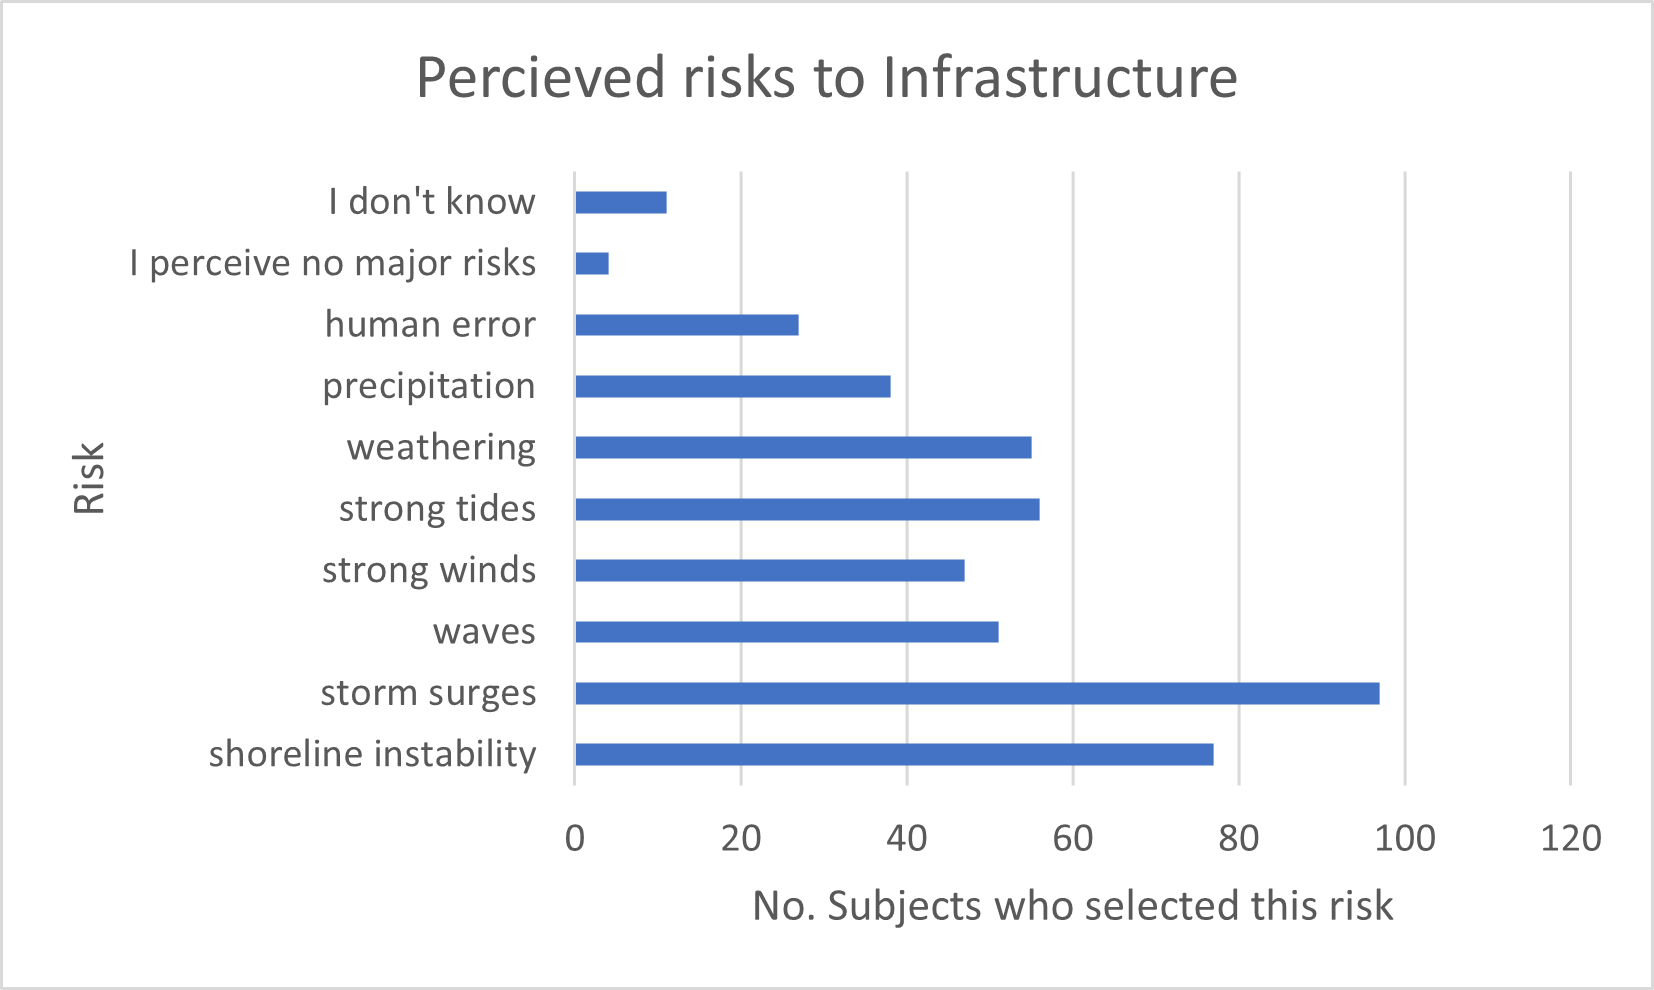
\includegraphics{fig_results/percieved risks to infrastructure.png}
    \caption{Perceived risks to Infrastructure Risks - 97 subjects selected storm surges as a risk to infrastructure. Only 4 subjects responded that they perceived no major risks to infrastructure and 11 subjects responded that they don't know. Human error was only selected by 27 subjects making it the risk the least number of subjects were concerned about. There is greater perception of weather impacts on infrastructure with 47 subjects highlighting strong winds, 51 subjects selecting waves, 56 subjects selecting strong tides and 38 selecting precipitation. After storm surges which were mentioned multiple times in the survey there is a perception of shoreline instability with 77 subjects selecting it as a risk to infrastructures.   }
    \label{fig:risk_infrastructure}
\end{figure}
\paragraph{}





\begin{figure}[H]
    \centering
    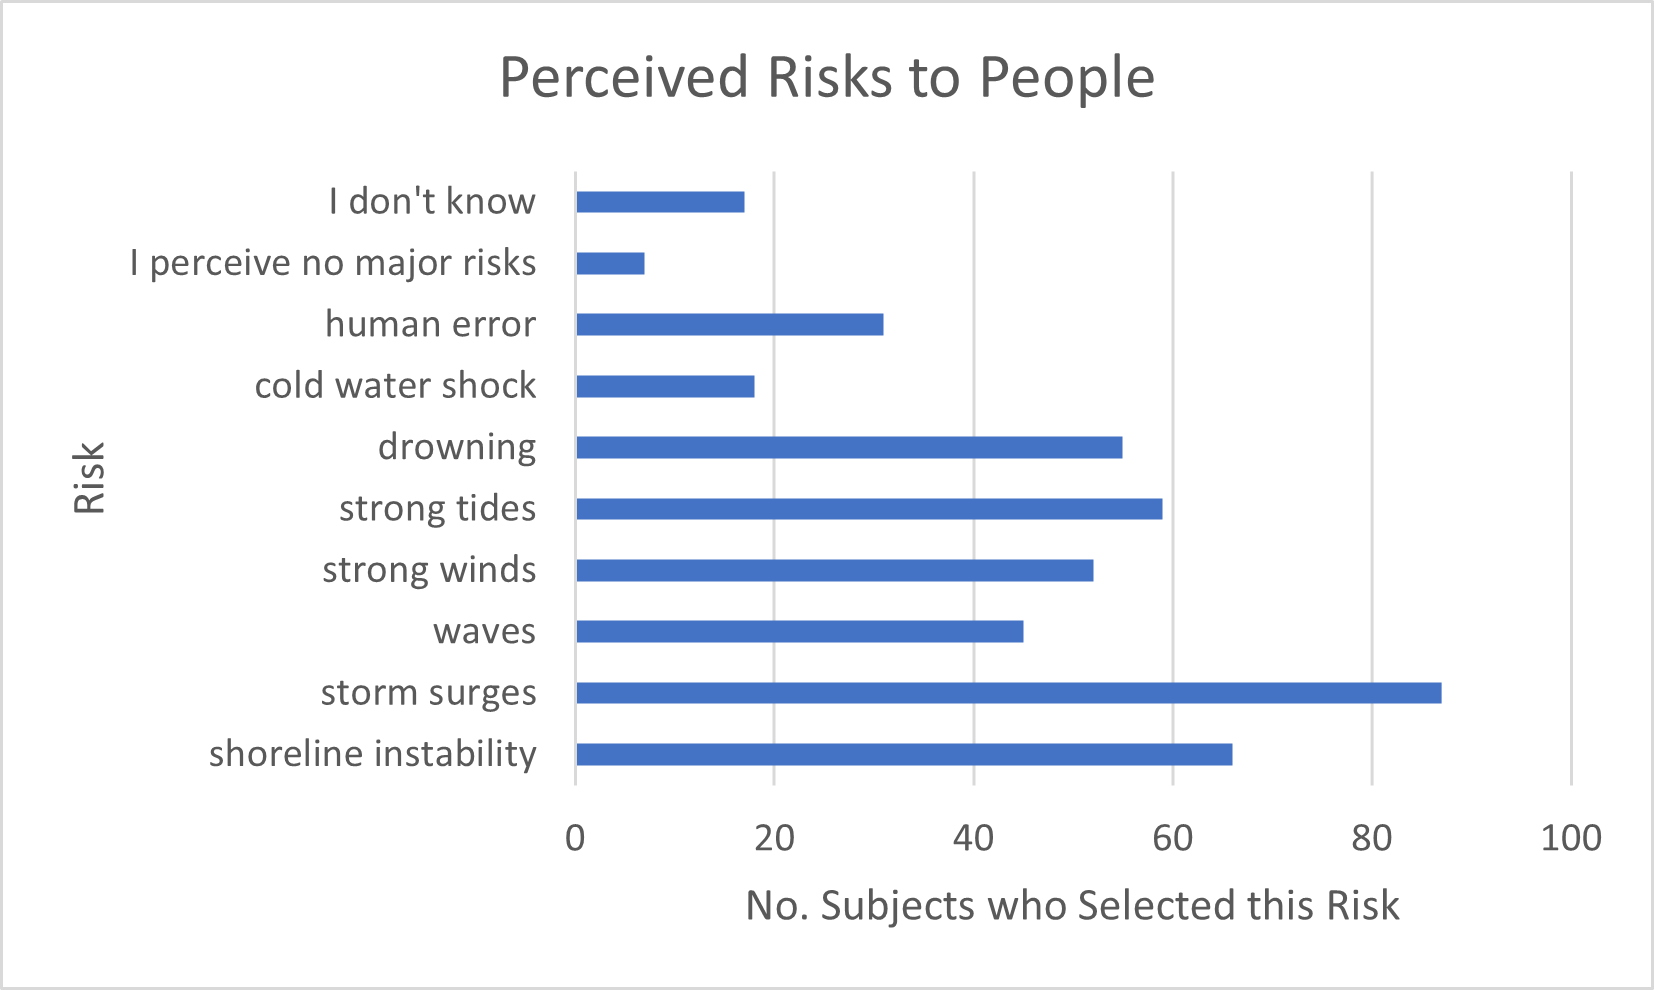
\includegraphics{fig_results/percieved risks to people.png}
    \caption{Perceived risks to People. 66 subjects selected that they perceive storm surges as a risk to people in the research sites. }
    \label{fig:risk_people}
\end{figure}
\paragraph{}
It is interesting that more than 80 subjects have selected storm surges as a risk to infrastructure or people. Shoreline instability is also a very common response across both questions. It is notable that the vast majority of subjects do identify risks to people and infrastructure for these places when offered answers. The response of "I don't know" is more common that the "I perceive no major risks". 


\section{Determination of Subjects' Awareness}
Figure 5.18 shows that the subjects displayed a high awareness of the tides in Trondheim. 

\begin{figure}[H]
    \centering
    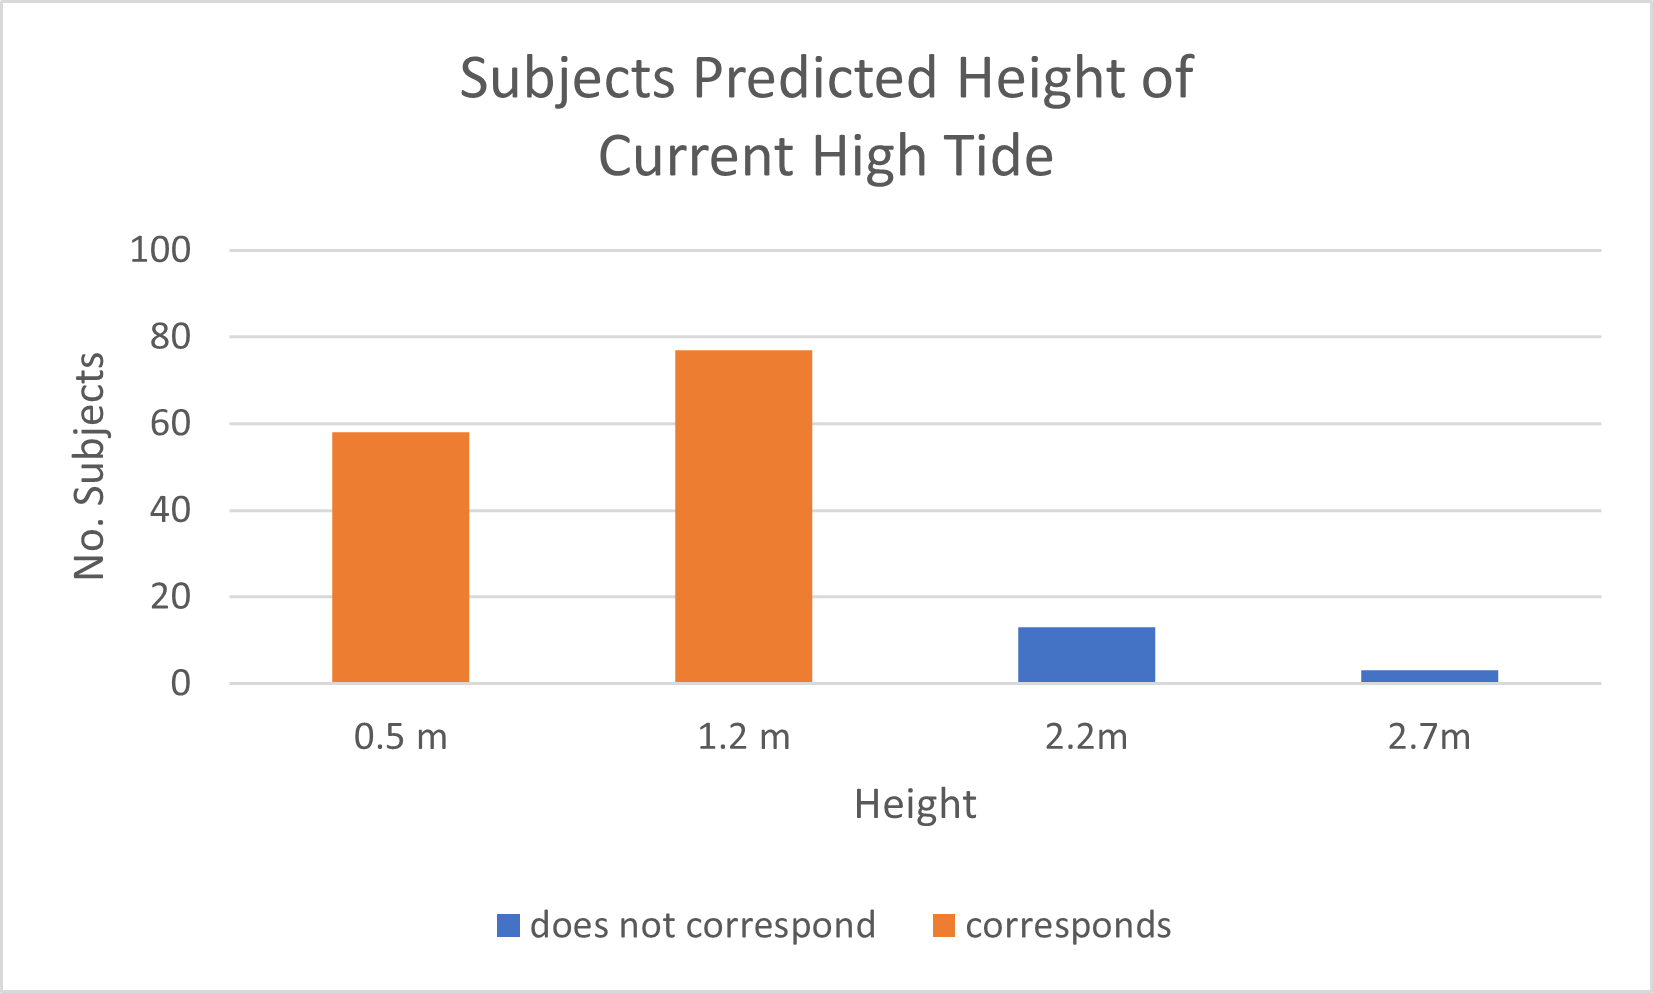
\includegraphics{fig_results/2022-hightide-answers.png}
    \caption{Subjects Predicted Height of Current High Tide. Height 0.5m is the neap high tide, Height 1.2m is the Spring High Tide. The vast majority of subjects selected a value which corresponds with models of tides in Trondheim. Under 20 subjects responded with a value which does not correspond with models of tides. 58 subjects chose 0.5m, 77 subjects chose 1.2m meaning that 135 out of 153 subjects, 88 \% chose what could be considered the correct answer for high tide. Only 13 subjects chose 2.2m and 3 subjects chose 2.7m}
    \label{fig:high_tide_answer}
\end{figure}
\paragraph{}

The height chosen largely corresponds with either the spring or neap high tide - over 80 \% of subjects chose a value which corresponds with the models from (\cite{kartverket_se_2020}). Under 20 subjects responded with a value which does not reflect the models from (\cite{kartverket_se_2021}). 
\paragraph{}
Figure 5.19 shows the responses to the question on the predicted height of the current 20 year storm surge. 
\begin{figure}[H]
    \centering
    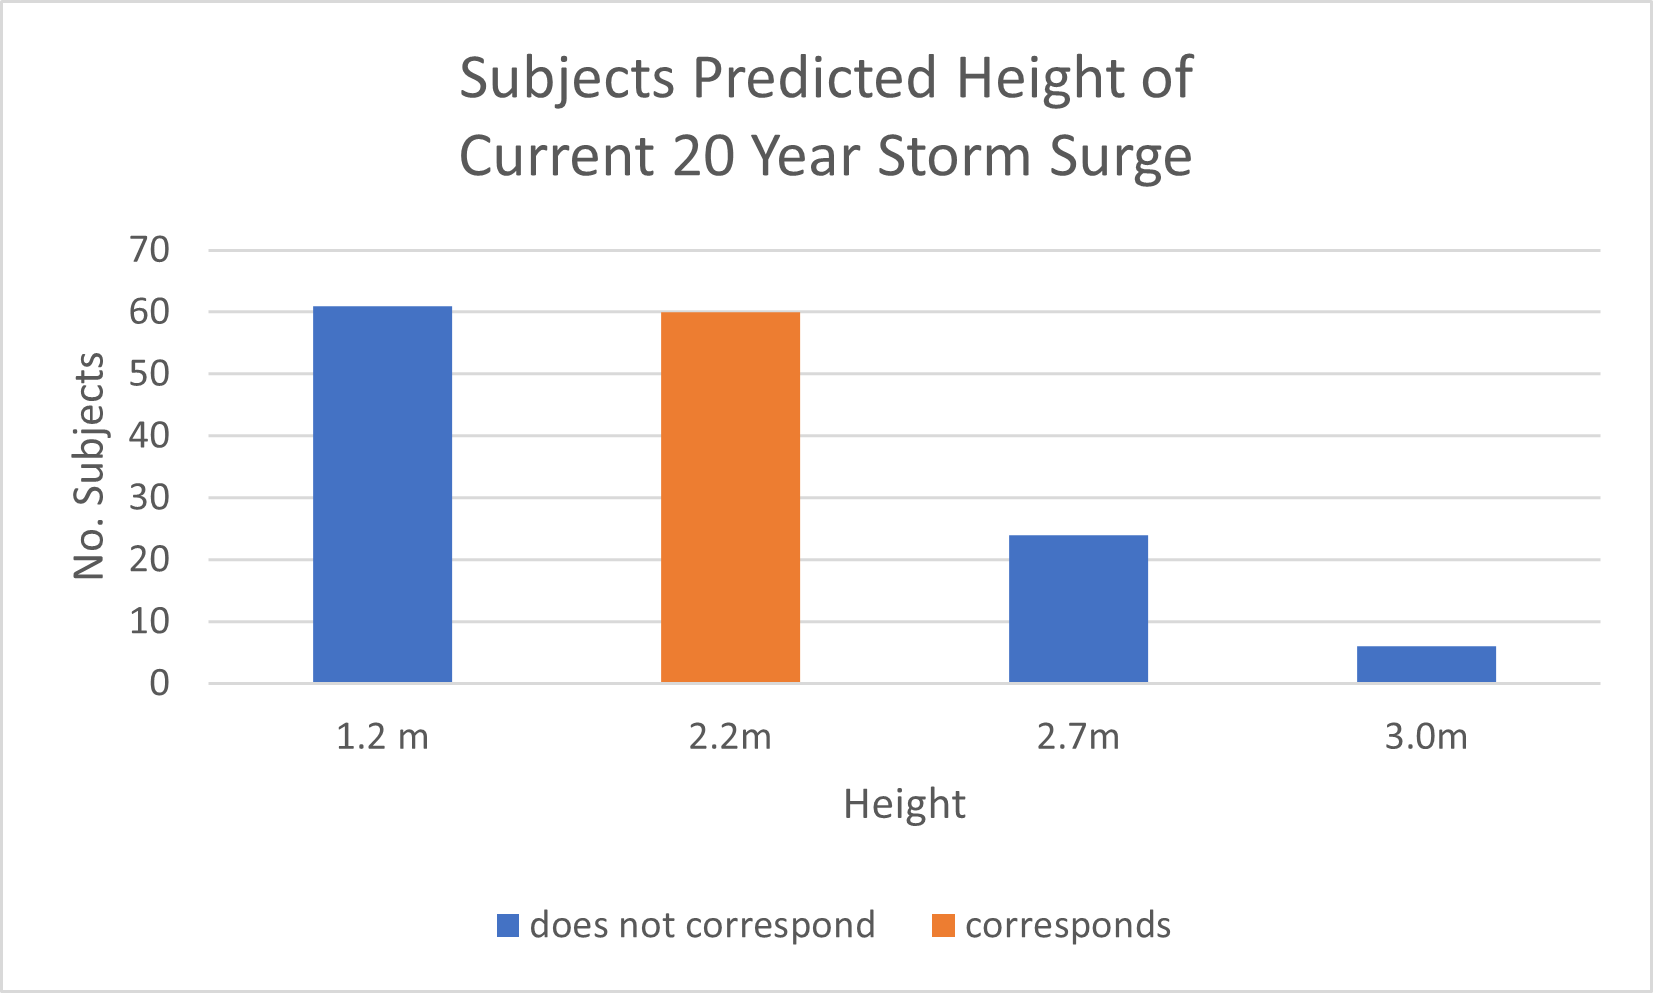
\includegraphics{fig_results/2022-20yrss-answer.png}
    \caption{Subjects Predicted Height of Current 20 Year Storm Surge. 61 subjects chose 1.2m this is very comparable to the 60 which chose 2.2m which is the answer which corresponds with (\cite{kartverket_se_2021}). 24 subjects chose 2.7m and only 6 subjects chose 3.0m}
    \label{fig:2022-stormsurge-answers}
\end{figure}
\paragraph{}
The majority of subjects chose 1.2m as the predicted height of the 20 year storm surge, but this does not correspond with models from (\cite{kartverket_se_2021}). In fact, 1.2m is equal to the current high tide. Almost equally often chosen was the answer which does correspond with models from (\cite{kartverket_se_2021}), 2.2m, with 60 subjects choosing this answer. This means that 43 \% of subjects chose the answer which corresponds with (\cite{kartverket_se_2021}). Around 20 \% (30/153) of subjects chose a value higher than the models indicate.
\paragraph{}
Figure 5.20 shows the responses to the question on the predicted height of the 2090 20 year storm surge.

\begin{figure}[H]
    \centering
    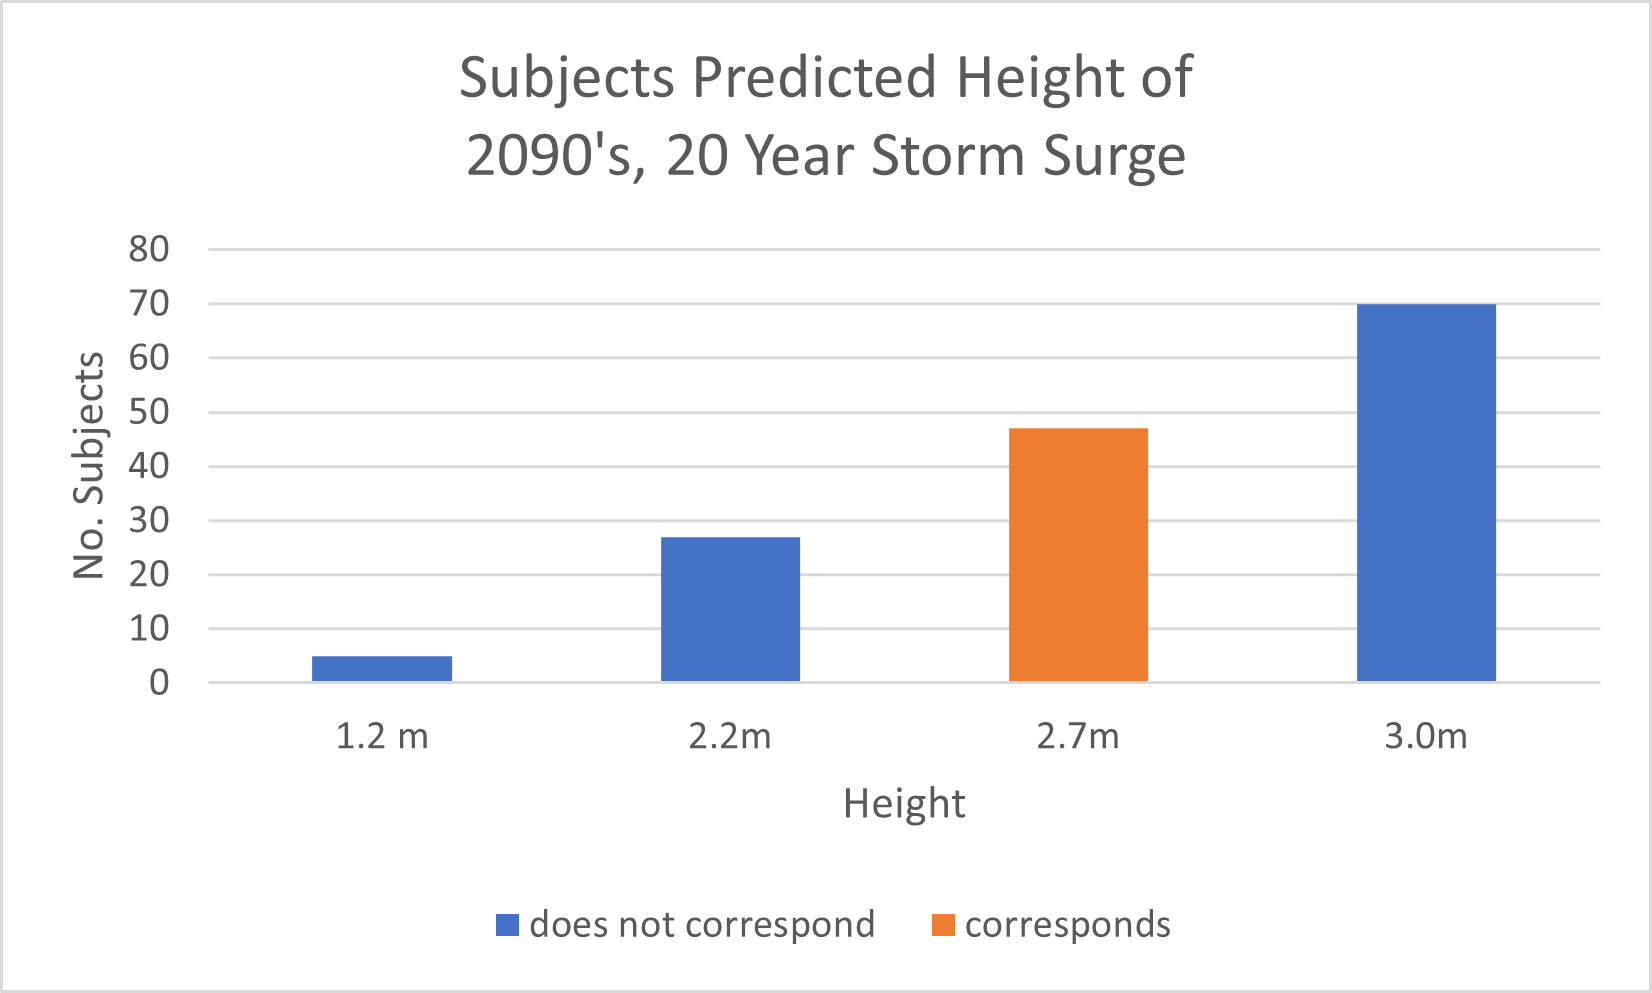
\includegraphics{fig_results/2090s 20yr ss answers.png}
    \caption{Subjects Predicted Height of 2090's, 20 year storm surge. The majority of subjects chose the highest value with 70 subjects choosing 3.0m as the predicted height of the storm surge. 47 subjects chose 2.7m which is the value which corresponds with models by (\cite{kartverket_se_2021}). 27 subjects chose 2.2m and only 5 subjects chose 1.2m}
    \label{fig:2090-stormsurge-answers}
\end{figure}
\paragraph{}
The majority of subjects predicted the storm surge in 2090 to be 3.0m. Just over 30 \% chose 2.7m which is the value which corresponds with models from (\cite{kartverket_se_2021}). This means that most people thought the sea level extreme associated with the 20 year storm surge in 2090 is higher than it is currently predicted to be. The change of height for the 20 year storm surge predicted for 2090 is only 50cm higher than the current 20 year storm surge (\cite{kartverket_se_2021}). 
\paragraph{}
Figure 5.21 shows the subjects predictions for how sea level will change in the next 30 years. 

\begin{figure}[H]
    \centering
    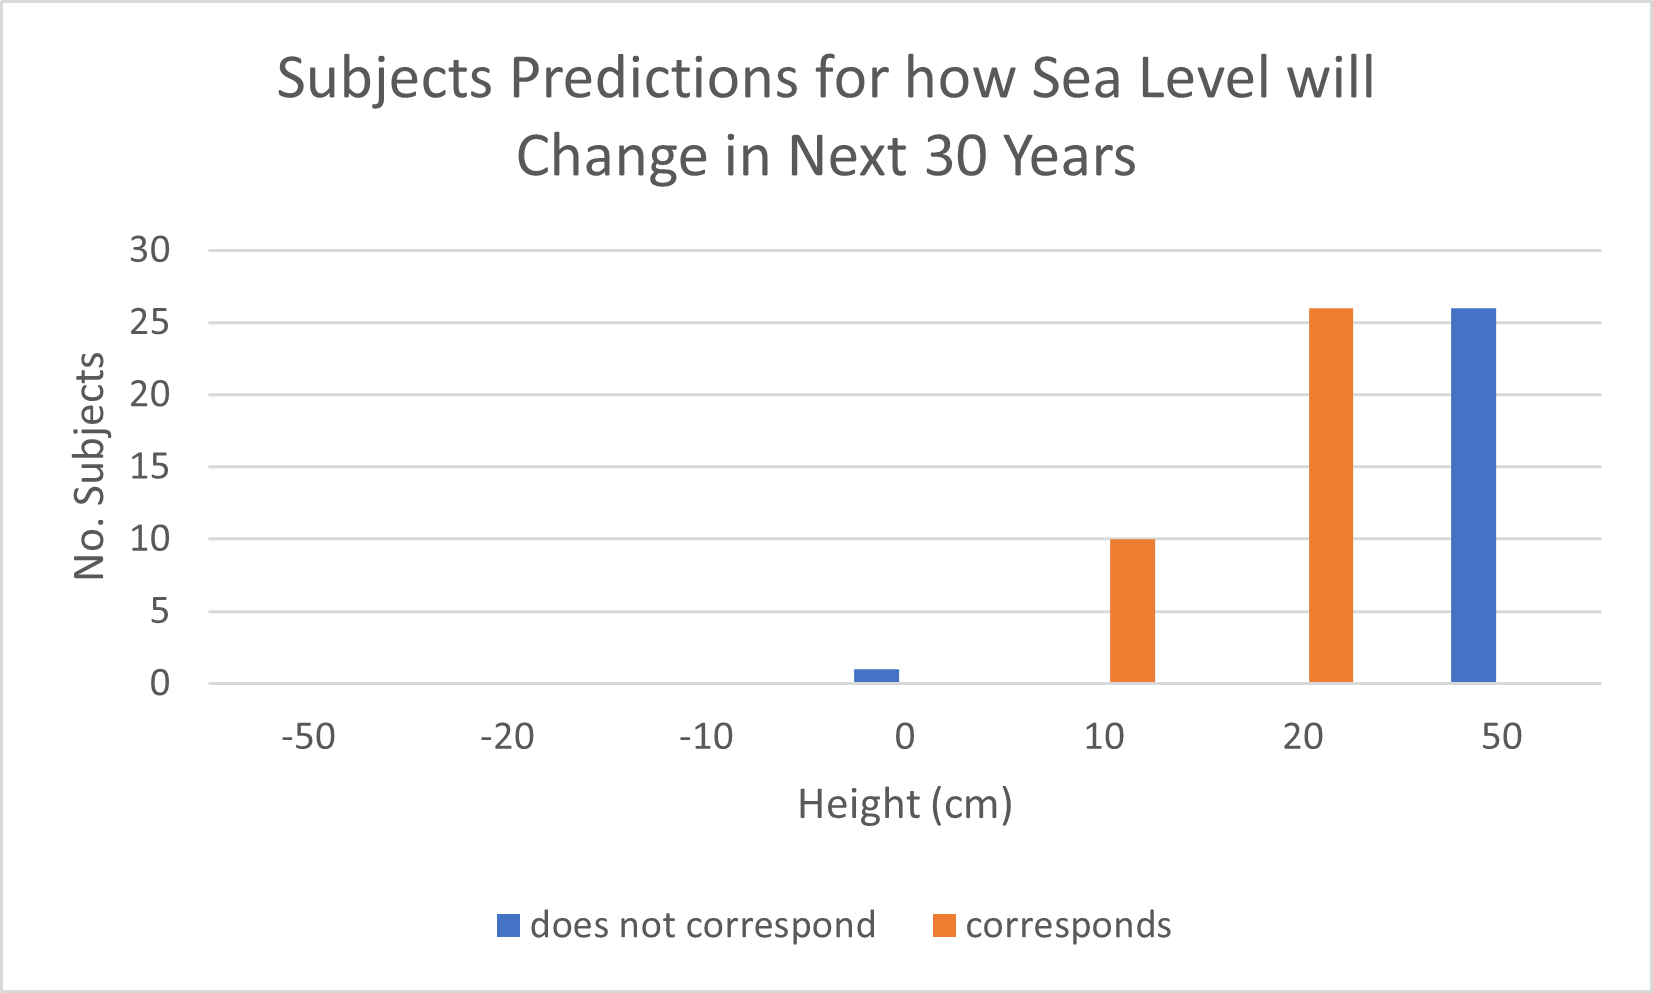
\includegraphics{fig_results/slr-future.png}
    \caption{Subjects Predictions for how Sea Level will change in Trondheim in Next 30 years. Only 147 subjects answered for this question, unlike every other one which all subjects, 153, answered. No subjects believed the sea level will decrease over the next 30 years. One subject answered that it will stay the same, with every other subject choosing that it will rise by some level }
    \label{fig:slr_future}
\end{figure}

There is strong uncertainty with this measurement in models, due to the difficulty of predicting emission patterns over the next 30 years and related glacio-isostatic uplift as they are dependent on global government policy (\cite{hanssen-bauer_climate_2017}: \cite{kartverket_se_2021}). Nevertheless, an estimation of 20cm or 10cm is in line with (\cite{kartverket_se_2021}) which uses the upper emissions pathways from the IPCC. Over half of the subjects chose a value which is in line with models from (\cite{kartverket_se_2021}). However, equal numbers of subjects, 26 , chose 50cm as chose 20cm,  which is not in line with these models. Almost all subjects answered that sea level will rise in the next 30 years, though six subjects chose not to answer this question.  

As shown in the survey attached in the appendix, Figure 5.21 and Figure 5.22 display results from questions which were purely numerical answers. There were no edited photographs to show the simulated SLEs.
\paragraph{}


\begin{figure}[H]
    \centering
    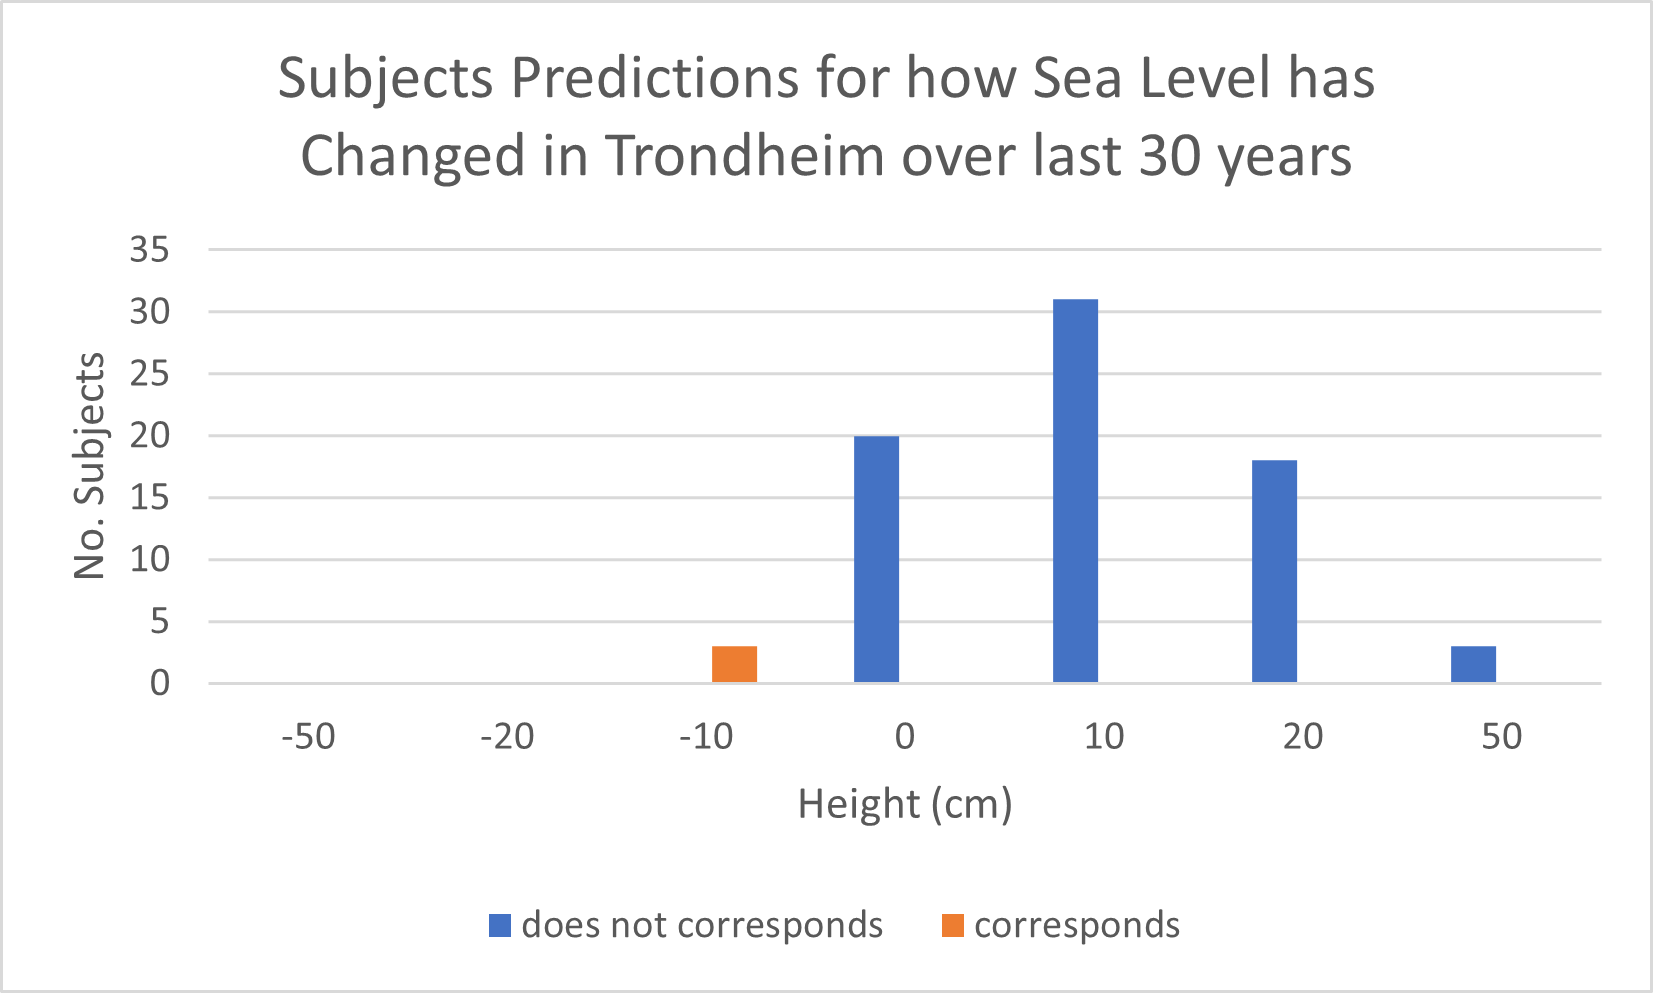
\includegraphics{fig_results/slr-past.png}
    \caption{Subjects Predictions for how Sea Level has Changed in Trondheim over last 30 years. Only 3 subjects chose that sea level has decreased in the last 30 years, this answer is inline with (\cite{kartverket_se_2021}). 20 subjects answered that sea level had not changed over this time. While 31 subjects answered that it had risen by 10 cm. 18 subjects answered that it had risen by 20 cm and 3 answered that it had risen by 50 cm. 52 subjects answered that sea level had risen over the last 30 years. }
    \label{fig:slr_past}
\end{figure}

Figure 5.22 shows the subjects predictions for how sea level has changed in Trondheim over the last 30 years. The certainty for the models presented here is high, as they are based off recordings not projections. 
\paragraph{}

Figure 5.23 is a combination of all results thus far in this section on awareness. This was the first attempt to determine awareness of subjects from the results of this survey

\begin{figure}[H]
    \centering
    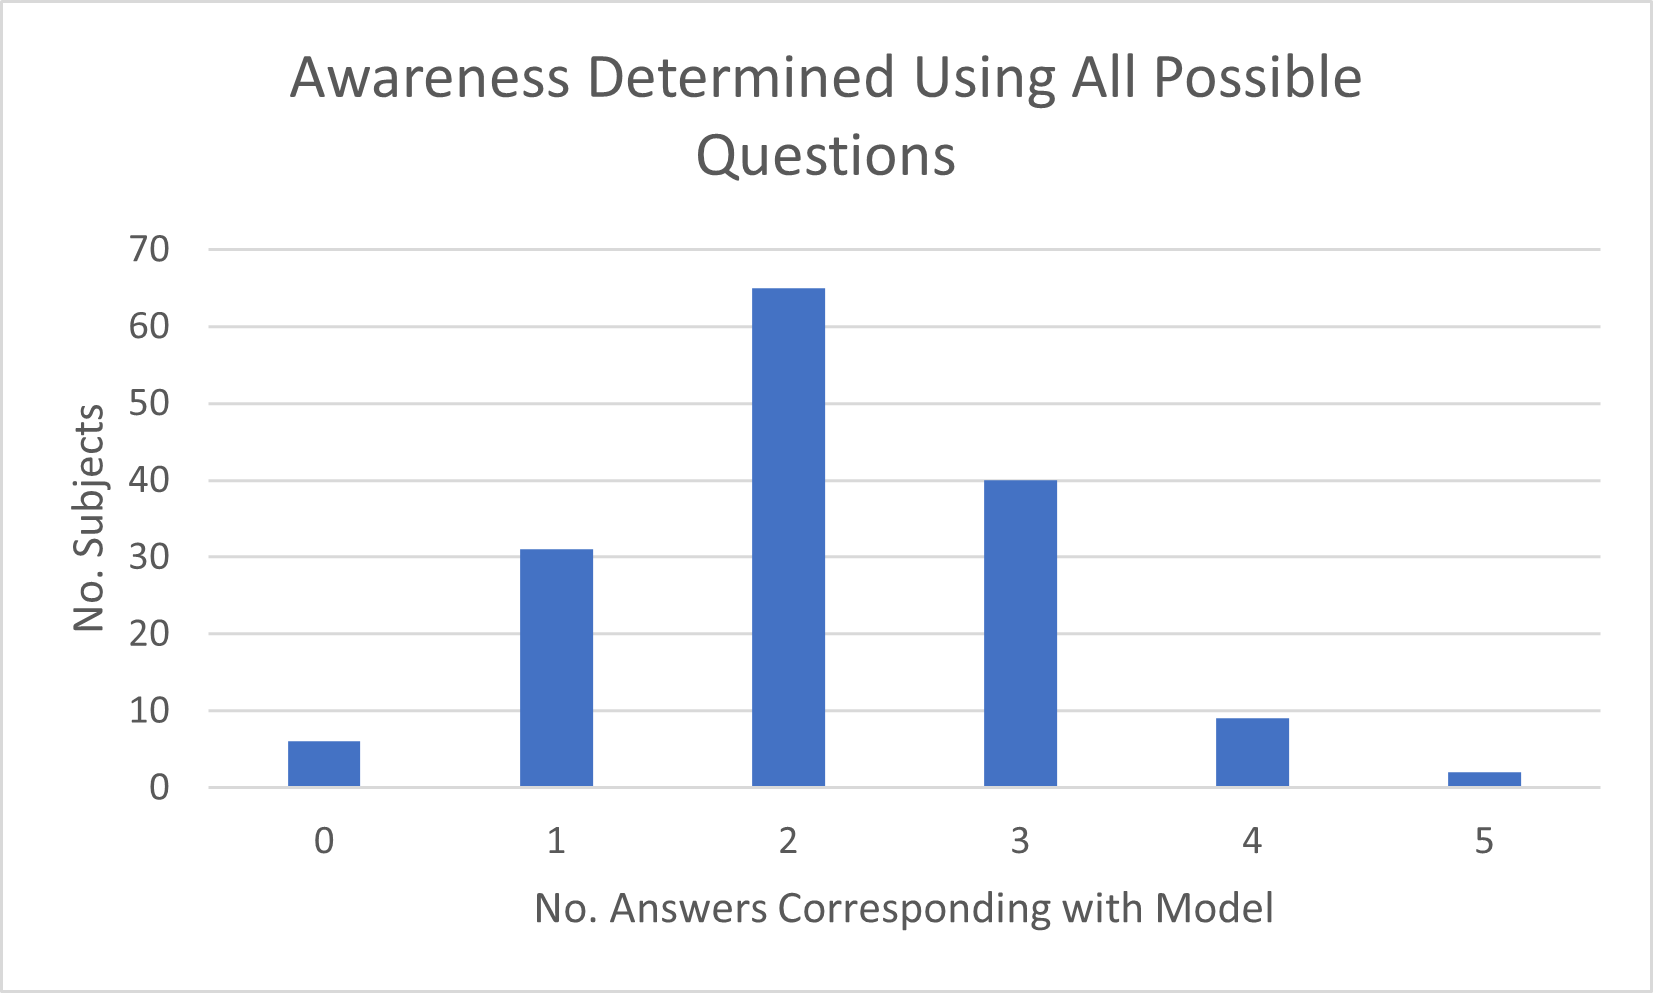
\includegraphics{fig_results/aware_all.png}
    \caption{Awareness Considering all Questions which were designed to determine awareness.  2 subjects had all answers corresponding with the models from (\cite{kartverket_se_2020}). 9 subjects had 4 answers corresponding, 40 subjects had 3 answers corresponding, 65 subjects had 2 answers corresponding, 31 subjects had 1 answer corresponding and 6 subjects had no answers corresponding. }
    \label{fig:aware_all_qs}
\end{figure}
\paragraph{}

Awareness determination considering all answers related to questions was not the most suitable for analysing factors related to awareness. For this reason, another determination of awareness was created utilising only the questions which had pictures of the simulated water levels. This is discussed further in chapter 6. 
\paragraph{}
Figure 5.24 shows determination of awareness considering the questions which utilised edited photographs, excluding the questions which were purely numeric. 

\begin{figure}[H]
    \centering
    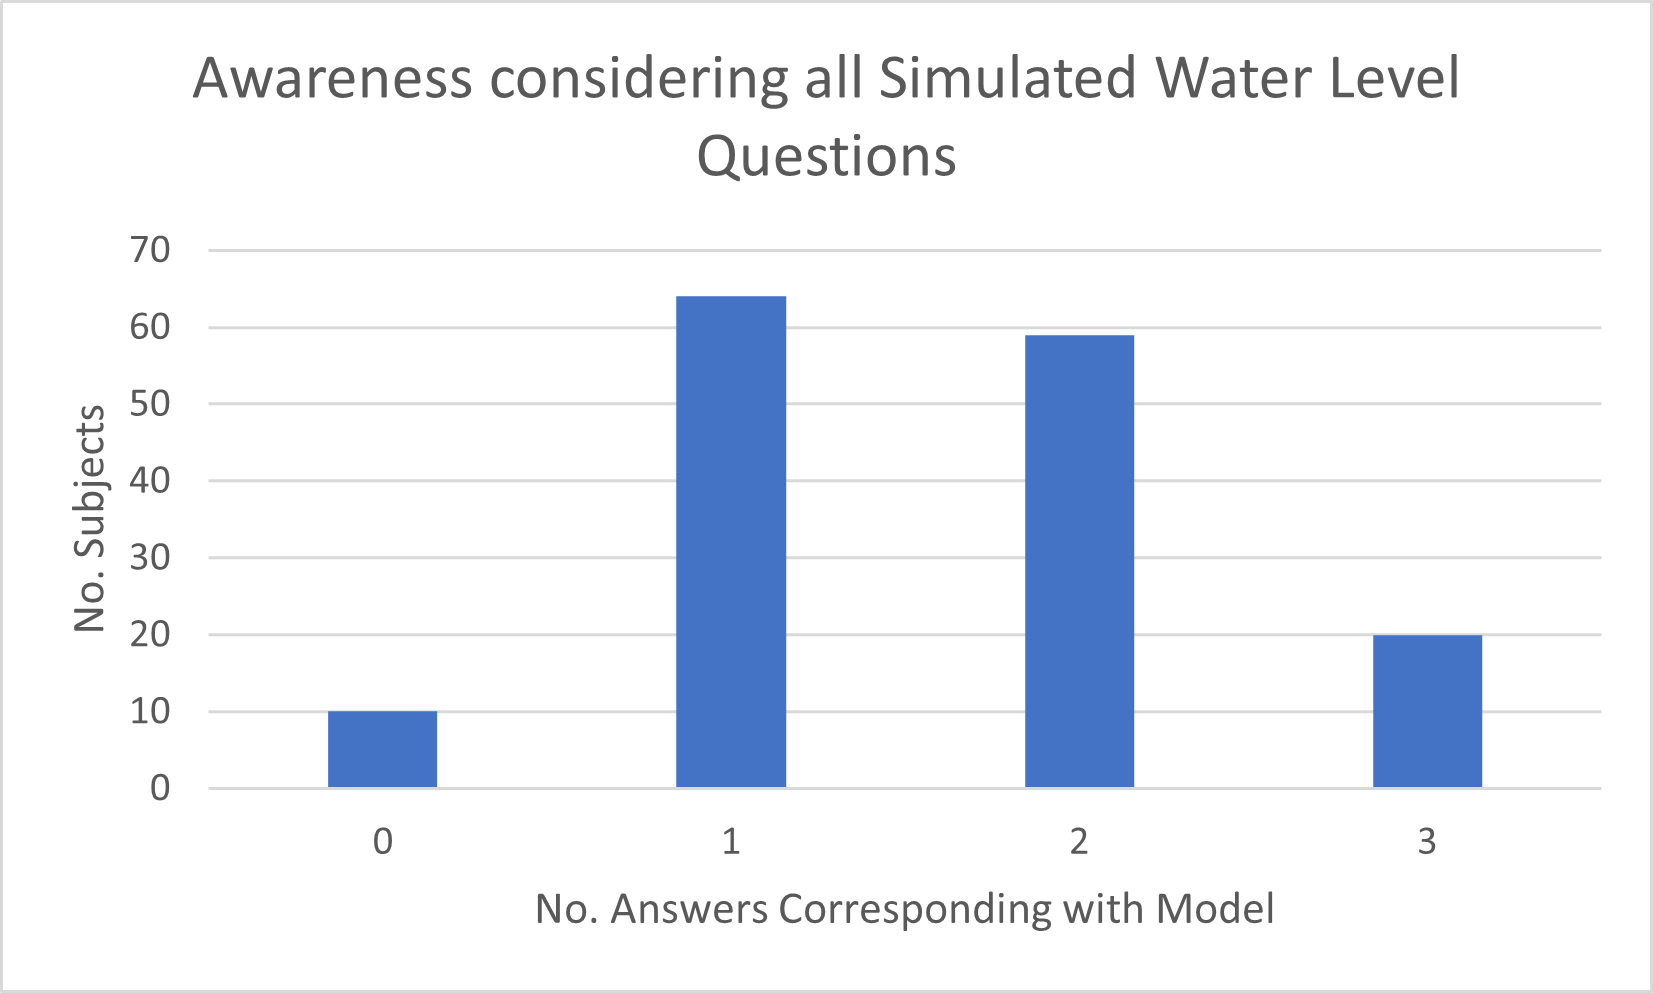
\includegraphics{fig_results/Awareness_ all_simulation_pictures_qs.png}
    \caption{Awareness considering all Visually Simulated Water Level Questions. 10 subjects had no answers corresponding with the models from (\cite{kartverket_se_2020}), 20 subjects responded with every answer corresponding with the model for these questions. 64 subjects responded to one of the four questions with answers which corresponded with the models. 59 subjects responded with 2 answers which corresponded with the models. }
    \label{fig:aware_all_edited_photo}
\end{figure}


The results here are more evenly spread than in figure 5.23, with the majority of subjects classing as somewhat aware.
\paragraph{}
 


\paragraph{}
As shown by the focus group there is issues with just requesting a numeric value from subjects. There is a higher potential connection for many individuals including another emotional layer when using pictures rather than numbers. 

\section{Factors Affecting Awareness}
  

\subsection{Shapiro Test Results}

During histogram analysis, only the factors of "interest-level" and "info-climate-sum" appeared normally distributed. To investigate whether these factors were truly normally distributed, a Shapiro test was carried out following (\cite{royston_extension_1982}).  An assumption of alpha value of 0.05 was determined meaningful (\cite{royston_extension_1982}). This means if the p-value created during this test is below 0.05 then the null hypothesis is rejected. This does leave a 5 \% chance of error. The results from the Shapiro test can be seen in Table 5.5 and this determines that none of the variables were normally distributed. 

\begin{table}[H]
    \centering
    \begin{tabular}{|l|l|l|l|}
    \hline
         \textbf{ Variable } &  \textbf{W-value}& \textbf{ P-Value}& \textbf{Distribution}\\ \hline
       Interest Level & 0.89332 & 4.343e-09 & Skewed \\ \hline
         Info Climate Sum  & 0.95721 & 0.0001159 & Skewed \\ \hline
        Flood Impact & 0.87779 & 6.681e-10 & Skewed \\ \hline
     \end{tabular}
    \caption{Shapiro Test Results. The alpha value was assigned 0.05, meaning that if the p-value is below 0.05 then the null hypothesis that this factor is not normally distributed was rejected. This leaves a 5 \% chance of error. Each of these factors p-value is below 0.05 meaning that their distribution was deemed skewed.Interest Level is when subjects self-identified their interest level in SLEs, ranging from professional interest to no interest. Info Climate Sum is the total of how many different sources subjects used to gather information about the climate. Flood impact is what the subjects predicted a flood in the place would impact them ranging from no impact to significant impact. }
    \label{table:shapiro_test_results}
\end{table}
\paragraph{}

This result that all variables and factors were skewed, including the important variable of awareness and interest level, influenced the choice of how to analyse dependency. As outlined in the method (chapter 3) Kruskal Wallis Rank Sum Tests were chosen due to the need to investigate multiple groups, upon one factor and having only measured each subject once.

\subsection{Kruskal Wallis Rank Sum Test}
The results from Kruskal Wallis Rank Sum Test conducted using the RStudio package based off \cite{hollander_nonparametric_2014} are outlined below.  An alpha value of 0.05 was chosen before these tests were carried out (\cite{hollander_nonparametric_2014}). This means there is a 5 \% chance of error when determining dependency of factors against the variable of awareness.
\paragraph{}
For clarity, the statistical labels for the Kruskal Wallis Rank Sum test are quickly outlined. For each of the results below, the p-value is the probability that measures the evidence against the null hypothesis.  If the p-value is lower than the selected alpha-value (0.05), then the null hypothesis can be rejected. The alternative way that the null hypothesis can be rejected utilises the H-value, which is the test statistic. If the \textit{df}, which stands for degrees of freedom, which is the number of groups within that factor, minus one, (\cite{minitab_interpret_2022}), is over four and the h-value is particularly high this can assist in the rejection of the hypothesis. Statistical interpretation used guidance from \cite{minitab_interpret_2022}.
\paragraph{}

Table 5.6 shows that, for the determination of awareness considering all questions on awareness, none of the factors were classed as dependent, when using the Kruskal Wallis rank sum test with an alpha value of 0.05. 

\begin{table}[H]
    \centering
    \begin{tabular}{|l|l|l|l|}
    \hline
         ~ & \textbf{awareness A} & ~ & ~ \\ \hline
        Factor &\textit{p}value &\textit{h}value & \textit{df} \\ \hline
           length of Knowledge & 0.73760 & 3.54770 & 6 \\ \hline
       Interest Level in SLE & 0.16920 & 6.43150 & 4 \\ \hline
        Concern about Climate & \cellcolor[HTML]{7df9ff} 0.05630 & \cellcolor[HTML]{7df9ff} 9.19960 & \cellcolor[HTML]{7df9ff} 4 \\ \hline
        Language of Survey & 0.2041 & 1.6129 & 1 \\ \hline
        Predicted Personal Impact of Flood & 0.7156 & 1.357 & 3 \\ \hline
    \end{tabular}
    \caption{Kruskal Wallis Test Results General Factors. "awareness A" means that for this determination of awareness, all five questions on awareness in the survey were included. Length of knowledge is how many years the subjects state they have knowledge of the places. Interest level in SLE represents the self-ranking of subjects from professional interest to no interest. Concern about Climate is self ranking of how concerned subjects are about climate change, from one to five. Language of survey, is whether the subjects chose to respond in Norwegian or English. Predicted Personal Impact of Flood is specifically for flooding in the research place and ranges from no impact to significant impact. }
    \label{kw_test_general_factors}
\end{table}

All the p-values were larger than the alpha value of 0.05. However, the p-value of Concern about Climate is 0.05630, highlighted in blue, is only just over.  If the alpha value was chosen to be 0.1, as is used in some studies (\cite{hollander_nonparametric_2014}), then this would be enough to reject the null hypothesis that concern about awareness is not dependent upon concern about climate. However, the h-value is exceptionally high and the \textit{df} is 4, meaning that, while not as confident as with a p-value rejection, the null hypothesis is still rejected (\cite{minitab_interpret_2022}). The result is that awareness appears dependent upon Concern about climate. 
\paragraph{}


Table 5.7 shows the Kruskal Wallis Test Results for the factors about the subjects community memberships. 


\begin{table}[H]
    \centering
    \begin{tabular}{|l|l|l|l|}
    \hline
         ~ & \textbf{awareness A} & ~ & ~ \\ \hline
        Factor &\textit{p}value &\textit{h}value & \textit{df} \\ \hline
        Sum of Community Memberships & 0.52060 & 4.20260 & 7 \\ \hline
        Marine worker & na & na & na \\ \hline
        Worker & 0.12310 & 2.37220 & 1 \\ \hline
        Resident & \cellcolor[HTML]{7df9ff} 0.01524 & 5.88900 & 1 \\ \hline
        Student & 0.55590 & 0.34691 & 1 \\ \hline
        Commuter & 0.44610 & 0.58063 & 1 \\ \hline
        Leisure User Land & 0.68790 & 0.16141 & 1 \\ \hline
        Leisure User water & 0.42120 & 0.64690 & 1 \\ \hline
        Other & 0.58620 & 0.29627 & 1 \\ \hline
    \end{tabular}
    \caption{Kruskal Wallis Test Results Community Membership. "awareness A" means that for this determination of awareness, all five questions on awareness in the survey were included. Sum of Community Memberships is how many communities did the subjects select in the survey. Marine worker is whether the subject considered themselves a marine worker. This had no responses. Community memberships also included worker, resident, student, commuter, leisure user land, leisure user water and other. The Other community membership was where the subjects self-identified their community: the most common response was tourist, with sailor coming next. }
    \label{kw_test_com_membership}
\end{table}
Resident is the only value which is highlighted in Table 5.7 as it is the only significant result when utilising a alpha value of 0.05. The factor of resident has a P-value of 0.01524, meaning the differences between the medians are statistically significant. This allows the rejection of the null hypothesis and the acceptance of the positive hypothesis that awareness is dependent on residency. 
\paragraph{}

Table 5.8 shows the Kruskal Wallis Test Results on the factors covering Information Sources for Place. Two forms of determining awareness are used as predictors. "awareness A", where all five questions on awareness in the survey were included and "awareness B", where only the questions which utilised edited photographs are used to determine awareness.

\begin{table}[H]
    \centering
    \begin{tabular}{|l|l|l|l|l|l|l|}
    \hline
       & \textbf{awareness A} & ~ & ~ & \textbf{awareness B} & ~ & ~ \\ \hline
       Factor &\textit{p}value &\textit{h}value & \textit{df} &\textit{p}value &\textit{h}value & \textit{df} \\ \hline
        Sum of Sources  & 0.44600 & 6.85110 & 7 & 0.45040 & 6.79650 & 7 \\ \hline
        Personal Observation & 0.22730 & 1.45790 & 1 & 0.36470 & 0.82162 & 1 \\ \hline
        Family & 0.78550 & 0.07406 & 1 & 0.81340 & 0.05572 & 1 \\ \hline
        Friend & 0.27580 & 1.18780 & 1 & 0.30200 & 1.06520 & 1 \\ \hline
        Newspaper & 0.74490 & 0.10583 & 1 & 0.48500 & 0.48765 & 1 \\ \hline
        TV & 0.87330 & 0.02542 & 1 & 0.33420 & 0.93237 & 1 \\ \hline
        Social Media & 0.48540 & 0.48671 & 1 & 0.95090 & 0.00379 & 1 \\ \hline
        Membership of Organisation  & 0.67530 & 0.17550 & 1 & 0.70980 & 0.13848 & 1 \\ \hline
        Municipality & 0.82590 & 0.04839 & 1 & 0.12790 & 0.57600 & 1 \\ \hline
        \hline
    \end{tabular}
    \caption{Kruskal Wallis Test Results: Information Sources for Place as Factor.  "Awareness A" means that for this determination of awareness the three questions on awareness utilising edited photographs were included, which display awareness of the tide and present and future storm surges.  "Awareness B" excludes the future storm surge response and only considers the present storm surge and tide.  The sum of sources is the total number of sources each subject selected as where they gather information about place from. These sources are personal observation, family, friend, newspapers, TV, social media, via membership of organisations and the Municipality. }
    \label{kw_test_info_place}
\end{table}

There were no significant values, meaning that for each of these hypotheses the null hypotheses was accepted.
\paragraph{}
Table 5.9 shows the Kruskal Wallis Test Results on the factors Information Sources for Climate. As with Table 5.8, two determinations of awareness are used as predictors.



\begin{table}[H]
    \centering
    \begin{tabular}{|l|l|l|l|l|l|l|}
    \hline
        & \textbf{awareness A} & ~ & ~ & \textbf{awareness B} & ~ & ~ \\ \hline
        Factor &\textit{p}value &\textit{h}value & \textit{df} & \textit{p}value &\textit{h}value & \textit{df} \\ \hline
        Sum of Sources & 0.91220 & 3.32660 & 8 & 0.45218 & 8.12040 & 8 \\ \hline
        Personal Observation & 0.11750 & 2.45020 & 1 & 0.24550 & 1.34870 & 1 \\ \hline
        Family & \cellcolor[HTML]{7df9ff} 0.00481 & 0.94470 & 1 & 0.56970 & 0.32313 & 1 \\ \hline
        Friend & 0.82460 & 0.04910 & 1 & 0.63010 & 0.23186 & 1 \\ \hline
        Newspaper & 0.09036 & 2.86790 & 1 & \cellcolor[HTML]{7df9ff} 0.01218 & 6.24830 & 1 \\ \hline
        TV & 0.61230 & 0.25689 & 1 & 0.75000 & 0.10154 & 1 \\ \hline
        Social Media & 0.74950 & 0.10960 & 1 & 0.92830 & 0.00809 & 1 \\ \hline
        Membership of Organisation & 0.30270 & 1.06220 & 1 & 0.27500 & 1.91500 & 1 \\ \hline
        Peer Reviewed Publications  & 0.88040 & 0.02650 & 1 & 0.12390 & 2.36760 & 1 \\ \hline
        Formal Education & 0.64850 & 0.20779 & 1 & \cellcolor[HTML]{7df9ff} 0.02438 & 5.06770 & 1 \\ \hline
    \end{tabular}
    \caption{Kruskal Wallis Test Results Variables on Information Sources for Climate. "Awareness A" means that for this determination of awareness the three questions on awareness utilising edited photographs were included, which display awareness of the tide and present and future storm surges.  "Awareness B" excludes the future storm surge response and only considers the present storm surge and tide.  The sum of sources is the total number of sources each subject selected as from where they gather information about changes to the climate. These sources are personal observation, family, friend, newspapers, TV, social media, via membership of organisations, peer reviewed publications and formal education. The values highlighted in blue are statistically significant. }
    \label{kwtest_info_climate}
\end{table}

For the determination of awareness which considered all five possible questions, Family is a significant factor. This means that this determination of awareness appears dependent on family as a sources of observation. This result is discussed later in the context that 25 subjects have a personal connection to the researcher.
\paragraph{}
For the determination of awareness which only utilised the edited photograph questions, both the information source of newspaper and formal education were significant.
\paragraph{}
Table 5.10 shows the Kruskal Wallis Test Results on the factors of Place subjects responded on. These places had varied physical vulnerability as outlined in Table 2.1 in the background.

\begin{table}[H]
    \centering
    \begin{tabular}{|l|l|l|l|l|l|l|}
    \hline
~ & \textbf{awareness A} & ~ & \textbf{awareness B} & ~ &  \\ \hline
        Factor &\textit{p}value &\textit{h}value & \textit{df} &\textit{p}value &\textit{h}value & \textit{df}\\ \hline
         Brattøra & 0.1044  & 2.6364 & 1 & 0.771 & 0.084739 &1\\ \hline
        Grillstad & 0.1815 & 1.7855 & 1 & 0.1565 & 2.008 & 1 \\ \hline
       Skansen & 0.09349 & 2.8133 & 1 & 0.05527 & 3.6738 & 1\\ \hline
         Nidelva & 0.2472 & 1.3388 & 1 & 0.9523 &  0.0035714 & 1\\ \hline
    \end{tabular}
    \caption{Kruskal Wallis Test Results: Place as Factor. "Awareness A" means that for this determination of awareness the three questions on awareness utilising edited photographs were included, which display awareness of the tide and present and future storm surges.  "Awareness B" excludes the future storm surge response and only considers the present storm surge and tide.  Brattøra, Grillstad, Skansen and Nidelva are the places considered.}
    \label{kwtest_place}
\end{table}
None of the factors of each of the places have a statistically distinct median. This means the null hypothesis is accepted and awareness is not considered dependent on the variable of place. 
  How the non-parametric hypothesis testing of Kruskal Wallis Rank Sum tests relate to the original hypotheses it outlined at the end of the discussion section.   
\paragraph{}

  










% LIMITS OF SURVEYING AS TECHNIQUE
% COMMUNICATION RISK - REACHING OUT TO SUBJECTS
%LIMITS OF EDITED PHOTOS
% HOW TO CREATE A FRAMEWORK
%LIMITS OF RESULTS - E.G. CODING /STATS LIMITS
%LIMITS OF SURVEYING AS TECHNIUE 
%LACK OF INTERVIEWS
%PEOPLE ONLY TICK ONE BOX WHEN ASKED CERTAINS QS E.G. COMMUNITY MEMEBERSHIP
%LESSONS LEARNED FOR REPEATING

%size of city plus no major disaster impacts results and discussion
%seasonal aspect

%remember survey was difficult - can say quite aware even if only got 2 correct

%issue comparing norwegian and english surveys - word just dont mean the same - direct translation is impossible -cultural differences when viewing risk

\cite{cutter_community_2020} discusses difference between insurance and resilience - how economic resilience can be impacted at lower levels of flooding impact

\chapter{Discussion of Results}

\section{Research Question 1 - How resilient will Trondheim to be to SLEs during 2022 to 2050 and 2050 to 2100? }

From the literature review Trondheim's natural systems of resilience and technological systems of resilience can be considered very high for the period of 2022 to 2050. From the results of the survey the  social systems of resilience for this period are only considered as medium as the awareness determined for the current SLEs are only somewhat. Overall Trondheim's resilience to SLEs can be considered high, due to the limited damage potential and the high level of resources available to deal with it. However this does not mean that there is not potential economic, cultural or social impacts. Just that it is projected that the daily activities occurring in Trondheim will quickly return to normality after the likely sea level extreme events during this period.
\paragraph{}
The awareness determined for SLEs in 2090 is higher than the awareness for 2022. This allows for the projected social system resilience for the period of 2050 to 2100 to be high. The technological system resilience is also considered as high for this period and the natural system resilience is considered medium. Overall the projected resilience for Trondheim to SLEs during 2050 to 2100 is high. However, projected resilience is an highly dynamic meaning that the resilience of a place will change over time. There is requirements from the Sendai framework for and the UN sustainable developments goal 11 and 13 that cities resilience to natural hazards should increase \cite{gonzalez-riancho_storm_2017}. To see if this is occurring repeated measurements of resilience is required. 

This determination of current resilience levels is backed up by \cite{opach_seeking_2020}. Who conducted a cluster analysis of community resilience for Norway and ranked Trondheim as having high economic, housing and infrastructure resilience. They were designated with lower institutional and community capital decreasing the social system resilience. However it can be argued that the way these valuations for resilience were determined were biased against cities as and favoured less populous areas.

\paragraph{}
This requirement of increasing resilience brings up the question of what level of resilience should a place have? What level is acceptable to stakeholders is suggested as a method of answering this question by \cite{gerkensmeier_governing_2018}. The four research sites of Skansen, Grillstad, Brattora and Nidelva represent the most vulnerable places in Trondheim to SLEs. Taking the extreme potentials of SLEs, helps minimise the chance of overestimating the resilience Trondheim has to SLEs. The results from the survey indicate that the place had no impact on how aware subjects were to SLEs, even though each of these places had different level of natural and technological system resilience. 




\section{Research Question 2 - Are Stakeholders aware about changes to SLEs?}
%people are somewhat aware


\section{Research Question 3 - What factors impact stakeholders' awareness of SLEs? }
%more difficult as not so many aware
%could try and reverse it - what makes people unaware 
%interest level doesn't appear to be a factor in awareness which contrast with 


The choice which format method to use while asking about sea level changes is likely to have an influence on how participants perceive this change. For example considering change as metres in height vs area of land influenced may results in different perceptions of the changing risks and potential impacts.  By sticking firmly in the realm of historical fact and scientific models with these questions there has been an attempt to investigate awareness of SLEs rather than perception. 

\section{Visualisation of sea level change}
Discuss exclusion of questions "How much do you think the sea level will change in the next 30 years?" and "How much do you think the sea level has changed here in the past 30 years?". 

Especially why focus on answers which were picture based versus answers that were number based


%EDUCATION AS AN OPTION WAS ONLY ADDED AFTER day 1
%as was peer reviewed articles for the norwegian options
%so first 20 respondents did not have that option

\section{Awareness vs Assumed Awareness}
Discuss lack of awarenes, particularly in groups who could be assumed to be aware of risk

e.g. graphs - interest level vs determined awareness (ss-aware-all or ss-aware)

do highlight lack of marine workers who responded while disucssing this. 

\section{Risk Perception - Personal Impacts of SLEs and associated Flooding}
There was opportunity for subjects to give extra information on certain topics as can be seen in the appendix. From these responses narratives about perception of risk can be explored. For example their was a very varied response to "How would flooding associated with SLEs in this area affect you? If you would like to give more details on this, please write below." This has been grouped into narratives depending on the impact level the subjects gave to the previous question.
\paragraph{}

Subjects who felt they would have no impact who gave more details either stated that they lived far from the sea, or that they would be moving away soon. This highlights an idea that if the sea level extreme does not impact items they own or their daily activity that it will not affect them at all. Nuisance flooding was not considered an issue, nor how flooding could impact key infrastructure for example transport connections. One subject gave details of how flooding did impact where they normally park their car, but as it wasn't parked during this event then they weren't impacted. 
\paragraph{}

Subjects who responded that flooding in this area would have mild impact and gave more information gave a wider range of responses than those who felt it would not impact them. The overall narrative was that flooding won’t affect where they live, but may impact their family and their activities. One curious response was from an individual who said that because they lived on a higher floor they would not be impacted. Living on a higher floor may provide some protection but in a extremely high sea level could still have impacts on daily activities. This continues the narrative that SLEs may impact my activities but as long as it doesn't negatively impact my possessions the impact can be considered mild. This raises questions about what it means to experience a flooding hazard. What it means to have direct experience can have varied definitions. 
\cite{whitmarsh_are_2008} defines direct flooding experience as those who have experienced forms of flood damage to their home, garden or vehicle within the last half decade. This is a particularly tight definition of direct experience and focuses on ownership. People who do not own a home, garden or vehicle can still be impacted by flooding and their experience may be very different.  
\paragraph{}
It is commonly assumed that direct experience makes people more concerned about climate change and its potential personal impacts\cite{lujala_role_2020}. However this does not always appear to be the case \cite{lujala_role_2020}. Perhaps some of this variation is due to variation in what is defined as direct experience. Further research could look into differing types of direct experience. 
\paragraph{}
Only once subjects responded with medium impact did a negative emotional response get expressed. Subjects discussed how flooding will affect places where they stored things, particularly at the harbour. Subjects who ranked flooding in this area as Significant impact gave similar response. The overall narrative expressed from the extra information given here is that subjects appear to believe that if SLEs do not affect the metres of where they live it wont affect them. 
\paragraph{}
None of the subjects who gave extra information mentioned insurance as a factor in their perception of personal impact level of flooding due to SLEs. GonZalex-Riancho et al, 2017 in \cite{gerkensmeier_governing_2018} says that stakeholders for the Wadden Sea Region a similarly developed area in Northern Europe, who has a longer history of negative flooding impacts from SLEs, reject that insurance can be considered as a form of disaster risk management. Perhaps the self-selecting stakeholders for Trondheim have similar views. How economists view the role of insurance in the case of resilience to flooding often does not correspond with other stakeholders, particularly residents \cite{gerkensmeier_governing_2018}.

There is widespread insurance of buildings in Norway against damage from natural hazards \cite{lujala_role_2020}. Households with fire insurance are required to also have insurance for the damage caused by landslides, storms and flooding. The cost of this is connected to the insurance rate for fire damage and is not dependent on the location of the house \cite{lujala_role_2020}. The role of insurance and the welfare state in the perception of risk in Trondheim is likely significant \cite{lujala_role_2020}, but this was not mentioned by any of the subjects regardless of their perception of the potenital personal impact of flooding in these places. Future research could include questions to gain a greater understanding of how stakeholders view the role of the welfare state or insurance policies in their perception of this risk. 






\section{Information sources and fear of natural hazard }
Mentioned several times by subjects in the extra information responses is the risk of the from land falling away. This concern about this risk is highlighted in the quote below from a subject who ranked the impact of flooding the area as significant.

\begin{itemize}
    \item "A few days ago, I saw a video of some part if Norway where an entire chunk of land just went under the water, I guess due to erosion, and I would assume that storm surges have an effect on erosion. That video was horrifying and I keep thinking, if something like that to happen here in Trondheim, which part of coast would it take away. I would love to buy/rent a house near the coast, but after watching that, I am not so sure."
\end{itemize}
\paragraph{}

At a surface level this quote highlights a fear of flooding and that they like other subjects who labelled their impact as no impact will avoid living near the coast in part due to fear of flooding. But taking it further the fear here isn't simply of SLEs but of land falling away. 
\paragraph{}

This fear of land falling away is brought up by several subjects at multiple points when given the opportunity to broaden the survey. For example when asked "If you would like to give other examples of risk in this area, please write here." by far the most common response was risk of landslide - often specifically due to quick clay. This response was mainly given by those taking the survey in Norwegian. 
\paragraph{}
*EXPAND**quick clay and landslides get media attention - how does this impact awareness and resilience...
\paragraph{}

Other responses focused around lack of housing, because people will have to move. This view is the flip side of the many respondents who stated that they will minimise personal impact of flooding due to SLEs by not residing along the coast. 
Trondheim has 34.6 percent of the land use in its coastal area influenced by buildings \cite{engebakken_construction_2022}, a significant percentage which are residences. The impact to housing in Trondheim is likely not that significant within the next 70 years, but the impact in the desire to live their may be significant. This push inland could have significant economic, social and ecological impacts in Norway. 
\paragraph{}


%Experience types (of flooding) - damaged belongings, survived, nuisance, direct observation, family/friend observation, heard about e.g. media

\section{Limitations of single-risk, single-scale risk analysis}
There is an increasing demand for multi-risk, multi-scale, multi-stakeholder determination of risk and resilience \cite{gerkensmeier_governing_2018} and \cite{cutter_community_2020}. An attempt has been made to display a method for quickly and cheaply determining social resilience utilisng the views of many stakeholders. There is limitations to this results of Trondheim being considered resilient as it is dependent only on the risk from SLEs. As highlighted by the subjects, there are other risks including risk of landslides. Landslide due to quickclay are also impacted by weather conditions, much like SLEs. 
\paragraph{}

While Trondheim is considered to currently have projected resilience for SLEs for the period of 2022 to 2050 and 2050 to 2100, this does not mean that normality will quickly be returned to if multiple other incidents occurred at the same time. These other risks could be natural hazards or caused by human choice. 

\section{Limitations of Technique}
The COVID-19 pandemic provided significant limitations to this research. This was the main factor in the decision to only use surveys and not complement with interviews. Furthermore, resilience is dynamic and will have been affected by the pandemic. 
\paragraph{}
The data collection limitations include the number of subjects and the impact of only surveying during the summer. The lack of marine workers within the subjects is a major limitation of this study, but does not prevent an overview of local knowledge. Particularly important is the limitation of only having the results for one year, which creates a snapshot of resilience rather than considering how it is changing overtime.  The exclusion of Nyhavvna as a research site is a limitation, which could be corrected in a repetition of this research.  The final limitation is the analysis technique which was limited due to the skewed distribution of the survey results.




\section{bits cut from results }
Trondheim city plans indicate that the research sites should be prepared for 4.87m by 2100.



Table 5.2 shows that the most popular place for responses was Nidelva.Nidelva is the most central of the locations and has the greatest daily throughput of people. It also includes perhaps the most iconic views of Trondheim.
  Next popular was Grillstad, perhaps due to the recognition by residents that the area could be severely influenced by flooding from SLEs. Skansen and Brattøra are the next most responded to, both of these locations have significant commercial ventures. Brattøra in particular is dominated not by residency but by offices and industry. Perhaps the conduction of this survey in Summer decreased the number of responses due to the lack of office workers. Almost evenly split for each location was whether the survey was completed in Norwegian or English. English surveys had 66 response, while the Norwegian survey had 87 responses.  


  Awareness as a facet of local knowledge was the key variable within this project. The purpose of the survey was to allow for the determination of awareness in Trondheim of SLEs. An interesting comparison is the level of interest against awareness. There is the assumption that high or professional interest in SLEs is associated with higher levels of awareness of the risk. 


  There is no linearity or other pattern observed in Figure 5.11. This raises questions about the assumption of resilience due to the presence of professionals within a community. However, there is a serious limitation: no marine workers were identified in the survey subjects. Subjects who ranked their interest in sea level as high (4) had the largest variation in determined awareness according to the number of answers they gave which matched models from \cite{kartverket_se_2020}. 


  How memory is formed and how it impacts awareness and resilience is a highly debated field \cite{de_guttry_expiry_2022}.

  The lack of memory is interesting considering that length of knowledge for 95 out of 153 subjects the majority included at least one sea level extreme events as can be seen in the figure below. 


  While access to survey does not appear to have influence on awareness of local knowledge, the results are important for the discussion on how to create a framework for determining resilience of a place.

   However almost all subjects only chose one access type as seen 5.15

The key result for future research is that data collection using posters was a popular access method. 50 posters were printed. To see the communication design principles influence on the poster design, you can find it attached in the appendix. These posters were split evenly between the research sites and half were placed at the start of data collection and the other half after the first month. The results shown in figure 5.16 are again influenced by the subjects tendency to tick only one box, when there was the option to tick several. For example, it is known that many of the subjects who have personal connections to the researcher actually accessed the survey via social media or organisational membership. This tendency and its influence on the results is expanded upon in the discussion of results and the discussion of framework.
% DISCUSSION  related to the reproducibility of this technique

\section{Demographics}
The purpose of this research is to assist in the creation of a framework to determine resilience of a place, specifically to sea level extremes. This is to allow repeated measurements of resilience to determine whether a place is making improvements in its resilience. How resilience is improved is done through many techniques including......

Resilience and vulnerability are impacted by demographic variables \cite{rod_integrated_2012}, but improving of resilience shouldn't be done by changing population demographics. Arguing a place is resilient simply due to their being a high percentage of women, or immigrants, or the age of the population is not a use full nor moral lens in which to discuss improvements to resilience. It can be useful to highlight areas or groups who are particularly vulnerable, but not forcing those groups to disperse against their will. For this reason standard demographic questions were not part of this survey. Subjects attributes which local governance could reasonably, cost effectively and most importantly morally impact were prioritised as research variables over demographics. 

Furthermore by asking questions upon gender and age can influence how subjects answer these questions.*citation needed*

Awareness or a hazard is not determined by gender, even if gender can correlate with it.  Gender was determined not a key variable from literature review before the creation of the survey. This is the same for the majority of demographic variables which were not investigated during this research.

Certain demographic questions can be answered by inferring from the results to key questions. For example language skills and even immigration status can be inferred from the subjects decision to complete the survey in Norwegian or English. The lack of availability of the survey in other languages is a limiting factor. Percentage of the population who do not have a reasonable understanding of either Norwegian or English in Trondheim is ****. For this reason plus limitations of funds, researcher skills and time it was deemed acceptable for the posters, emails, social media, website and surveys to only be available in Norwegian and English. However, if this was to be repeated in other locations or nationally this would need to be reconsidered. 

The key demographic that was considered was interest level and professional experience with sea level extremes. ***** highlights that those with professional experience of the relevant hazard or have professional interest are more aware and hence improve an places resilience to the specific hazard. Unfortunately even with an extended deadline marine workers were not an included part of this research. There is a small percentage who have professional interest in sea level extremes see table** below. 

\begin{table}[!ht]
    \centering
    \caption{Interest Level of Subjects in Sea Level Extremes}
    \begin{tabular}{|l|l|l|l|l|}
    \hline
        Not & Low & Medium & High & Professional \\ \hline
        1 & 2 & 3 & 4 & 5 \\ \hline
        8 & 22 & 71 & 40 & 12 \\ \hline
    \end{tabular}
\end{table}

As can be seen above the majority have medium level interest in sea level extremes. The spread of results to this question is approximatley normal, which could be seen as either that a good spread of subjects were contacted. However whether this does correctly model Trondheim's population level of interest in the subject is not very likely.  Survey participants were self selecting so that subjects have volunteered their time even with low or no interest in the research is helpful, but it is to be expected that people with an interest in a subject are more likely to take part in a survey.

This has been attempted to be minimised by making the survey as short and as easy to do as possible and by utilizing the researchers network. For more discussion on the careful utilisation of the researchers network to reach subjects who could have been missed find it under the section Survey Access. 

\section{Survey Access}

\begin{table}[!ht]
    \centering
    \caption{Access to Survey}
    \begin{tabular}{|l|l|l|l|l|l|}
    \hline
      poster & email & social media & via organisation membership & via place of employment & personal connection to researcher \\ \hline
        1 & 2 & 3 & 4 & 5 & 6 \\ \hline
        70 & 2 & 48 & 2 & 4 & 24 \\ \hline
    \end{tabular}
\end{table}


%This is the Summary
%%=========================================
%Here you give a summary of your your work and your results. This is like a management summary and should be written in a clear and easy language, without many difficult terms and without abbreviations. Everything you present here must be treated in more detail in the main report. You should not give any references to the report in the summary -- just explain what you have done and what you have found out. The Summary and Conclusions should be no more than two pages.



\chapter{Conclusion}

It is generally accepted that sea level extremes are becoming more frequent globally thus far resilience research often focuses on, highly vulnerable locations. However looking more closely at an area which is regarded as less can help create a reference point or target for a locations place-based resilience.

Much of Trondheim's infrastructure and population is situated within the coastal zone (figure \ref{fig:research_site}), as is common in Norway. To understand Trondheim's changing resilience to sea level extremes, its technological, natural and social systems resilience were considered.  Projected resilience was viewed as a projected outcome, which can be determined by analysing the systems which impact the risk (section \ref{theory-resilience}). In this case social, natural and technological, systems impacting the risk of sea level extremes. 
\paragraph{}

Literature reviews, investigation of the coastline, analysis of city plans and planning permissions were used to determine Trondheim's natural and technological systems resilience (section \ref{data-sources}). Online surveys of stakeholders were used to aid the determination of Trondheim's social system resilience, specifically investigating the key variable of awareness (section \ref{data-collection}). Awareness is an important theme in this thesis falling under the broader concept of local knowledge, which in turn falls under the concept of social system resilience (section \ref{theory-resilience}). A place-based understanding of community was used in this conceptualisation of social system resilience due to its dominance in Norwegian politics (section \ref{theory-resilience}). This framework was designed based on feedback received from a focus group and a pilot study that carefully considered the framing of textual and visual communication, particularly the use of edited photographs to display likely future scenarios of sea level extremes in Trondheim (section \ref{data-collection}). Four places within Trondheim - Skansen, Grillstad, Brattøra and Nidelva - were selected as study areas to investigate the city's resilience. They were chosen after after naturalistic observation due to their higher physical vulnerability to SLEs and large daily throughput of people which included a broad representation of society.

\paragraph{}
This thesis determines Trondheim's projected resilience to SLEs in the 2022-2050 period as high (section \ref{RQ1-findings}), while the projected resilience for 2050-2100 is determined to be very high (section \ref{RQ2 - findings}). These high values of projected resilience are mainly due to a the large improvement of the technological systems outlined in the cities plans and building requirements (\ref{tech-resilience-discussion}), while the social and the natural systems show a slight reduction  in the projected resilience for the same time period (section \ref{RQ2 - findings}). Resilience is highly dynamic and over the extended time frame considered in this thesis (2022-2100) these results are likely to change. Hence the requirement for designing a framework for repeated measurements to determine the trend of a places resilience as was attempted here. By considering the trend we can determine whether Trondheim is inline with the United Nations Sustainable Development Goals (UN SDG’s) 11 and 13 requirement of improving resilience of human settlements.

\paragraph{}
Stakeholders were deemed somewhat aware about changes to SLEs (section \ref{RQ3 - finding}). The factors deemed to have impact on stakeholders' awareness of SLEs are whether they are residents, or whether they utilise the sources of family, newspapers and formal education for their information on climate change. This result enforces the importance of framing the textual and visual communication for the designated audience as outlined in the communication design section of the methods as this can impact awareness and perception.  The method used to collect data on awareness was deemed appropriate. There is room for improvement in the data analysis technique of determining awareness. Neither subjects self-ranked interest level, nor the place they chose to respond upon, were factors which were deemed to impact awareness.
\paragraph{}



Whether the surveys utilising visual simulations of sea level extremes to determine Trondheim's social system resilience to SLEs can also be used to improve awareness, hence improving resilience, would be an interesting avenue for future research. As is the impact on the research of including sectors of society who are often non-deliberately excluded from such research, for example by only utilising volunteer based stakeholder workshops, but can be the most vulnerable including migrants, short term residents, tourists, youth and the immune compromised. Improving resilience is a requirement of the Sendai framework and the United Nations Sustainable Development Goals 11 and 13. This thesis has shown that carefully designed surveys may be a useful tool in a framework designed to repeatedly measure resilience to see whether these goals are being met.



%include bibliography
\addcontentsline{toc}{chapter}{Bibliography}
\printbibliography

% Include more chapters as required.
%%=========================================
\appendix
%This is Appendix A - Acronyms
%%=========================================

\chapter{Acronyms}
\begin{description}
\item[df]degrees of freedom
\item[GIA] glacioisostatic adjustment
\item[No.] Number of
\item [RStudio] RStudio Version 2022.02.3+492 on Windows Desktop
\item[SLEs] Sea Level Extremes
\item [UN SDGs] United Nations Sustainable Development Goals 
\end{description}

Note that if there is a variation in English spelling the British English variation was selected in line with the Cambridge Dictionary. For SI units the UK metric organisation style guide was followed https://ukma.org.uk/style-guide/.  

The code used can be found in the github repo: 
%%This is an Appendix
%%=========================================

\chapter{Hypotheses, Summary Statistics, Visual Communication}

%%=========================================
\section{Hypotheses}

\subsection{Hypothesis dependent on community membership}
\begin{enumerate}
    \item We expect residents to be aware
    \item We expect commuters to be aware
    \item We expect marine workers to be aware
    \item We expect non-marine workers to be unaware
    \item We expect water leisure users to be aware
    \item We expect land leisure users to be unaware
    \end{enumerate}
\paragraph{}

\subsection{Hypothesis dependent on local knowledge}
\begin{enumerate}
    \item We expect subjects with professional interest in SLEs to be aware
    \item We expect subjects with primary knowledge about places which are on reclaimed land to be aware
    \item We expect subjects with a length of knowledge greater than 20 years of the area to be aware
    \item We expect subjects with a length of knowledge less than 1 year of the area to be unaware
    \item We expect subjects with many information sources about the place to be aware
    \item We expect subjects who chose to respond in Norwegian to be aware
\end{enumerate}
\paragraph{}

\subsection{Hypothesis dependent on awareness of changing climate}
\begin{enumerate}
    \item We expect subjects with many information sources about climate change to be aware
    \item We expect subjects with the information source of formal education to be aware
    \item We expect subjects with the information source of peer reviewed published papers to be aware
    \item We expect subjects who are more concerned about climate change to be aware
    \item We expect subjects who predict they will be impacted by flooding from SLEs to be aware
\end{enumerate}

\section{Summary Statistics }
Find below table \ref{table:summary_stats} which details the summary statistics for the responses to the survey. Table \ref{table:variable to questions} contains the codified variable name and what questions they respond to.



\begin{center}
\begin{table}[H]
    \centering
    \begin{tabular}{|l|l|l|l|l|l|l|}
    \hline
        variable name & mean & Std Dev. & min & max & range & skew  \\ \hline
        long\_know & 3.24 & 1.60 & 0 & 6 & 6 & 0.23 \\ \hline
        com\_mem & 1.44 & 0.89 & 0 & 6 & 6 & 2.10  \\ \hline
        com\_marine\_worker & 0.00 & 0.00 & 0 & 0 & 0 & Na   \\ \hline
        com\_worker & 0.12 & 0.33 & 0 & 1 & 1 & 2.26  \\ \hline
        com\_resident & 0.46 & 0.50 & 0 & 1 & 1 & 0.17  \\ \hline
        com\_student & 0.25 & 0.44 & 0 & 1 & 1 & 1.11 \\ \hline
        com\_play\_land & 0.27 & 0.45 & 0 & 1 & 1 & 1.00   \\ \hline
        com\_play\_water & 0.11 & 0.32 & 0 & 1 & 1 & 2.45  \\ \hline
        com\_commuter & 0.10 & 0.31 & 0 & 1 & 1 & 2.56   \\ \hline
        com\_other & 0.12 & 0.32 & 0 & 1 & 1 & 2.35   \\ \hline
        interest\_level & 3.17 & 0.95 & 1 & 5 & 4 & -0.16 \\ \hline
        ss\_now & 0.39 & 0.49 & 0 & 1 & 1 & 0.44  \\ \hline
        ss\_future & 0.31 & 0.46 & 0 & 1 & 1 & 0.83 \\ \hline
        ss\_tide & 0.88 & 0.32 & 0 & 1 & 1 & -2.35 \\ \hline
        info\_place\_sum & 1.94 & 1.34 & 0 & 8 & 8 & 1.61 \\ \hline
        info\_climate\_sum & 3.50 & 1.72 & 0 & 8 & 8 & 0.24 \\ \hline
        worry\_climate & 4.03 & 1.15 & 1 & 5 & 4 & -1.17 \\ \hline
        flood\_impact & 2.50 & 0.89 & 1 & 4 & 3 & 0.04  \\ \hline
        slr\_past & 0.17 & 0.43 & 0 & 2 & 2 & 2.47  \\ \hline
        slr\_future & 2.33 & 0.69 & 0 & 3 & 3 & -1.26 \\ \hline
        ss\_event & 0.58 & 0.93 & 0 & 7 & 7 & 2.78  \\ \hline
        survey\_access & 2.55 & 1.84 & 0 & 6 & 6 & 0.79  \\ \hline
        language & 0.57 & 0.50 & 0 & 1 & 1 & -0.27  \\ \hline
        place\_brattøra & 0.20 & 0.40 & 0 & 1 & 1 & 1.52  \\ \hline
        place\_grillstad & 0.24 & 0.43 & 0 & 1 & 1 & 1.19 \\ \hline
        place\_nidelva & 0.37 & 0.49 & 0 & 1 & 1 & 0.52 \\ \hline
        place\_skansen & 0.19 & 0.39 & 0 & 1 & 1 & 1.57 \\ \hline
    \end{tabular}
    \caption{Summary Statistics}
\label{table:summary_stats}
\end{table}
\end{center}


\begin{center}
\begin{table}[H]
    \centering
    \begin{tabular}{|l|l|}
    \hline
        variable name  & question asked \\ \hline
        long\_know & How long have you known this area? \\ \hline
        com\_mem  & What communities in this area are you part of? \\ \hline
        com\_marine\_worker & "" \\ \hline
        com\_worker & "" \\ \hline
        com\_resident & "" \\ \hline
        com\_student & "" \\ \hline
        com\_play\_land & "" \\ \hline
        com\_play\_water &  "" \\ \hline
        com\_commuter &  "" \\ \hline
        com\_other &  "" \\ \hline
        interest\_level & What is your level of interest in sea level extremes? \\ \hline
        ss\_now  & Which image shows the current 20-year storm surge? \\ \hline
        ss\_future  & Which image shows the 20-year storm surge projected for 2090? \\ \hline
        ss\_tide  & Which image displays the current high tide? \\ \hline
        info\_place\_sum & Where do you get information about changes to this place? \\ \hline
        info\_climate\_sum &  "Where do you get information about changes to the climate" \\ \hline
        worry\_climate &  Are you concerned about climate change? \\ \hline
        flood\_impact &  How would flooding associated with sea level extremes in this area affect you? \\ \hline
        slr\_past & How much do you think the sea level has changed here in the past 30 years? \\ \hline
        slr\_future & How much do you think the sea level will change in the next 30 years? \\ \hline
        ss\_event & Please tick if you remember any of these dates when coastal  \\ \newline
        & sea levels in Trondheim were over 2m \\ \hline
        survey\_access  & How did you access this survey? \\ \hline
        language  & Determined from which survey subjects filled out \\ \hline
        place\_brattøra  & "" \\ \hline
        place\_grillstad  & "" \\ \hline
        place\_nidelva & "" \\ \hline
        place\_skansen & "" \\ \hline
    \end{tabular}
    \caption{Variable link to Survey Question}
\label{table:variable to questions}
\end{table}
\end{center}


\begin{center}
\begin{table}[H]
    \centering
    \begin{tabular}{|l|l|l|l|l|l|l|}
    \hline
        variable name & mean & Std Dev. & min & max & range & skew  \\ \hline
        info\_place\_sum & 1.94 & 1.34 & 0 & 8 & 8 & 1.61 \\ \hline
        info\_place\_po & 0.73 & 0.45 & 0 & 1 & 1 & -1.00  \\ \hline
        info\_place\_family & 0.10 & 0.31 & 0 & 1 & 1 & 2.56 \\ \hline
        info\_place\_friend & 0.19 & 0.39 & 0 & 1 & 1 & 1.57  \\ \hline
        info\_place\_newspaper & 0.35 & 0.48 & 0 & 1 & 1 & 0.64  \\ \hline
        info\_place\_tv & 0.14 & 0.35 & 0 & 1 & 1 & 2.09 \\ \hline
        info\_place\_so\_me & 0.33 & 0.47 & 0 & 1 & 1 & 0.73  \\ \hline
        info\_place\_mem & 0.04 & 0.19 & 0 & 1 & 1 & 4.70 \\ \hline
        info\_place\_kommune & 0.07 & 0.26 & 0 & 1 & 1 & 3.28\\ \hline
        info\_climate\_sum & 3.50 & 1.72 & 0 & 8 & 8 & 0.24  \\ \hline
        info\_climate\_po & 0.45 & 0.50 & 0 & 1 & 1 & 0.20 \\ \hline
        info\_climate\_family & 0.18 & 0.38 & 0 & 1 & 1 & 1.68  \\ \hline
        info\_climate\_friend & 0.23 & 0.42 & 0 & 1 & 1 & 1.28  \\ \hline
        info\_climate\_newspaper & 0.72 & 0.45 & 0 & 1 & 1 & -0.96 \\ \hline
        info\_climate\_tv & 0.46 & 0.50 & 0 & 1 & 1 & 0.14 \\ \hline
        info\_climate\_so\_me & 0.63 & 0.48 & 0 & 1 & 1 & -0.55 \\ \hline
        info\_climate\_mem & 0.14 & 0.35 & 0 & 1 & 1 & 2.09 \\ \hline
        info\_climate\_sci & 0.39 & 0.49 & 0 & 1 & 1 & 0.44 \\ \hline
        info\_climate\_edu & 0.29 & 0.46 & 0 & 1 & 1 & 0.89 \\ \hline
        
         \end{tabular}
    \caption{Summary Statistics information access}
\label{table:summary_stats_info_access}
\end{table}
\end{center}

questions asked Where do you get information about this place? Where do you get information about climate change?
\begin{center}
\begin{table}[H]
    \centering
    \begin{tabular}{|l|l|l|l|l|l|l|}
    \hline
        variable name & mean & Std Dev. & min & max & range & skew \\ \hline
        risk\_p\_none & 0.46 & 2.10 & 0 & 10 & 10 & 4.31\\ \hline
        risk\_p\_he & 0.41 & 0.81 & 0 & 2 & 2 & 1.47 \\ \hline
        risk\_p\_drown & 0.72 & 0.96 & 0 & 2 & 2 & 0.58  \\ \hline
        risk\_p\_coldw & 0.24 & 0.65 & 0 & 2 & 2 & 2.35  \\ \hline
        risk\_p\_shore\_slide & 0.43 & 0.50 & 0 & 1 & 1 & 0.27 \\ \hline
        risk\_p\_ss & 0.57 & 0.50 & 0 & 1 & 1 & -0.27  \\ \hline
        risk\_p\_waves & 0.29 & 0.46 & 0 & 1 & 1 & 0.89 \\ \hline
        risk\_p\_wind & 0.34 & 0.48 & 0 & 1 & 1 & 0.67  \\ \hline
        risk\_p\_tide & 0.39 & 0.49 & 0 & 1 & 1 & 0.47  \\ \hline
        risk\_p\_storm\_total & 2.02 & 1.47 & 0 & 5 & 5 & 0.26  \\ \hline
        risk\_i\_dk & 0.72 & 2.59 & 0 & 10 & 10 & 3.28  \\ \hline
        risk\_i\_none & 0.26 & 1.60 & 0 & 10 & 10 & 5.88 \\ \hline
        risk\_i\_weathering & 1.08 & 1.44 & 0 & 3 & 3 & 0.58  \\ \hline
        risk\_i\_rain & 0.75 & 1.30 & 0 & 3 & 3 & 1.15\\ \hline
        risk\_i\_he & 0.35 & 0.76 & 0 & 2 & 2 & 1.68 \\ \hline
        risk\_i\_shore & 0.50 & 0.50 & 0 & 1 & 1 & -0.01 \\ \hline
        risk\_i\_ss & 0.63 & 0.48 & 0 & 1 & 1 & -0.55  \\ \hline
        risk\_i\_wave & 0.33 & 0.47 & 0 & 1 & 1 & 0.70  \\ \hline
        risk\_i\_wind & 0.31 & 0.46 & 0 & 1 & 1 & 0.83 \\ \hline
        risk\_i\_tide & 0.37 & 0.48 & 0 & 1 & 1 & 0.55  \\ \hline
        risk\_i\_storm\_total & 2.14 & 1.51 & 0 & 5 & 5 & 0.33 \\ \hline
          \end{tabular}
    \caption{Summary Statistics Perceived Risks}
\label{table:summary_stats_percieved_risks}
\end{table}
\end{center}


%%=========================================
\section{Visual Communication}

\subsection{Communication Guidelines}

Communication guidelines used:
\begin{itemize}
    \item The Web Accessibility Guidelines (\cite{henry_web_2022})
    \item Story Map Accessible Design Principles (\cite{todd_liz_getting_2020}) 
    \item Principles for effective communication and public engagement on	climate change: A Handbook for IPCC authors (\cite{corner_a_principles_2018}).
\end{itemize}
\paragraph{}

Summary of design principles:
\begin{itemize}
    \item Make it as easy as possible to participate
    \item Utilize personal brand to enhance connection and trust
    \item Be succinct
\end{itemize}
\paragraph{}

\begin{figure}[H]
    \centering
    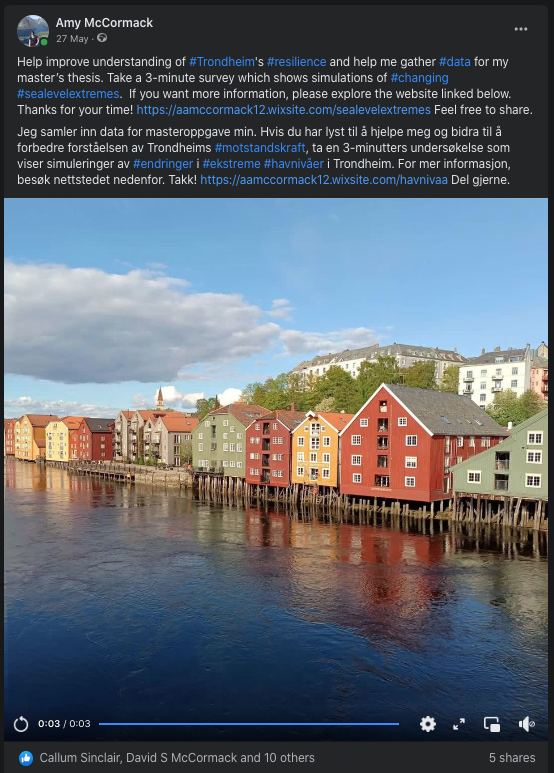
\includegraphics[width=0.7\textwidth]{fig_appendix/so_me.png}
    \caption{Social Media Post Used to Reach Subjects}{A short video playing a loop of the simulated water level extremes in Nidelva was utilised to optimise algorithms which prioritise video.}
    \label{fig:my_label}
\end{figure}


\begin{figure}[H]
    \centering
    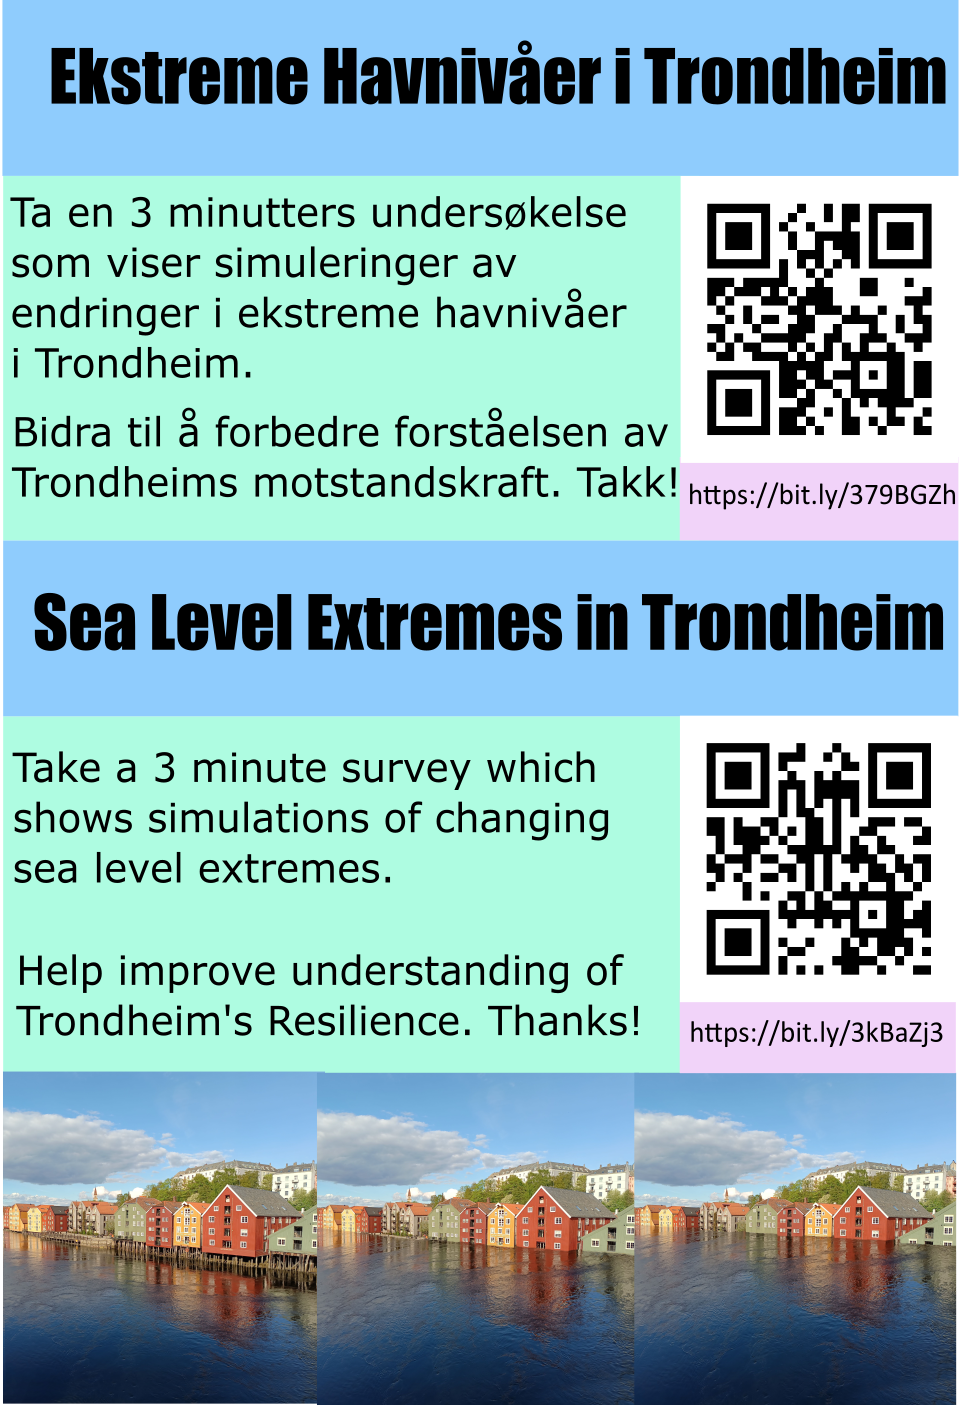
\includegraphics[width=0.9\textwidth]{fig_appendix/poster-larger.png}
    \caption{This is the poster used to reach subjects}
    \label{fig:poster}
\end{figure}

\subsection{Example Emails}
\textbf{In English}

Hi [NAME],
\paragraph{}
I am researching extreme sea level changes in Trondheim, and the population's knowledge about it. If you want to help me and possibly help improve the understanding of Trondheim's resilience, feel free to take a 3-minute survey that shows simulations of changes in extreme sea levels in Trondheim, and share it with your colleagues. 
\paragraph{}
For more information and the survey, visit the website below. Thanks! \url{https://aamccormack12.wixsite.com/havnivaa} (Norwegian) \url{https://aamccormack12.wixsite.com/sealevelextremes} (English)
\paragraph{}
If you have any questions about the research or other things, feel free to get in touch.
\paragraph{}
With best regards
\newline
Amy Anne McCormack
\paragraph{}
amymc@stud.ntnu.no
\paragraph{}

\textbf{In Norwegian}

Hei [NAVN],
\paragraph{}
Jeg forsker på ekstrem havnivåendringer i Trondheim, og befolkningens vitenskap om det.  Jeg er spesielt interessert i svar fra folk som jobber innom marine roller.
\paragraph{}
Hvis du har lyst til å hjelpe meg og bidra til å forbedre forståelsen av Trondheims motstandskraft, kan du gjerne ta en 3-minutters undersøkelse som viser simuleringer av endringer i ekstreme havnivåer i Trondheim, og dele det med dine kolleger.
\paragraph{}
For mer informasjon og undersøkelsen, besøk nettstedet nedenfor. Takk! \url{https://aamccormack12.wixsite.com/havnivaa}
\paragraph{}
Hvis du har noen spørsmål om forskningen eller masteroppgaven minn, ta gjerne kontakt.
\paragraph{}
 

Med vennlig hilsen 
\newline
Amy Anne McCormack
\paragraph{}
amymc@stud.ntnu.no



\chapter{Survey layout and Questions}


These were the questions and answer options as used in Nettskjema survey. This was accessed via a specially created website, which had full details about the research and the ability to contact the researcher. 
https://aamccormack12.wixsite.com/sealevelextremes 

The survey was designed for access via smartphones, computers and tablets. The UI was checked on each of these machines and the first targeted recipients course mates and then test engineers, so that any issues could quickly be discovered and fixed. 

\section{Example Survey - English - Grillstad}

Do you consent to these answers being used for an MSc research project?
\begin{itemize}
	\item Yes
    \item No
\end{itemize}

\newpage

\paragraph{}
How long have you known this area?
\begin{itemize}
	\item > 30 years.
    \item > 20 years
    \item > 10 years
    \item > 5 years
    \item > 1 year
    \item < 1 year
\end{itemize}

\paragraph{}
What communities in this area are you part of?
\begin{itemize}
    \item marine worker
    \item non-marine worker
    \item resident
    \item student
    \item leisure user - land
    \item leisure user - water
    \item commuter
    \item other 
\end{itemize}
Other (Write in here)
\paragraph{}

This research investigates knowledge about extreme sea levels in Trondheim, focusing on storm surges. A storm surge occurs when the weather temporarily causes water to be forced up and onto the coast.

A 20-year storm surge refers to the probability of an event, meaning there is a 1 in 20 chance (5%) of this level of event every year. This expectation changes over time, for example due to climate change.

What is your level of interest in sea level extremes?
\begin{itemize}
    \item professional interest
    \item high
    \item medium
    \item low
    \item low
    \item not interested
\end{itemize}
\paragraph{}

The following questions display simulated water levels extremes in Trondheim. The numbers in these images refer to the height above NN2000 which can be considered an approximation of mean sea level.
\paragraph{}
\includegraphics[width=1\textwidth]{fig_appendix/grillstad 2090 q.png}

Which image shows the current 20-year storm surge?
\begin{itemize}
    \item 1.2 m
    \item 2.2 m
    \item 2.7 m
    \item 3.0 m
\end{itemize}
\paragraph{}

\includegraphics[width=1\textwidth]{fig_appendix/grillstad 2090 q.png}
Which image shows the 20-year storm surge projected for 2090?
\begin{itemize}
    \item 1.2 m
    \item 2.2 m
    \item 2.7 m
    \item 3.0 m
\end{itemize}
\paragraph{}

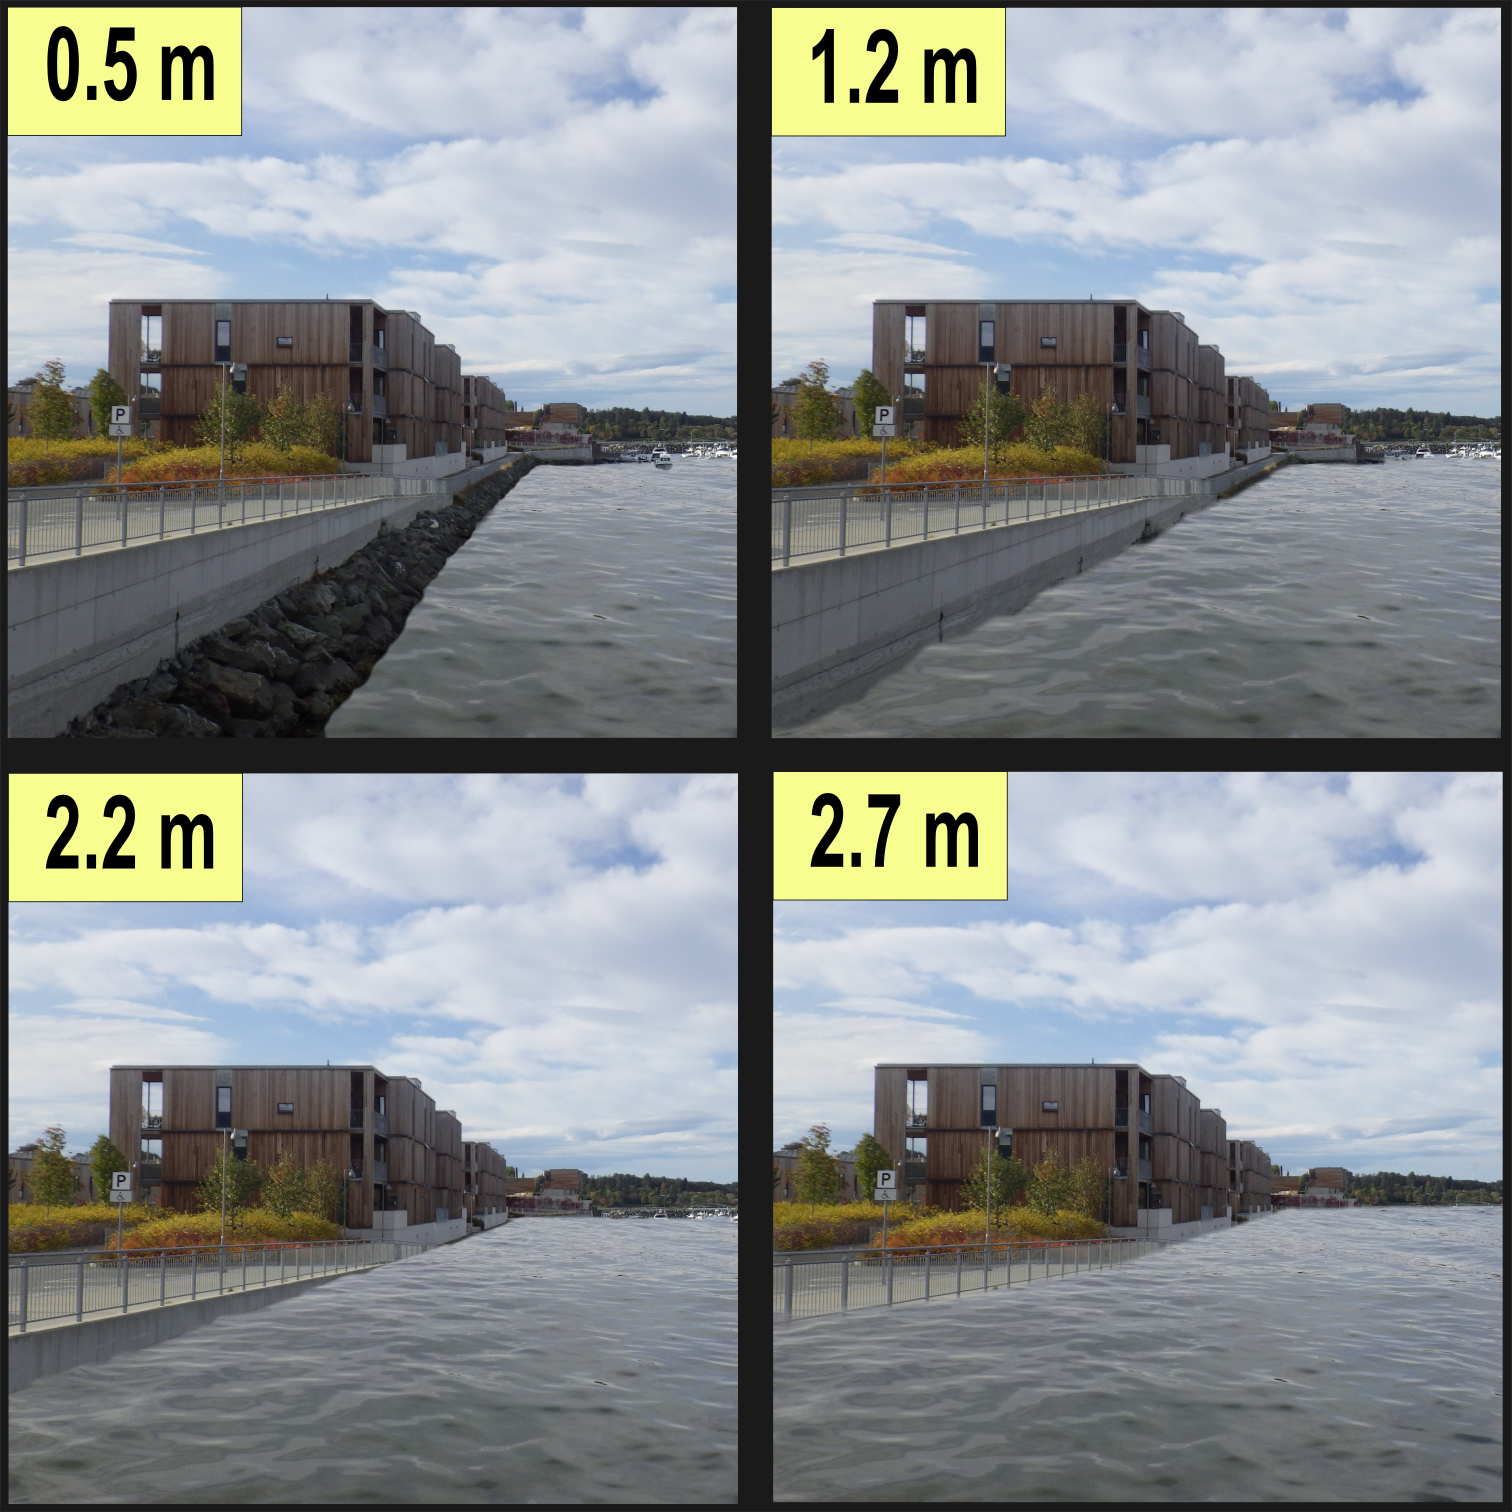
\includegraphics[width=1\textwidth]{fig_appendix/grillstad 2022 q.png}
Which image displays the current high tide?
\begin{itemize}
    \item 0.5 m
    \item 1.2 m
    \item 2.2 m
    \item 2.7 m
   \end{itemize}
\paragraph{}

Where do you get information about changes to this place?
e.g. subsidence, incidents, roadworks
\begin{itemize}
    \item personal observation
    \item family
    \item friends
    \item newspapers
    \item tv
    \item social media
    \item organisation membership
    \item municipality
\end{itemize}
\paragraph{}

Where do you get information about climate change?
\begin{itemize}
    \item personal observation
    \item family
    \item friends
    \item newspapers
    \item tv
    \item social media
    \item organisation membership
    \item peer-reviewed articles
    \item formal education
\end{itemize}

\paragraph{}
Are you concerned about climate change?
1 - not at all, 5 - very concerned
Rating Scale

\paragraph{}
How would flooding associated with sea level extremes in this area affect you?
\begin{itemize}
    \item no impact
    \item mild impact
    \item medium impact
    \item significant impact
\end{itemize}
If you would like to give more details on this, please write below.
\paragraph{}

How much do you think the sea level has changed here in the past 30 years?
\begin{itemize}
    \item + 50 cm
    \item + 20 cm
    \item + 10 cm
    \item no change
    \item - 10 cm
    \item - 20 cm 
    \item - 50 cm 
\end{itemize}
\paragraph{}

How much do you think the sea level will change in the next 30 years?
\begin{itemize}
    \item + 50 cm
    \item + 20 cm
    \item + 10 cm
    \item no change
    \item - 10 cm
    \item - 20 cm 
    \item - 50 cm 
\end{itemize}
\paragraph{}

Please tick if you remember any of these dates when coastal sea levels in Trondheim were over 2m.
\begin{itemize}
    \item 2020 February
    \item 2011 November
    \item 1999 November
    \item 1998 February
    \item 1997 February
    \item 1993 January
    \item 1990 February
    \item 1971 November
    \item I do not remember any of these events
\end{itemize}
\paragraph{}

From the following what are the major risks to people in this area?
\begin{itemize}
    \item shoreline instability
    \item storm surges
    \item waves
    \item strong winds
    \item strong tides
    \item drowning
    \item cold water shock
    \item I don't know
    \item I perceive no major risks
    \item human error
\end{itemize}
\paragraph{}

From the following what are the major risks to infrastructure in this area?
\begin{itemize}
    \item shoreline instability
    \item storm surges
    \item waves
    \item strong winds
    \item strong tides
    \item I don't know
    \item I perceive no major risks
    \item weathering
    \item precipitation
    \item human error
\end{itemize}

\paragraph{}
If you would like to give other examples of risk in this area, please write here.
\paragraph{}

How did you access this survey?
\begin{itemize}
    \item poster
    \item email
    \item social media
    \item via organisation membership
    \item via place of employment
    \item personal connection to researcher
\end{itemize}
\paragraph{}

If you would like further information on this research, please provide your e-mail address.
\newpage

\section{Example Survey - Norwegian - Brattøra }
Samtykker du at disse svarene brukes til masterforskning?
\begin{itemize}
    \item ja
    \item nei
\end{itemize}
\paragraph{}

Hvor lenge har du kjent dette området?
\begin{itemize}
	\item > 30 years.
    \item > 20 years
    \item > 10 years
    \item > 5 years
    \item > 1 year
    \item < 1 year
\end{itemize}
\paragraph{}

Hvilke samfunn i dette området er du en del av?
\begin{itemize}
    \item marinearbeider
    \item ikke-marin arbeider
    \item beboer
    \item student
    \item fritidsbruket - land
    \item fritidsbruket - vann
    \item pendler
    \item andre
\end{itemize}   

\paragraph{}
Denne forskningen undersøker kunnskap om ekstreme havnivåer i Trondheim, med fokus på stormflo. En stormflo oppstår når været midlertidig fører til at vann presses opp og inn på kysten. 
En 20-årig stormflo refererer til sannsynligheten for en hendelse. Det betyr at det er en sjanse på 1 av 20 (5 prosent) for dette nivået av begivenhet hvert år. Denne forventningen endres over tid, for eksempel på grunn av klimaendringer.
\paragraph{}

Hvor stor interesse har du for ekstreme havnivåer?
\begin{itemize}
    \item faglig interesse
    \item høy
    \item middels
    \item lav
    \item ikke interessert
\end{itemize}
\paragraph{}

Følgende spørsmål viser simulerte havnivå ekstremes i Trondheim. Tallene på disse bildene viser til høyden over NN2000 som kan betraktes som en tilnærming av gjennomsnittlig havnivå.

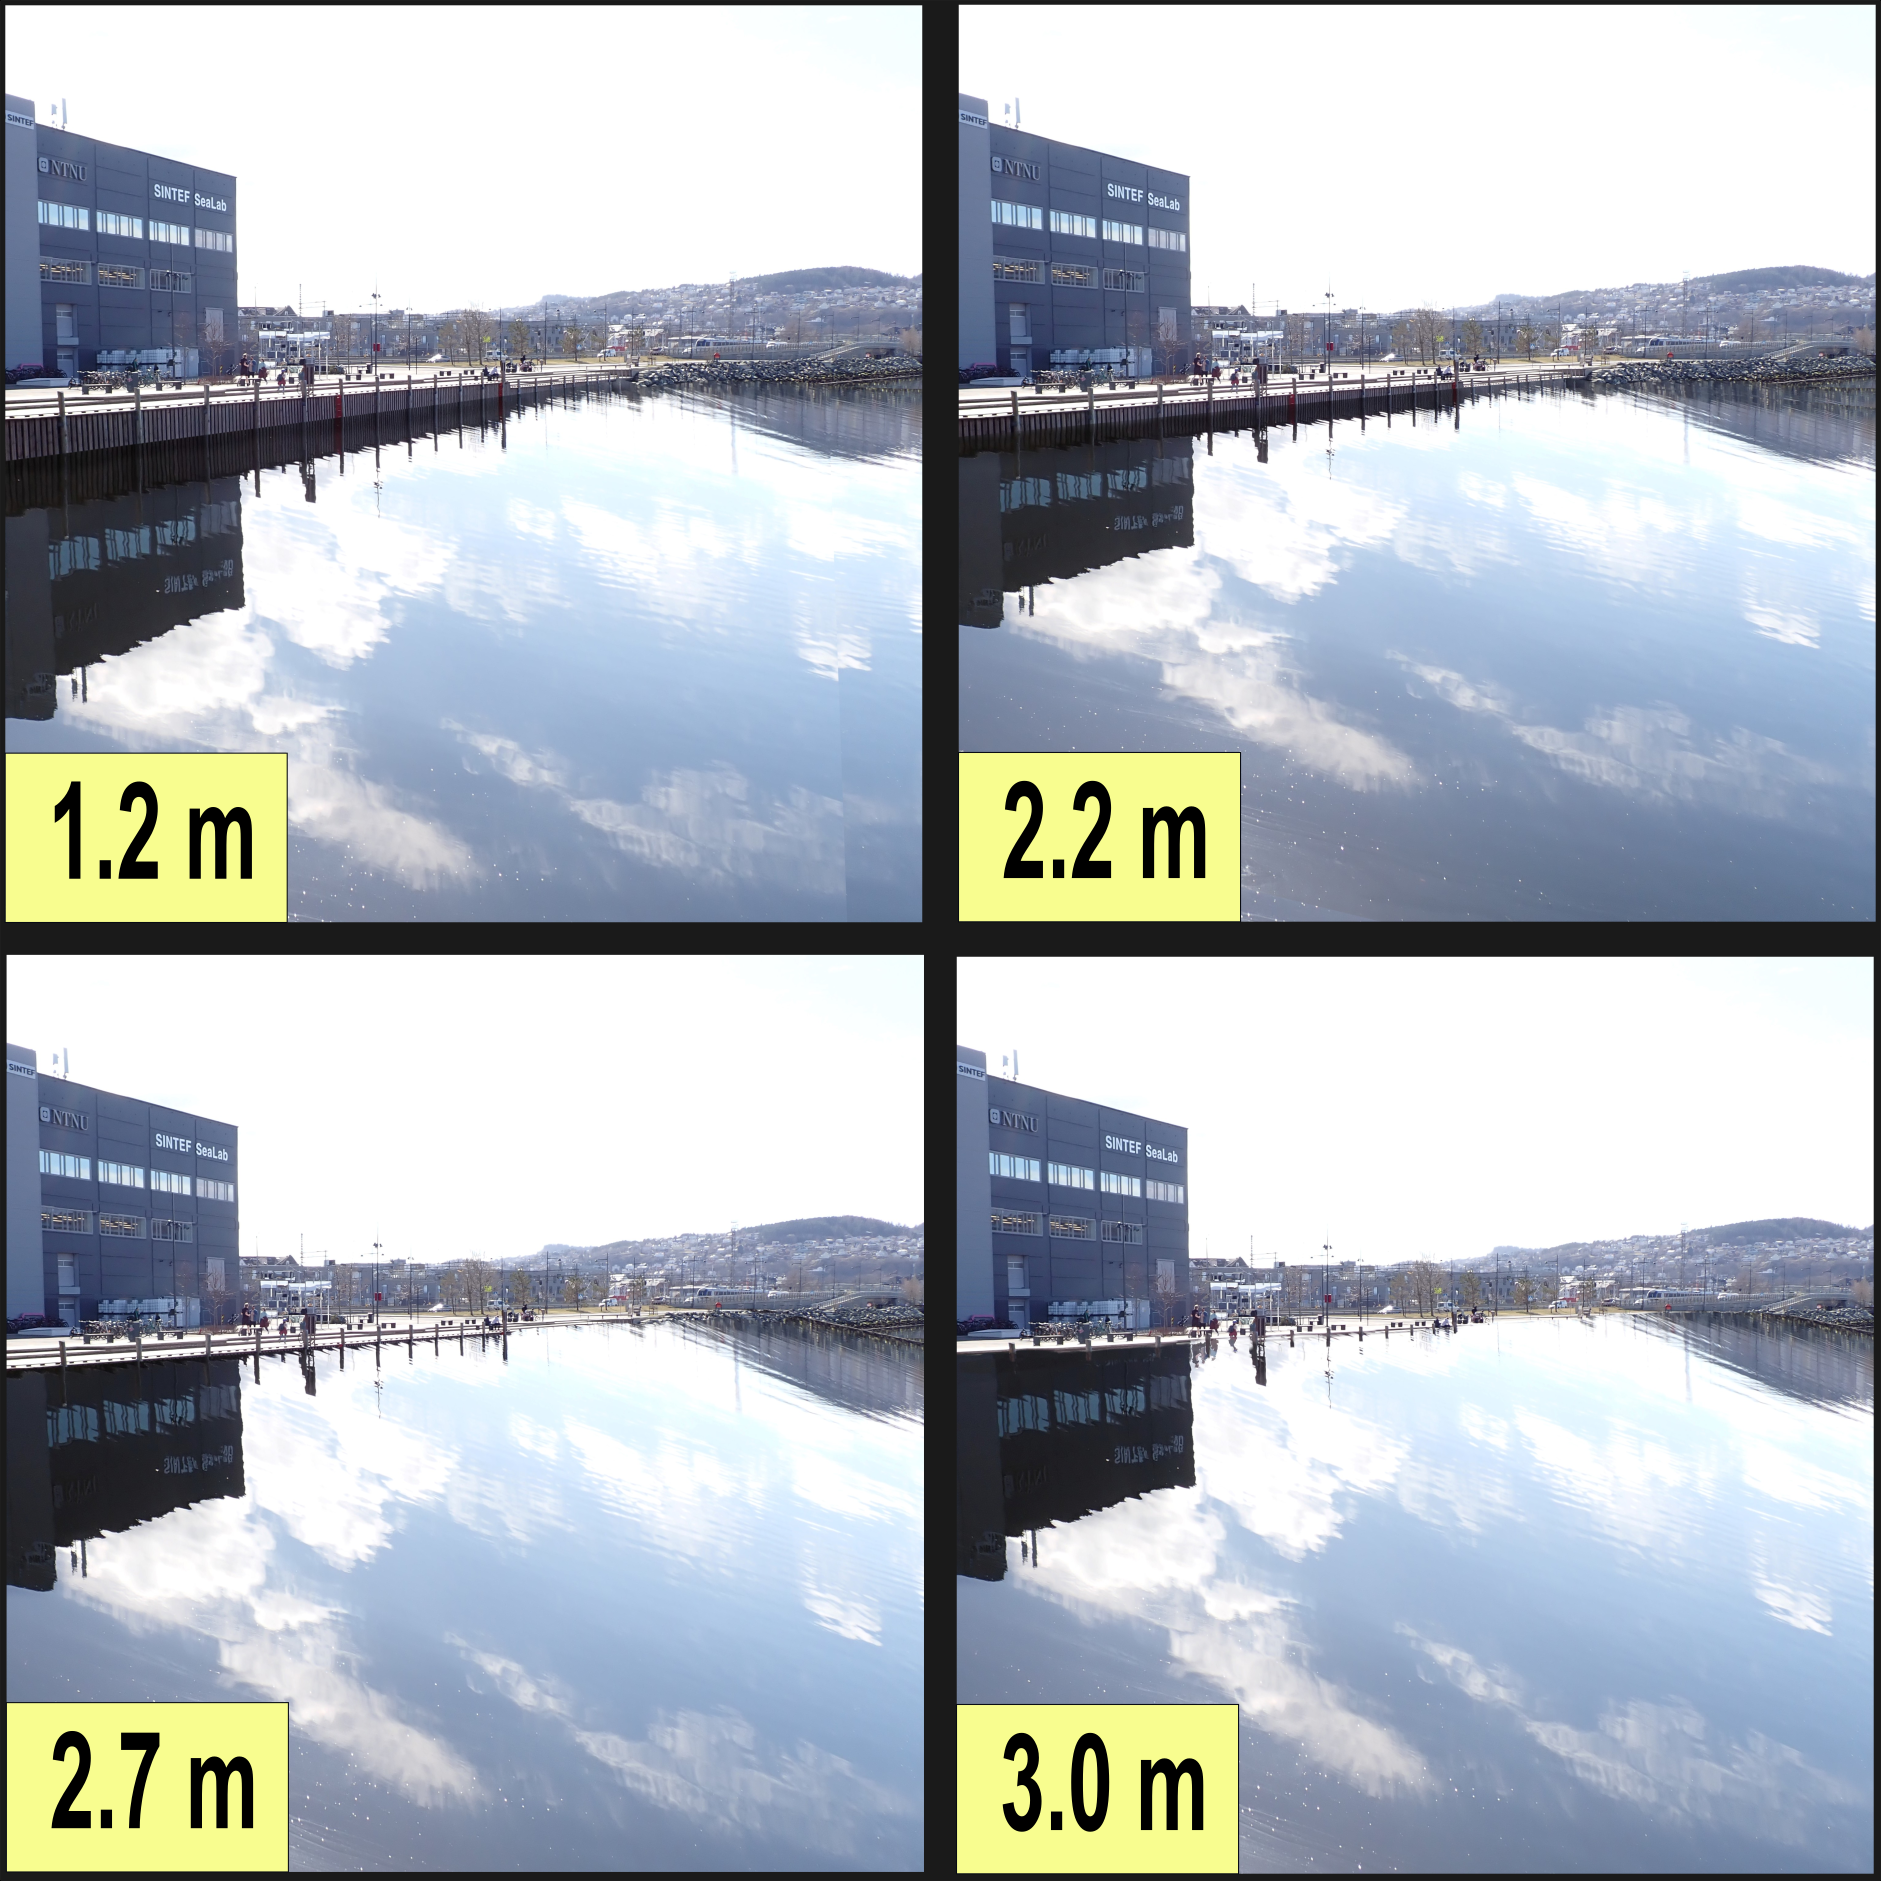
\includegraphics[width=1\textwidth]{fig_appendix/brattora 2090 q.png}
\paragraph{}
Hvilket bilde viser den nåværende 20-årene stormfloen?
\begin{itemize}
    \item 1.2 m
    \item 2.2 m
    \item 2.7 m
    \item 3.0 m
\end{itemize}
\paragraph{}

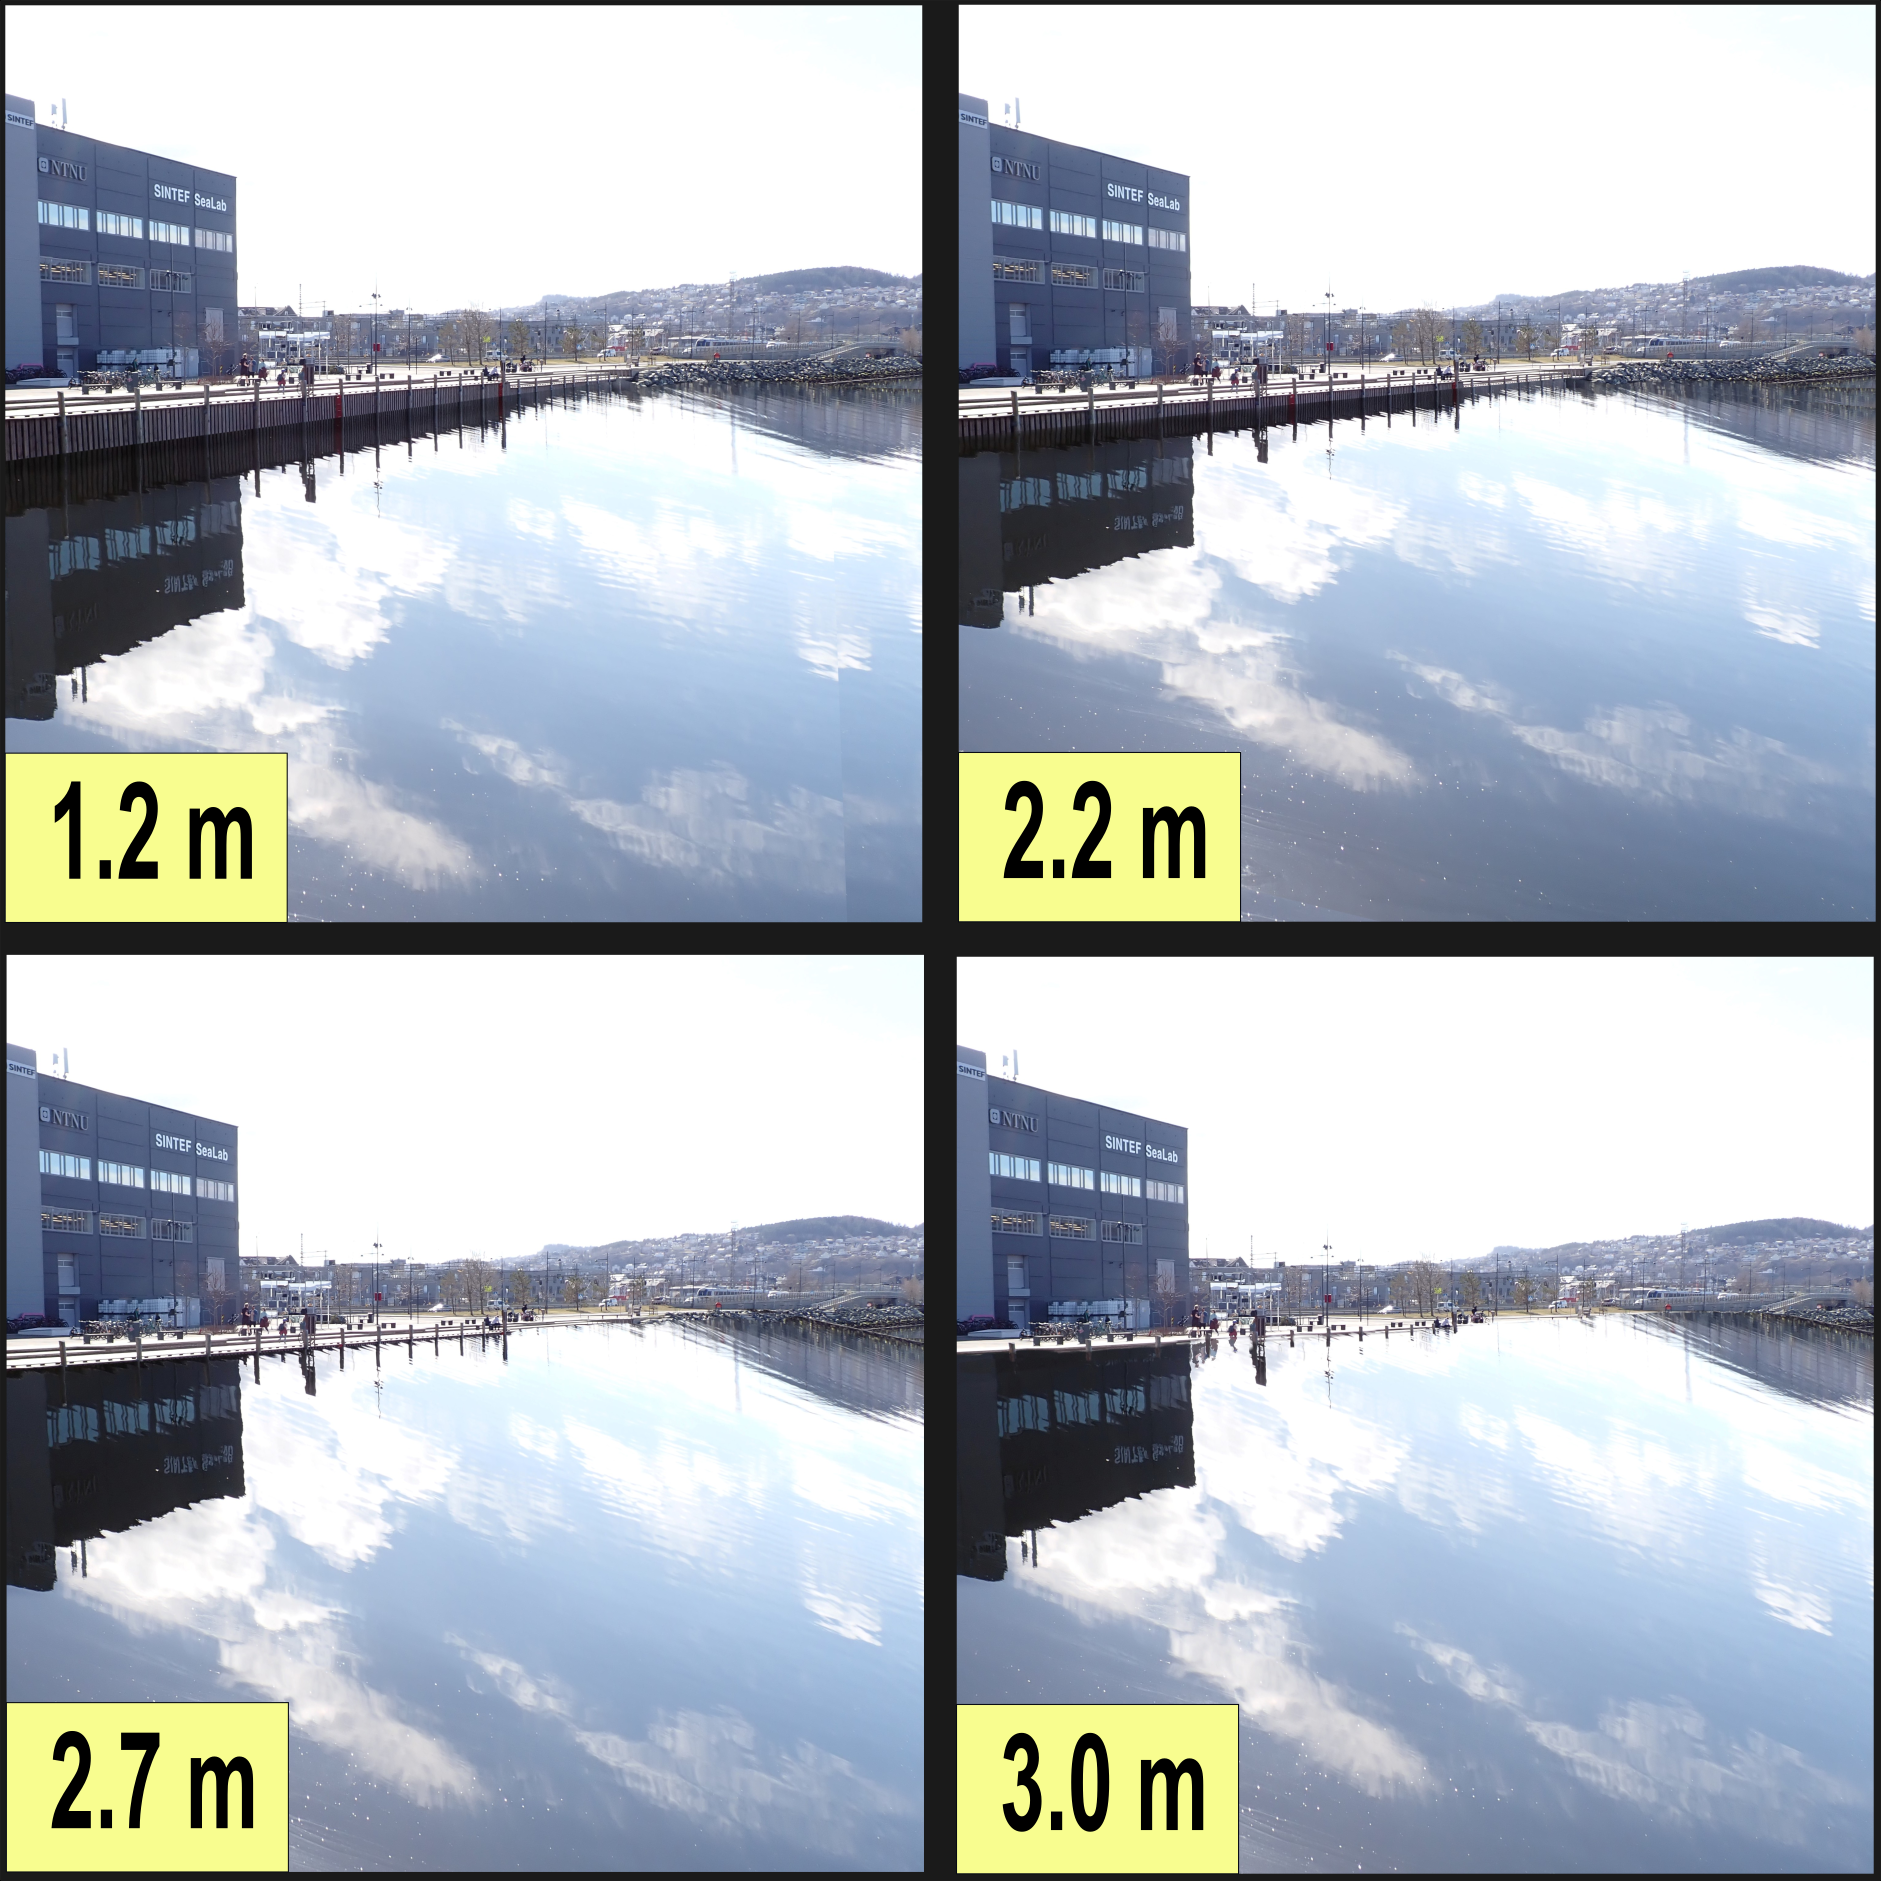
\includegraphics[width=1\textwidth]{fig_appendix/brattora 2090 q.png}
\paragraph{}
Hvilket bilde viser stedets 20-årene stormflo i 2090?
\begin{itemize}
    \item 1.2 m
    \item 2.2 m
    \item 2.7 m
    \item 3.0 m
\end{itemize}
\paragraph{}

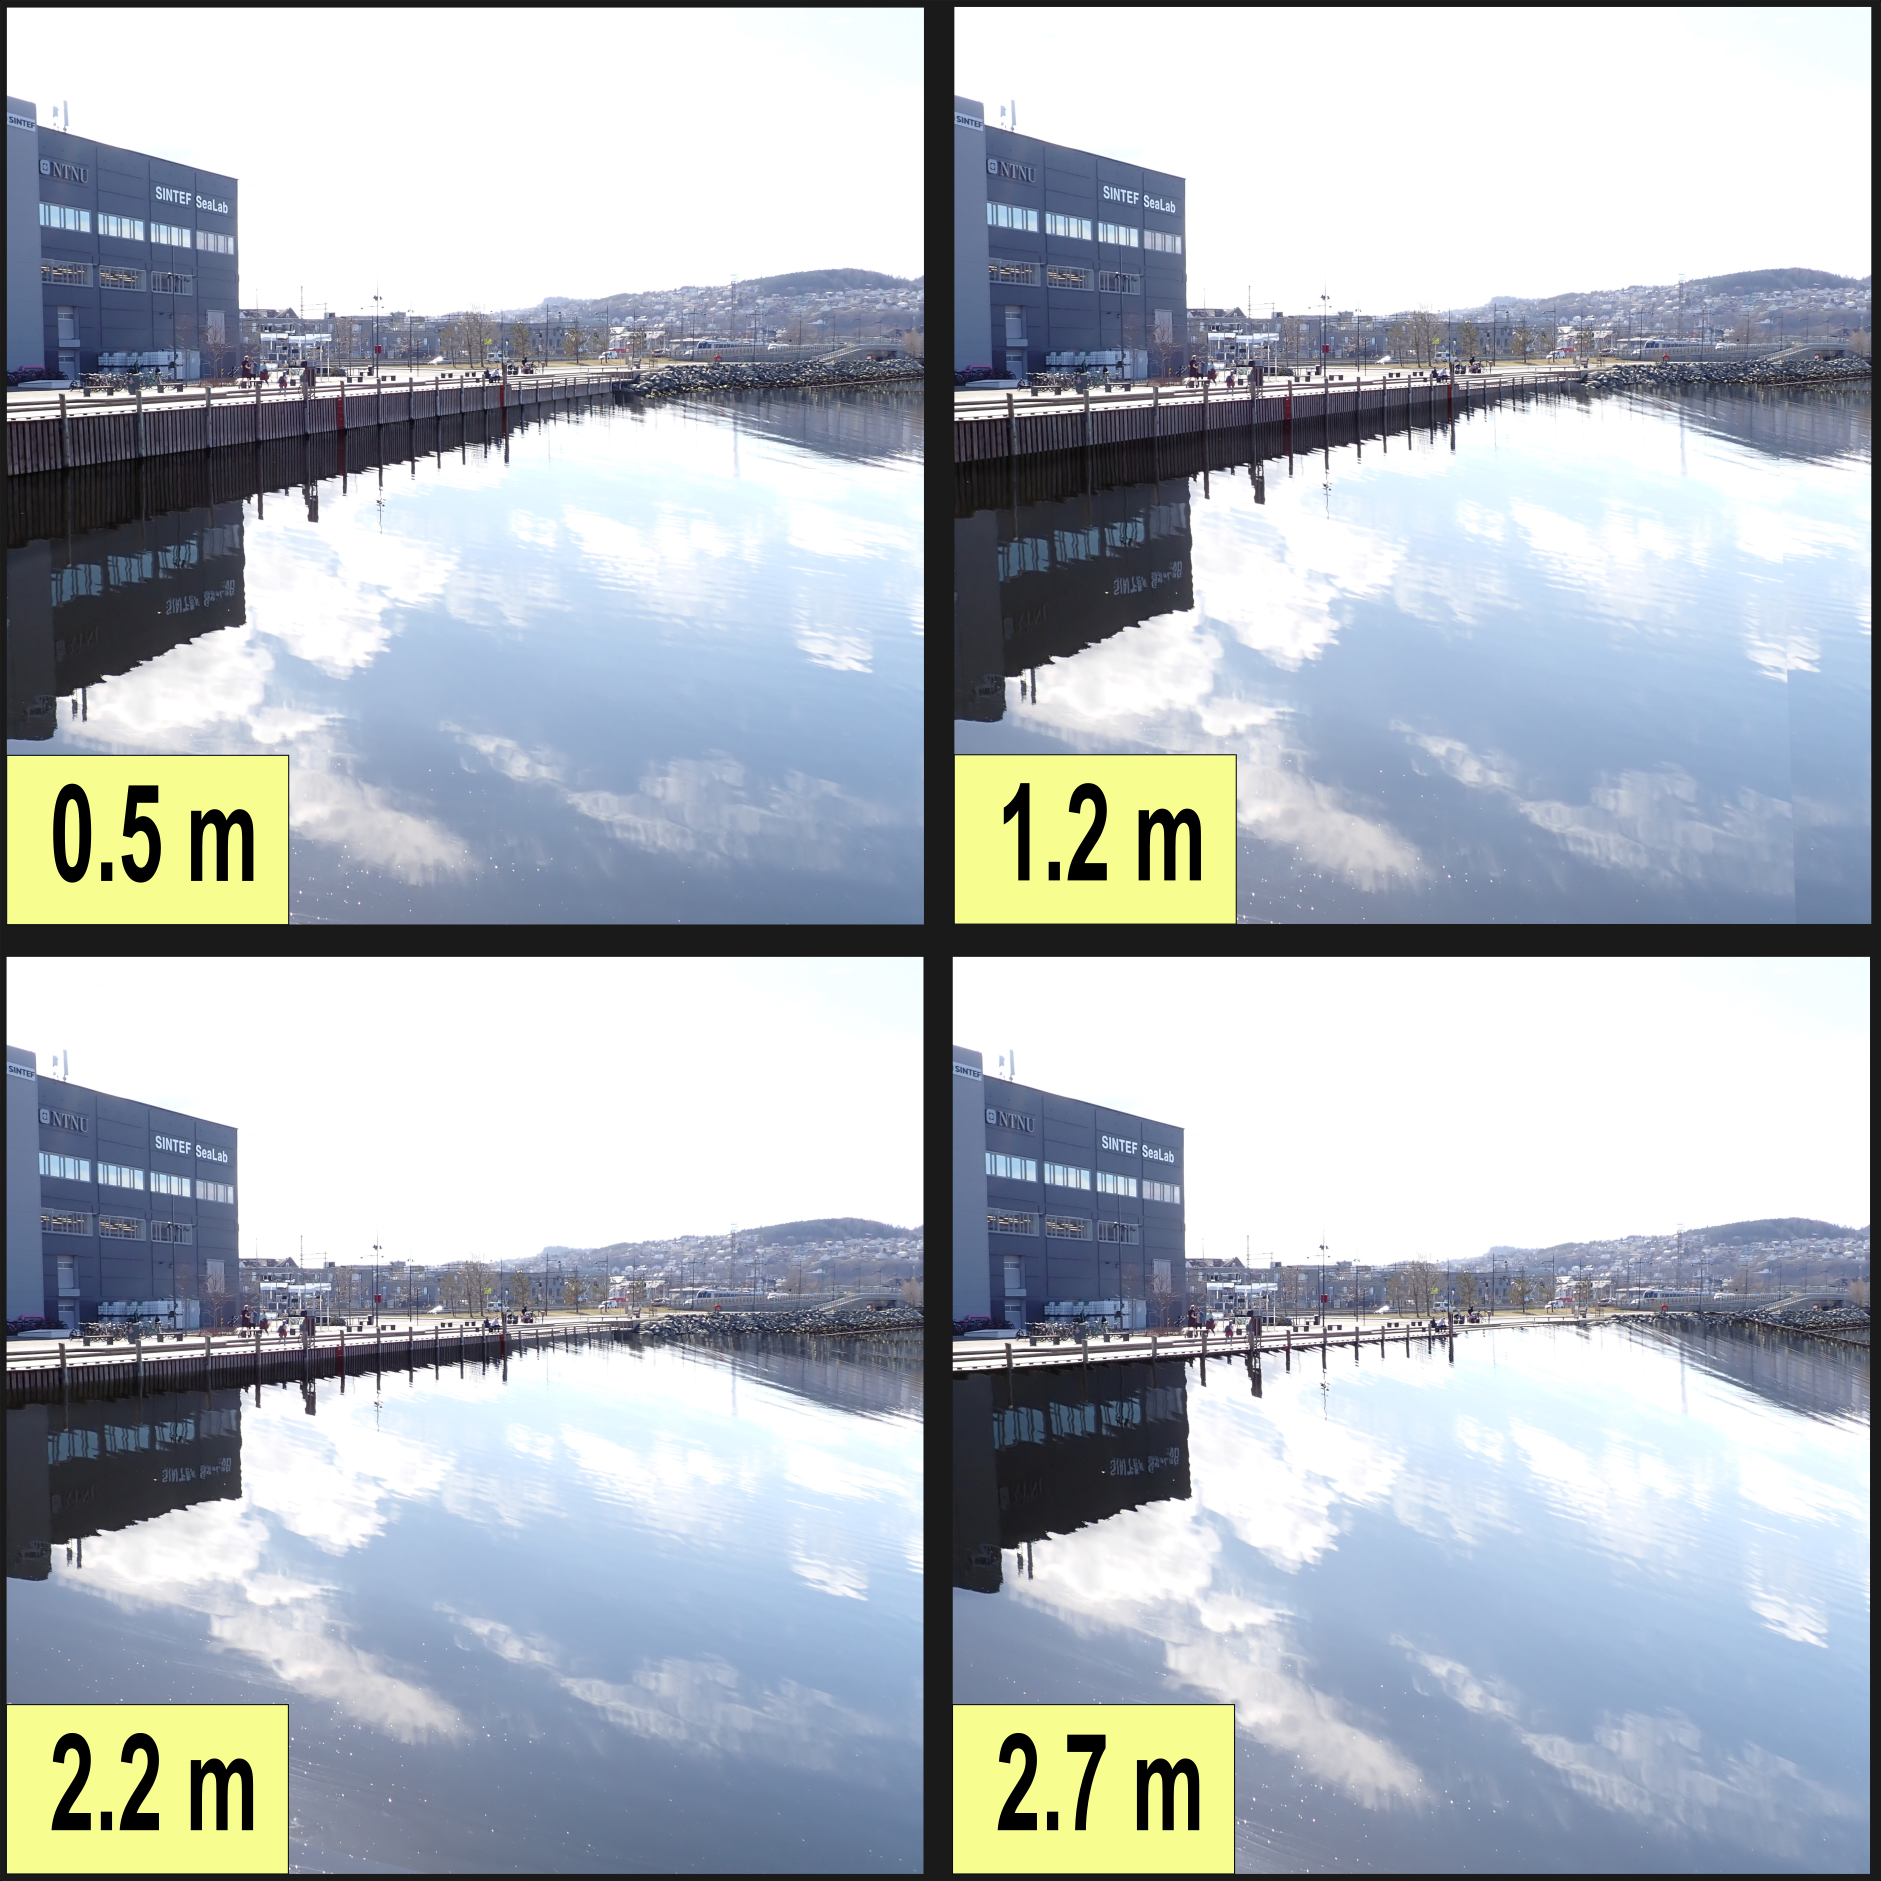
\includegraphics[width=1\textwidth]{fig_appendix/brattora 2022 q.png}
\paragraph{}
Hvilket bilde viser dette stedets høyvann i dag?
\begin{itemize}
    \item 0.5 m
    \item 1.2 m
    \item 2.2 m
    \item 2.7 m
\end{itemize}
\paragraph{}

Hvor får du informasjon om endringer på dette stedet?
f.eks. innsynkning, hendelser, veiarbeid
\begin{itemize}
    \item personlig observasjon
    \item familie
    \item venner
    \item aviser
    \item tv
    \item sosiale medier
    \item organisasjonsmedlem
\end{itemize}
\paragraph{}

Hvor får du informasjon om klimaendringer?
\begin{itemize}
    \item personlig observasjon
    \item familie
    \item venner
    \item aviser
    \item tv
    \item sosiale medier
    \item organisasjonsmedlem
    \item fagfellevurdert artikkel
    \item utdanning
\end{itemize}
\paragraph{}

Er du bekymret for klimaendringer?
1 - ikke i det hele tatt, 5 - veldig bekymret
Likertskala
\paragraph{}

Hvordan vil flom forbundet med ekstreme havnivåer i dette området påvirke deg?
\begin{itemize}
    \item ingen innvirkning
   \item mild innvirkning
   \item middels innvirkning
   \item høy innvirkning
\end{itemize}
\paragraph{}
Hvis du ønsker å gi flere detaljer om dette, vennligst skriv nedenfor
\paragraph{}

Hvor mye tror du havnivået har endret seg her de siste 30 årene?
(cm)
\begin{itemize}
    \item + 50 cm
    \item + 20 cm
    \item + 10 cm
    \item no change
    \item - 10 cm
    \item - 20 cm 
    \item - 50 cm 
\end{itemize}
\paragraph{}

Hvor mye tror du havnivået vil endre seg de neste 30 årene?
(cm)
\begin{itemize}
    \item + 50 cm
    \item + 20 cm
    \item + 10 cm
    \item no change
    \item - 10 cm
    \item - 20 cm 
    \item - 50 cm 
\end{itemize}
\paragraph{}

Kryss av hvis du husker disse ekstreme havnivå hendelsene.
Dette er alle datoene er havnivået i Trondheim har vært over 2 meter siden 1950.
\begin{itemize}
    \item 2020 februar
    \item 2011 november
    \item 1999 november
    \item 1998 februar
    \item 1997 februar
    \item 1993 januar
    \item 1990 februar
    \item 1971 november
\end{itemize}
\paragraph{}

Hva er de største risikoene for mennesker i dette området?
\begin{itemize}
    \item strandlinje ustabilitet
    \item stormflo
    \item bølger
    \item sterke vinder
    \item sterkt tidevann
    \item drukning
    \item kaldt vann sjokk
    \item Jeg vet ikke
    \item Jeg ser ingen store risikoer
    \item menneskelig feil
\end{itemize}
\paragraph{}

Hva er de største risikoene for infrastrukturen i dette området?
\begin{itemize}
    \item strandlinje ustabilitet
    \item stormflo
    \item bølger
    \item sterke vinder
    \item sterkt tidevann
    \item Jeg vet ikke
    \item Jeg ser ingen store risikoer
    \item forvitring
    \item nedbør
    \item menneskelig feil
\end{itemize}
\paragraph{}

Hvis du vil gi andre eksempler på risiko på dette området, vennligst skriv her.
\paragraph{}

Hvordan fikk du tilgang til denne undersøkelsen?
\begin{itemize}
    \item plakat
    \item e-post
    \item sosiale medier
    \item organisasjonsmedlem
    \item arbeidssted
    \item personlig tilknytning til forsker
\end{itemize}
\paragraph{}

Hvis du ønsker mer informasjon om denne forskningen, vennligst oppgi e-postadressen din.
% Include more appendices as required.

\end{document}
